% !TeX program = xelatex
\documentclass[10pt,letterpaper]{article}

% ── fonts & encoding (XeLaTeX) ────────────────────────────────────────────────
\usepackage{fontspec}
\usepackage{unicode-math}          % replaces amssymb + amsmath; XeLaTeX only
\setmainfont{TeX Gyre Pagella}
\setmathfont{TeX Gyre Pagella Math}
\setmonofont[Scale=0.88]{DejaVu Sans Mono}

% ── page layout ───────────────────────────────────────────────────────────────
\usepackage[top=1in,bottom=1in,left=0.75in,right=0.75in]{geometry}
\setlength{\columnsep}{0.25in}
\usepackage{microtype}
\setlength{\parskip}{0.3em}
\setlength{\parindent}{0pt}

\widowpenalty=10000
\clubpenalty=10000
\usepackage{needspace}

% ── tables ────────────────────────────────────────────────────────────────────
\usepackage{booktabs}
\usepackage{longtable}
\usepackage{array}
\usepackage{multirow}
\usepackage{float}
\usepackage{caption}
\captionsetup{font=small}
\usepackage{makecell}
\usepackage[section]{placeins}
\usepackage{tikz}
\usetikzlibrary{calc}
\usepackage{pgfplots}
\pgfplotsset{compat=1.18}
\usepgfplotslibrary{groupplots}

% ── §3.3 F_out word-overlap illustration ─────────────────────────────────────
\definecolor{wov@c}{RGB}{42,130,80}    % shared (green)
\definecolor{wrf@c}{RGB}{170,100,20}   % ref-only (amber)
\definecolor{wpr@c}{RGB}{50,88,150}    % pred-only (blue)
\tikzset{wbox/.style={rounded corners=2pt,inner xsep=5pt,inner ysep=2pt,
                      font=\footnotesize\ttfamily}}
\newcommand{\wov}[1]{\tikz[baseline=(n.base)]%
  \node[wbox,draw=wov@c,fill=wov@c!12,text=wov@c](n){\strut #1};}
\newcommand{\wrf}[1]{\tikz[baseline=(n.base)]%
  \node[wbox,draw=wrf@c,fill=wrf@c!12,text=wrf@c](n){\strut #1};}
\newcommand{\wpr}[1]{\tikz[baseline=(n.base)]%
  \node[wbox,draw=wpr@c,fill=wpr@c!10,text=wpr@c](n){\strut #1};}
\newcommand{\wst}[1]{\tikz[baseline=(n.base)]%
  \node[wbox,draw=black!22,fill=black!5,text=black!35](n){\strut #1};}

% ── §6.2 output-length figure series colours ─────────────────────────────────
\definecolor{cSnap}{RGB}{42,120,214}    % SnapKV    – blue
\definecolor{cPyr}{RGB}{235,104,52}     % PyramidKV – orange
\definecolor{cRandom}{RGB}{153,102,204} % Random    – purple
\definecolor{cStream}{RGB}{27,175,122}  % Streaming – teal
\definecolor{cNaive}{RGB}{237,161,0}    % Naive     – gold

% ── links & metadata ──────────────────────────────────────────────────────────
\usepackage[hyphens]{url}
\usepackage[unicode,
            colorlinks=true,
            linkcolor=black,
            citecolor=black,
            urlcolor=blue]{hyperref}

% bullet-list spacing helper (pandoc requirement)
\providecommand{\tightlist}{%
  \setlength{\itemsep}{0pt}\setlength{\parskip}{0pt}}

% section numbering: keep manual numbers already in heading text
\setcounter{secnumdepth}{-\maxdimen}

% ── metadata ──────────────────────────────────────────────────────────────────
\title{Faithfulness over Accuracy:\\Rethinking KV Cache Compression}
\author{David Bennett (dave@mytorch.net)}
\date{2026}

\begin{document}
\maketitle

\begin{abstract}
\normalsize
KV cache compression is motivated by a simple observation: long-context
inference is expensive, and many tokens in the prompt are not equally
important for generating a good response. A large body of work has
therefore focused on identifying which tokens matter --- using
accumulated attention weights {[}Zhang et al., 2023{]}, pooled key-query
alignment {[}Li et al., 2024{]}, value norms {[}Feng et al., 2025b{]},
or combinations thereof --- and evicting the rest before or during
generation.

Current compression methods are substantially less faithful to the
full-context model than standard benchmarks suggest --- and they fail
most on long-form generation, precisely where compression provides its
greatest benefit through reduced decode time. Existing papers report
near-zero accuracy degradation at 35\% retention on LongBench, a
result we reproduce. But benchmark accuracy measures task performance,
not whether the compressed model produces the same output the full model
would have produced; those are not the same thing.

We introduce two faithfulness metrics --- \emph{WTV Faithfulness}, which
measures token-distribution divergence at every generation step, and
\emph{Output Faithfulness}, which measures text-level similarity between
full and compressed model outputs --- and use them to quantify the scale
of faithfulness loss and identify the structural mechanisms responsible.

At 35\% retention, even the best selection methods diverge from the full
model on more than 30\% of words while their ground-truth scores remain
within one point of uncompressed performance. On long-form tasks, where
TPT savings compound and compression is most valuable, output similarity
differences between methods collapse beyond 100 words: intelligent
selection provides no long-form advantage over truncation or random
eviction by this measure. On short-answer tasks, post-prefill enrichment inflates output faithfulness
scores: the full-context prefill produces high-quality compressed key-value
pairs that generate correct short answers; this advantage fades as generated
tokens accumulate and dilute the enrichment effect.

WTV faithfulness reveals the structural mechanisms behind the loss.
Scattered-selection methods interact favorably with post-prefill value
enrichment; StreamingLLM's contiguous recency window contaminates value
representations with expectations about evicted context that the model
cannot satisfy at decode time.
Neither metric is sufficient on its own.

\end{abstract}

\hypertarget{introduction}{%
\section{1. Introduction}\label{introduction}}

At inference time, a transformer decoder maintains a key-value cache
that grows linearly with sequence length. For a model with \emph{L}
layers, \emph{H} heads, head dimension \emph{d}, and sequence length
\emph{T}, the KV cache occupies \emph{\(2LHdT\)} values. At long
contexts (32K--128K tokens), this cache dominates GPU memory and limits
batch size. The attention calculation itself, which uses the cache,
consumes the lion's share of the token generation time. KV cache
compression reduces these costs by retaining only a subset of the cache
entries.

Existing methods differ primarily in how they score tokens. H2O {[}Zhang
et al., 2023{]} accumulates attention scores during prefill to identify
``heavy hitter'' tokens. SnapKV {[}Li et al., 2024{]} pools attention
weights from the last observation window of queries over all key
positions. StreamingLLM {[}Xiao et al., 2023{]} retains a fixed set of
attention sink tokens plus a recency window, with no importance scoring.
H2O and SnapKV share the same broad mechanism: they process the full
prompt, compute importance scores, then evict a subset of the tokens
from the KV cache, attending only to the retained subset during
generation.

We make the following contributions:

\begin{itemize}
\item
  \textbf{Ground-truth evaluation as the wrong criterion}: Standard
  benchmarks measure whether a compressed model gives the correct
  answer, not whether it behaves the same way as the full model. We
  argue this is the wrong objective for compression and analyze several
  distinct failure modes of GT evaluation as a compression metric
  (§3.1).
\item
  \textbf{WTV faithfulness metric (\(F_{\text{WTV}}\))}: Entropy-weighted
  total variation between the full and compressed model's next-token
  distributions, computed on a shared generation prefix. Suppresses isolated
  catastrophic divergences to focus on steps where distributional agreement
  actually matters (§3.2).
\item
  \textbf{Output faithfulness metric (\(F_{\text{out}}\))}: Word-level
  F1 between the full model's generated output and the compressed
  model's generated output, with no external ground-truth reference.
  Reveals two complementary effects: post-prefill enrichment inflates
  short-answer \(F_{\text{out}}\) for selection methods by producing
  high-quality compressed key-value pairs (§6.1), masking faithfulness
  differences on the tasks where compression is cheapest; and a consistent
  ranking across methods that corroborates the WTV ordering (§3.4, §4.4).
\item
  \textbf{Eviction geometry determines faithfulness}:
  Scattered-selection methods (SnapKV, PyramidKV) achieve high WTV
  faithfulness because their distributed retention geometry interacts
  favorably with post-prefill value enrichment. Block eviction methods
  (StreamingLLM) are substantially less faithful.
  A controlled gap-geometry experiment confirms the geometry
  mechanism (§5.2--§5.3).
\end{itemize}

\hypertarget{background-and-related-work}{%
\section{2. Background and Related
Work}\label{background-and-related-work}}

\textbf{KV cache eviction.} Scissorhands {[}Liu et al., 2023{]}
introduced the \emph{persistence of importance} hypothesis: tokens that
accumulate high attention during prefill remain important throughout
generation, so the attention-score history is a reliable eviction
criterion. H2O {[}Zhang et al., 2023{]} operationalizes this by
maintaining a running sum of per-head attention scores and evicting the
lowest-scoring tokens. SnapKV {[}Li et al., 2024{]} refines the scoring
by pooling attention weights from only the last \emph{w} queries (an
observation window), better reflecting the queries that will matter at
decode time, using post-RoPE (Rotary Position Embedding {[}Su et al., 2024{]}) vectors. StreamingLLM {[}Xiao et al.,
2023{]} abandons score computation entirely, retaining a fixed set of
attention sink tokens plus a sliding recency window. In its original
online design the cache is bounded continuously throughout processing
--- the model never builds a full-length KV cache --- which bounds time
to first token (TTFT) at the cost of discarding all non-recent
non-sink content.

\textbf{Value-norm scoring.} VATP {[}EMNLP 2024{]} scores tokens by the
product of attention weight and L1 value norm, observing that attention
sinks receive high attention but near-zero V-norm. Feng et
al.~{[}2025b{]} provide a theoretical justification via an upper bound
on output perturbation, recommending a two-stage selector combining
attention weights with projected value norms \(\|V \cdot W^O\|_1\). We
test a simpler additive combination of KQ alignment and raw V-norm and
find it does not improve over KQ alignment alone.

\textbf{Layer- and head-adaptive budgets.} Ada-KV {[}NeurIPS 2025{]},
HeadKV {[}ICLR 2025{]}, and DuoAttention {[}ICLR 2025{]} allocate
different token budgets to different attention heads within each layer.
PyramidKV {[}Cai et al., 2024{]} takes a complementary approach,
allocating different total budgets to different transformer layers ---
more KV slots at lower layers (which the original authors find need
broader context) and fewer at higher layers (where task-relevant
patterns have already concentrated). Both families operate on top of an
existing token-scoring method and can in principle be combined with any
of the per-token importance metrics discussed above. Our method uses a
uniform budget per layer, and we note that the structural corruption
problem (§5) applies to any of these methods that rely on the KV
patching mechanism regardless of how budgets are distributed.

\textbf{Query-aware and dynamic selection.} Quest {[}Tang et al., ICML
2024{]} departs from static prefill-time selection by performing
per-decode-step KV retrieval. At each generation step, the current query
is used to retrieve the most relevant KV blocks from the full cache,
limiting attention to the top-K pages. This eliminates the assumption
that token importance is fixed at prefill time and instead adapts the
attended set to each query. The tradeoff is computational: Quest
requires a custom CUDA kernel for block-sparse attention, making
integration into existing inference stacks non-trivial. Our structural
corruption analysis applies to Quest only partially --- because Quest
retrieves complete contiguous blocks rather than individual scattered
tokens, gaps within each attended block are minimal, though inter-block
gaps remain.


\textbf{Token merging.} CaM {[}Y. Zhang et al., 2024{]} and its
successor KVMerger {[}Wang et al., 2024{]} take a different approach:
rather than evicting low-importance tokens, they \emph{merge} pairs of
similar KV vectors, collapsing them into a single weighted average and
reducing cache size without introducing empty positions. This avoids the
causal gap problem entirely --- the retained set is contiguous --- but
produces keys and values that are off-manifold linear combinations not
present in any normal prompt. The faithfulness cost of such merging
versus structural corruption from eviction is an open question. CaM does
not support grouped-query attention (GQA {[}Ainslie et al., 2023{]}), limiting its applicability to
GQA models such as Llama-3.1.

\textbf{Evaluation critique.} Chen et al.~{[}2025{]} (``Pitfalls of KV
Cache Compression'') provide empirical evidence that standard KV
compression benchmarks are insufficient for evaluating compression
quality and that compression methods perform significantly worse than
their published numbers suggest under stricter evaluation conditions.
This finding aligns with and provides additional evidence for our
faithfulness-based critique of the field.

\textbf{Faithfulness evaluation.} To our knowledge, no prior KV cache
compression work has systematically evaluated faithfulness to
full-context outputs as a primary metric. The closest work is in model
distillation and generation evaluation, where output-to-output
comparison is common {[}Papineni et al., 2002; Zhang et al., 2020{]}. We
adapt perplexity-based and embedding-based comparison to the compression
setting.

\textbf{KVPress framework.} Devoto et al.~{[}2025{]} introduce KVPress,
a unified framework for KV cache compression research. Our method can be
implemented as a KVPress press subclass, providing compatibility with
the associated leaderboard and ecosystem.

\hypertarget{faithfulness-metrics}{%
\section{3. Faithfulness Metrics}\label{faithfulness-metrics}}

\hypertarget{why-ground-truth-evaluation-falls-short}{%
\subsection{3.1 Why Ground-Truth Evaluation Falls
Short}\label{why-ground-truth-evaluation-falls-short}}

The papers that introduced SnapKV, PyramidKV, and StreamingLLM evaluated
their methods by running the compressed model on benchmark tasks and
scoring its outputs against human-labeled reference answers
{[}Li et al., 2024; Cai et al., 2024; Xiao et al., 2023{]}.
Practitioners are now deploying these methods based on those results.

The implicit assumption underlying this evaluation --- and the
deployment decisions that follow from it --- is that a method which
scores well on the benchmark is a good approximation of the full model.
This assumption fails for a simple reason: the metric never actually
compares the compressed model's outputs to the full model's outputs.
Two methods can score identically while producing completely different
text, and the metric will never notice. Ground-truth evaluation has
four distinct failure modes as a compression metric.
\Needspace{4\baselineskip}
\begin{itemize}
\item
  \textbf{The scoring functions do not reliably measure correctness.}
  Of the 16 tasks, only three (TREC, PassageCount, PassageRetrieval)
  score a prediction as binary right or wrong. The remaining thirteen
  tasks use word-overlap F1 or ROUGE-L, which give partial credit for
  surface overlap with a reference and are unreliable even for that
  purpose. F1 is order-blind: a prediction that reverses who won and
  who lost a game scores 1.0 because it reuses the same words
  (Figure~\ref{fig:fout-f1}, panel b). ROUGE-L penalizes valid
  syntactic reorderings. Both are blind to paraphrase: a semantically
  perfect answer in different words scores zero (panel d).

\begin{figure}[H]
\noindent\begin{minipage}{\linewidth}
\small
\renewcommand{\arraystretch}{1.7}
% legend
\begin{tabular}{@{}l@{\enspace}l@{\quad}l@{\enspace}l@{\quad}l@{\enspace}l@{\quad}l@{\enspace}l@{}}
  \wov{word} & shared &
  \wrf{word} & reference only &
  \wpr{word} & prediction only &
  \wst{the}  & stripped (article)
\end{tabular}

\smallskip\noindent\rule{\linewidth}{0.3pt}\smallskip

\textbf{(a)}\ \textit{Standard case --- partial word overlap}

\begin{tabular}{@{}p{1.9cm}@{\hskip 0.3em}l@{}}
  Reference  & \wov{Napoleon}\ \wov{was}\ \wrf{exiled}\ \wov{to}\ \wov{Elba}\ \wov{in}\ \wov{1814} \\
  Prediction & \wov{Napoleon}\ \wov{was}\ \wpr{sent}\ \wov{to}\ \wov{Elba}\ \wov{in}\ \wov{1814}
\end{tabular}\par\noindent
\makebox[\linewidth][r]{\footnotesize\textcolor{black!50}{%
  F1:\enspace$|$shared$|=6$\enspace P$=6/7$\enspace R$=6/7$}\enspace
  \textcolor{wov@c}{\textbf{F1$\,=0.857$}}}

\noindent\makebox[\linewidth][r]{\footnotesize\textcolor{black!50}{%
  ROUGE-L:\enspace LCS$=6$\enspace P$=6/7$\enspace R$=6/7$}\enspace
  \textcolor{wov@c}{\textbf{ROUGE-L$\,=0.857$}}}

\smallskip\noindent\rule{\linewidth}{0.3pt}\smallskip

\textbf{(b)}\ \textit{Failure --- identical words, opposite meaning}

\begin{tabular}{@{}p{1.9cm}@{\hskip 0.3em}l@{}}
  Reference  & \wov{Team}\ \wov{A}\ \wov{defeated}\ \wov{Team}\ \wov{B}\ \wov{in}\ \wov{overtime} \\
  Prediction & \wov{Team}\ \wov{B}\ \wov{defeated}\ \wov{Team}\ \wov{A}\ \wov{in}\ \wov{overtime}
\end{tabular}\par\noindent
\makebox[\linewidth][r]{\footnotesize\textcolor{black!50}{%
  F1:\enspace$|$shared$|=7$\enspace P$=7/7$\enspace R$=7/7$\enspace(order-blind --- winner/loser swapped)}\enspace
  \textcolor{wrf@c}{\textbf{F1$\,=1.000$}}}

\noindent\makebox[\linewidth][r]{\footnotesize\textcolor{black!50}{%
  ROUGE-L:\enspace LCS$=5$\enspace P$=5/7$\enspace R$=5/7$\enspace(order-sensitive via LCS, still high)}\enspace
  \textcolor{wrf@c}{\textbf{ROUGE-L$\,=0.714$}}}

\smallskip\noindent\rule{\linewidth}{0.3pt}\smallskip

\textbf{(c)}\ \textit{Robust case --- reordered words, identical content}

\begin{tabular}{@{}p{1.9cm}@{\hskip 0.3em}l@{}}
  Reference  & \wst{The}\ \wov{prime}\ \wov{minister}\ \wov{resigned}\ \wov{yesterday} \\
  Prediction & \wov{Yesterday}\ \wst{the}\ \wov{prime}\ \wov{minister}\ \wov{resigned}
\end{tabular}\par\noindent
\makebox[\linewidth][r]{\footnotesize\textcolor{black!50}{%
  F1:\enspace$|$shared$|=4$\enspace P$=4/4$\enspace R$=4/4$\enspace(order-blind --- handles reordering correctly)}\enspace
  \textcolor{wov@c}{\textbf{F1$\,=1.000$}}}

\noindent\makebox[\linewidth][r]{\footnotesize\textcolor{black!50}{%
  ROUGE-L:\enspace LCS$=3$\enspace P$=3/4$\enspace R$=3/4$\enspace(\emph{yesterday} falls outside the LCS)}\enspace
  \textcolor{wrf@c}{\textbf{ROUGE-L$\,=0.750$}}}

\smallskip\noindent\rule{\linewidth}{0.3pt}\smallskip

\textbf{(d)}\ \textit{Failure --- synonymous outputs, zero score}

\begin{tabular}{@{}p{1.9cm}@{\hskip 0.3em}l@{}}
  Reference  & \wst{The}\ \wrf{patient}\ \wrf{recovered}\ \wrf{completely}\ \wrf{after}\ \wrf{treatment} \\
  Prediction & \wst{The}\ \wpr{sick}\ \wpr{person}\ \wpr{got}\ \wpr{better}\ \wpr{following}\ \wpr{therapy}
\end{tabular}\par\noindent
\makebox[\linewidth][r]{\footnotesize\textcolor{black!50}{%
  F1:\enspace$|$shared$|=0$\enspace P$=0/6$\enspace R$=0/5$\enspace(paraphrase blindness)}\enspace
  \textcolor{wrf@c}{\textbf{F1$\,=0.000$}}}

\noindent\makebox[\linewidth][r]{\footnotesize\textcolor{black!50}{%
  ROUGE-L:\enspace LCS$=0$\enspace P$=0/6$\enspace R$=0/5$\enspace(paraphrase blindness)}\enspace
  \textcolor{wrf@c}{\textbf{ROUGE-L$\,=0.000$}}}

\smallskip\noindent\rule{\linewidth}{0.3pt}
\end{minipage}
\caption{Surface-overlap metric failure modes (word-level F1 and ROUGE-L).}
\label{fig:fout-f1}
\end{figure}

\item
  \textbf{A single reference does not cover all correct answers.}
  For QA and summarization tasks, the reference is one human-written
  answer or summary. A model that answers correctly but differently ---
  ``midnight'' instead of ``12\,AM'', ``sent to'' instead of ``exiled
  to'' --- receives no credit. ``Ground-truth accuracy'' ends up
  measuring surface similarity to one person's phrasing rather than
  whether the answer is right.

\item
  \textbf{Faithful errors are penalized.}

  If the full-context model
  produces a wrong answer, a compressed model that faithfully reproduces
  that same wrong answer scores 0 on ground truth. The metric penalizes
  faithfulness when it produces the wrong answer for the ``right
  reasons.'' A compression method should not be penalized for being a
  good approximation.

\item
  \textbf{Low full-model accuracy amplifies these problems.}

  The base models used here (Llama-3.1-8B and Mistral-7B-v0.3) achieve
  macro-average GT scores of approximately 25 out of 100 on LongBench.
  Our own evaluations of the instruction-tuned variants on the same
  benchmark yield 33.2\% for Llama-3.1-8B-Instruct and 32.8\% for
  Mistral-7B-Instruct-v0.3 (Appendix~A) --- meaning roughly 67\% of what
  each instruct model generates does not overlap with the ground-truth
  reference. For that majority of output, the metric is entirely blind
  to whether compression changed the model's behavior: the compressed
  and uncompressed models could produce identical text or completely
  different text, and the GT score would be the same either way.

  The papers that introduced these methods evaluated instruction-tuned
  variants and report somewhat higher baselines --- approximately 41--43\%
  for LLaMA-3-8B-Instruct and Mistral-7B-Instruct-v0.2 in the PyramidKV
  and SnapKV evaluations {[}Cai et al., 2024; Li et al., 2024{]} --- but
  the same logic applies: when the full model fails to match the reference
  on the majority of examples, GT cannot detect compression effects for
  that majority.

\end{itemize}


\hypertarget{kl-faithfulness}{%
\subsection{3.2 WTV Faithfulness}\label{wtv-faithfulness}}

We need a metric that addresses ground-truth evaluation's failures. Rather than comparing
the outputs of the original and compressed models to a human-written reference,
we need to directly compare the compressed model to the original model to determine
whether it is faithful to the original.

Compression fidelity is best evaluated by comparing the compressed model's next-token
distributions directly to the full model's, on a shared generation sequence.
The uncompressed model generates a response \(y^*\)
= (\(y^*_1, \ldots, y^*_L\)) from the full context. Both the full model
and each compressed model are then teacher-forced on this shared token
sequence: at step \emph{t}, the full model conditions on {[}\emph{c},
\emph{q}, \(y^*_1, \ldots, y^*_{t-1}\){]} and the compressed model
conditions on {[}\emph{ĉ}, \emph{q}, \(y^*_1, \ldots, y^*_{t-1}\){]}.
The metric is entropy-weighted total variation, averaged across all generation steps
(Figure~\ref{fig:eval-setup}):

\[
F_{\text{WTV}} =
  \frac{\displaystyle\frac{1}{L}\sum_{t=1}^{L}
    H\!\left(P_{\text{full},t}\right)\cdot
    \mathrm{TV}\!\left(P_{\text{full},t},\, P_{\text{comp},t}\right)}%
  {\displaystyle\frac{1}{L}\sum_{t=1}^{L}
    H\!\left(P_{\text{full},t}\right)}
\]
where \(\mathrm{TV}(P,Q)=\tfrac{1}{2}\sum_x|P(x)-Q(x)|\) is total variation distance
and \(H(P)=-\sum_x P(x)\log P(x)\) is entropy of the full model's distribution.

\begin{figure}[H]
\centering
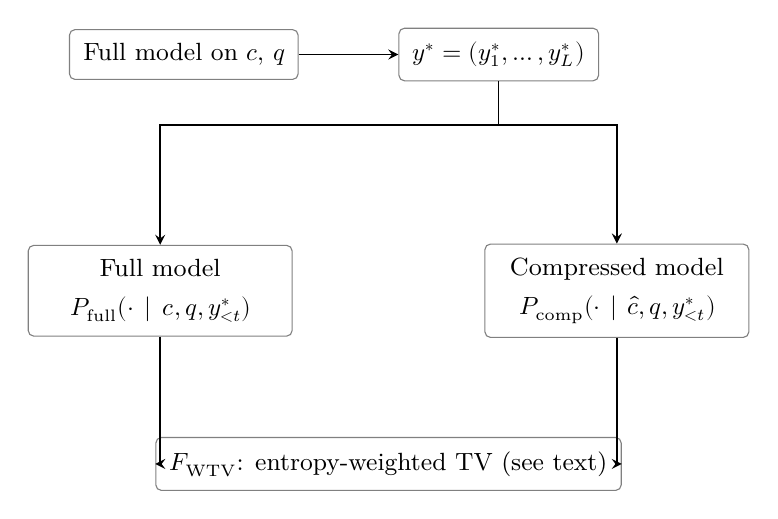
\begin{tikzpicture}[
  box/.style={draw=black!50, rounded corners=2pt, inner sep=5pt,
              text centered, font=\small},
  arr/.style={->, >=stealth, semithick}
]
  \node[box] (fm) at (1.5,0) {Full model on $c,\,q$};
  \node[box] (ys) at (5.5,0) {$y^* = (y^*_1,\ldots,y^*_L)$};
  \draw[arr] (fm) -- (ys);

  \node[box, text width=3.0cm, align=center] (pfull) at (1.2,-3.0)
    {Full model\\[3pt]$P_{\text{full}}(\cdot \mid c,q,y^*_{<t})$};
  \node[box, text width=3.0cm, align=center] (pcomp) at (7.0,-3.0)
    {Compressed model\\[3pt]$P_{\text{comp}}(\cdot \mid \hat{c},q,y^*_{<t})$};

  \coordinate (fk) at ($(ys.south)+(0,-0.55)$);
  \draw (ys.south) -- (fk);
  \draw[arr] (fk) -| (pfull.north);
  \draw[arr] (fk) -| (pcomp.north);

  \node[box] (kl) at (4.1,-5.2)
    {$F_{\text{WTV}}$: entropy-weighted TV (see text)};

  \draw[arr] (pfull.south) |- (kl.west);
  \draw[arr] (pcomp.south) |- (kl.east);
\end{tikzpicture}
\caption{$F_{\text{WTV}}$ evaluation setup. Both models are teacher-forced on the full model's
output $y^*$, anchoring every comparison to the full model's actual behavior.}
\label{fig:eval-setup}
\end{figure}

\(F_{\text{WTV}}\) ranges from 0 (identical distributions at every step) to 1
(maximally divergent at every high-entropy step). The entropy weight
\(H(P_{\text{full},t})\) in the numerator focuses the metric on steps where
distributional agreement actually matters. When the full model assigns near-certain
probability to a single token, that step contributes little to the metric regardless
of what the compressed model does --- and compressed models are unlikely to diverge
there anyway, since the dominant token is nearly forced. Steps where the full model is
genuinely uncertain --- where shifts in probability mass across the vocabulary carry
real information cost, and where compression-induced context differences are most
likely to matter --- are weighted in proportion to that uncertainty. The \([0,1]\) bound makes
absolute values interpretable across methods and budgets.

Conditioning all methods on the same shared token sequence \(y^*\) eliminates
path-dependence: a method whose compressed context causes early divergence would
otherwise be evaluated on a different downstream sequence than a more faithful
method, making scores incomparable across methods.

This metric captures distributional agreement at the token probability level, not
just which token is selected by greedy decoding: a method that shifts probability
mass from the correct token to semantically similar alternatives --- invisible to
both greedy accuracy measures and ground-truth benchmarks --- registers as a
faithfulness cost in \(F_{\text{WTV}}\).

\hypertarget{output-faithfulness}{%
\subsection{3.3 Output Faithfulness}\label{output-faithfulness}}

WTV faithfulness measures how well the compressed model's internal
distributions match the full model's. A complementary question is: how
similar is the text the compressed model actually generates?

We define \textbf{Output Faithfulness} (\(F_{\text{out}}\)) as:

\[
F_{\text{out}} = \frac{1}{N} \sum_{i=1}^{N}
  \text{f1}\!\left(\hat{y}^{\,\text{full}}_i,\, \hat{y}^{\,\text{comp}}_i\right)
\]

where f1 is word-level F1 between the full model's prediction and the
compressed model's prediction on example i. Both predictions are
generated autoregressively with greedy decoding; no external
ground-truth reference is used.

Word-level F1 is computed after lowercasing, removing articles (a, an,
the), and stripping punctuation --- the same normalization used by
LongBench for extractive QA evaluation. The metric ranges from 0 (no
word overlap) to 1 (identical output text).

\(F_{\text{out}}\) addresses the failure modes of ground-truth
evaluation directly: it does not compare to any external reference, so
faithful errors are not penalized and accidental correctness is not
rewarded. It also provides partial credit in two cases that binary
accuracy metrics miss: when both models produce the same wrong answer
(they are being equally and faithfully wrong), and when one model's
output partially overlaps the other's (approximation with some drift).
For a compression method that is a good approximation,
\(F_{\text{out}}\) should be high regardless of whether the underlying
outputs are ``correct.''


\textbf{Caveat emptor on output-text metrics.}

\nopagebreak
\(F_{\text{out}}\) is more principled than ground-truth evaluation, but word-level F1
introduces its own distortions that any output-text measurement
inherits. Panels (b) and (d) of Figure~\ref{fig:fout-f1} apply directly:
\(F_{\text{out}}\) is blind to word-order reversals and synonymous paraphrases for
the same reasons the GT metrics are, since it applies the same normalization to
model-to-model comparisons. Readers should treat \(F_{\text{out}}\) scores and any
generated output-based measurement with appropriate skepticism.


These limitations are why \(F_{\text{WTV}}\) is the primary distributional metric
rather than \(F_{\text{out}}\): \(F_{\text{WTV}}\) operates at the distribution
level at every generation step, is insensitive to output length, and requires no
string matching.


\hypertarget{why-these-two-metrics}{%
\subsection{3.4 Why These Two Metrics?}\label{why-these-two-metrics}}

Other distributional or behavioral metrics are possible ---
Jensen-Shannon divergence (bounded and symmetric), rank correlation
between full and compressed top-k token rankings (sensitive to ordering,
blind to probability mass), logit cosine similarity (no
information-theoretic meaning), or calibration error against ground
truth (reintroduces the external reference both metrics are designed to
avoid). We choose \(F_{\text{WTV}}\) and \(F_{\text{out}}\) for
complementary reasons.

\(F_{\text{WTV}}\) is the primary distributional metric because its
[0,\,1] bound makes absolute values interpretable across methods and
budgets, and the entropy weighting focuses the metric on generation
steps where distributional agreement actually matters (near-deterministic
steps are downweighted regardless). 

We use word-level F1 for
\(F_{\text{out}}\) because it requires no external reference, reuses the
scoring function LongBench already applies to extractive QA, and provides a
human-readable scale: 0 means no word overlap with the full model's
output; 100 means identical text. This keeps faithfulness evaluation on
the same footing as the ground-truth evaluation it is designed to improve on.

\(F_{\text{WTV}}\) and \(F_{\text{out}}\) are measuring different things:
\(F_{\text{WTV}}\) measures \textbf{distributional faithfulness}, which is how
similar the two models' probability distributions are over the
vocabulary at every generation step, while \(F_{\text{out}}\) measures
\textbf{behavioral faithfulness}, how similar the two models' final
generated texts are.
\(F_{\text{out}}\) provides a human-interpretable reference point; \(F_{\text{WTV}}\) is
more informative for comparing methods against each other.

KL divergence has a direct information-theoretic interpretation and
decomposes cleanly per step, making it attractive as a faithfulness
metric. Its fundamental problem is that it gives the wrong weight to the steps
that matter. At near-deterministic steps --- where the full model assigns near-certain
probability to one token --- the dominant token's contribution \(P(x)\log(P(x)/Q(x))\)
is amplified by its high probability, making KL large even when the actual choice is
nearly forced. At genuinely uncertain steps, where context is actively guiding the
response and a compression-induced shift in the distribution has real consequences,
probability mass is spread across many tokens, producing smaller individual
contributions and lower KL. The metric implicitly underweights exactly the
context-sensitive decision points where faithfulness matters most.

KL is also unbounded: whenever the compressed model assigns near-zero probability to a
token the full model places meaningful mass on, KL diverges without limit at that step,
and a single spike can dominate the per-example mean. Positional displacement from
structural corruption produces exactly these spikes, which WTV also sees --- but WTV's
total variation distance is bounded in \([0,1]\) at every step, so no spike can
dominate the mean. WTV's entropy weight \(H(P_t)\) further corrects the primary
problem by explicitly upweighting the uncertain steps that KL underweights.

The practical consequence is that KL can rank methods differently from
both WTV and \(F_{\text{out}}\): the positional-displacement spikes that
SnapKV's gap structure produces inflate KL relative to WTV, and the
ranking that WTV and \(F_{\text{out}}\) agree on is the more behaviorally
meaningful one.

\hypertarget{main-experiments}{%
\section{4. Experiments}\label{main-experiments}}

\hypertarget{setup-1}{%
\subsection{4.1 Setup}\label{setup-1}}

\textbf{kvpress}

All KV-cache eviction methods in this paper are implemented using
\texttt{kvpress} v0.5.4, a library that provides a unified hook-based
interface for post-prefill cache compression. Each method performs a
full, unrestricted prefill pass over the complete prompt, scores each
token's KV entry using post-prefill attention weights, and evicts
lower-scoring entries from the KV cache before the first decode step.

The kvpress documentation explicitly recommends combining
\texttt{KeyRerotationPress} with \texttt{StreamingLLMPress} ``to fully
match the implementation described in the paper.'' We adopt the kvpress
recommended configuration for Streaming (\texttt{StreamingLLMPress} +
\texttt{KeyRerotationPress}). For scattered-selection methods (SnapKV,
PyramidKV), re-rotation worsens WTV at every rate and budget on
both models, so those use no position adjustment after eviction.

Streaming uses kvpress's post-prefill adaptation: a full prefill is
performed before trimming (§5.1), so retained tokens' hidden states are
computed with access to the complete context. This departs from the
original StreamingLLM online design's TTFT advantage but puts Streaming
on equal footing with SnapKV and PyramidKV.

\textbf{Benchmarks}
\\LongBench v1, 16 English tasks, 100 examples per task.

\textbf{Models}
\\Base: Llama-3.1-8B and Mistral-7B-v0.3 (fp16) evaluated at 35\%, 50\% and 65\% retention budget.
\\Instruct: Llama-3.1-8B-Instruct and Mistral-7B-Instruct-v0.3 (fp16), evaluated at absolute token budgets of 256 and 1024 tokens (§§4.2--4.4).

\textbf{Hyperparameters}
\\Base model experiments use retention rates 35/50/65\% with \texttt{window\_size=128}; PyramidKV uses \texttt{beta=20}; Streaming uses \texttt{n\_sink=4}.
\\Instruct experiments use \texttt{window\_size=8} for SnapKV and PyramidKV at budget~=~256 
(PyramidKV's per-layer average would collapse to uniform distribution at the default 
\texttt{window\_size=32}); \texttt{window\_size=32} is used at budget~=~1024.
\\Full implementation details below; per-task instruct breakdowns in Appendices~A--C.

\textbf{Compression Methods Tested}
\\We benchmarked the baseline uncompressed prompt and five compression methods,
one of which compresses the input prompt while the remaining four all prune the KV
cache after prefill.

\begin{enumerate}
\item 
\textbf{Full context} - This uses the 
complete prompt with no compressions and serves as the baseline for comparison.

\item
\textbf{Naive} This method truncates the prompt
to form a shorter, self-consistent input with no modification to the KV patching or
attention mask calculations. The prompt is split into a 10\% head (literal first tokens)
and a 90\% recency tail, concatenated to form a new prompt at the budgeted length.

\item
\textbf{Streaming} - The KV Cache is pruned reserving the first 4 attention sink tokens plus a
recency window to fill the remaining budget, following StreamingLLM’s selection rule [Xiao et
al., 2023]. Retained keys are re-rotated to compact positions after eviction
(\texttt{KeyRerotationPress}), consistent with the kvpress recommended configuration.

\item
\textbf{SnapKV} - Prunes the KV cache based on the attention weights pooled over the last 128-token
observation window {[}Li et al., 2024{]}. No position adjustment after eviction.

\item
\textbf{PyramidKV} - Follows the same SnapKV-style attention scoring, but with a layer-adaptive
budget that allocates more KV slots to lower layers and fewer to higher layers [Cai et al., 2024].
The per-layer budget follows a linear decay controlled by beta=20; budgets are clamped to
\texttt{[window\_size, sequence\_length]}. No position adjustment after eviction.


\end{enumerate}


The last \texttt{window\_size} tokens (the observation window) are
always retained by being assigned high scores; we use
\texttt{window\_size=128} throughout (kvpress stock default is 64). For
GQA models such as Llama-3.1-8B (32 Q-heads, 8 KV-heads), kvpress
aggregates scores via mean-pooling across query heads sharing a KV head.

\hypertarget{gt-evaluation}{%
\subsection{4.2 Ground-Truth Results}\label{gt-evaluation}}

Ground-truth (GT) accuracy measures whether a compressed model produces outputs
that match human-written reference answers. Table~\ref{tab:gt-allrates} shows macro-averaged scores
across all rates on both models.
Per-task results at 65\% retention appear in Appendix~A.

\begin{table}[H]
\centering
\small
\captionsetup{justification=centering}
\caption{Mean ground-truth accuracy by method and retention rate (higher is better)}
\label{tab:gt-allrates}
\begin{minipage}[t]{0.49\textwidth}
\centering
\textbf{Llama-3.1-8B}\\[0.4em]
\begin{tabular}{@{}lrrrrr@{}}
\toprule
& \multicolumn{3}{c}{Base} & \multicolumn{2}{c}{Instruct}\\
\cmidrule(lr){2-4}\cmidrule(lr){5-6}
Method & 35\% & 50\% & 65\% & $b$=256 & $b$=1024\\
\midrule
Naive      & 20.8 & 21.6 & 23.4 & 16.9 & 20.1\\
Streaming  & 23.1 & 23.5 & 23.8 & 26.4 & 26.9\\
SnapKV     & \textbf{24.8} & \textbf{24.9} & 25.0 & 30.7 & 31.5\\
Pyr        & \textbf{24.8} & 24.2 & \textbf{25.1} & \textbf{31.2} & \textbf{31.6}\\
Random     & 22.7 & 23.1 & 24.2 & --- & ---\\
\midrule
Full       & 25.0 & 25.0 & 25.0 & 33.2 & 33.2\\
\bottomrule
\end{tabular}
\end{minipage}%
\hfill
\begin{minipage}[t]{0.49\textwidth}
\centering
\textbf{Mistral-7B-v0.3}\\[0.4em]
\begin{tabular}{@{}lrrrrr@{}}
\toprule
& \multicolumn{3}{c}{Base} & \multicolumn{2}{c}{Instruct}\\
\cmidrule(lr){2-4}\cmidrule(lr){5-6}
Method & 35\% & 50\% & 65\% & $b$=256 & $b$=1024\\
\midrule
Naive      & 20.2 & 21.1 & 22.0 & 16.7 & 20.9\\
Streaming  & 21.4 & 22.1 & 22.7 & 23.5 & 25.8\\
SnapKV     & \textbf{23.0} & \textbf{23.3} & \textbf{23.5} & 31.3 & \textbf{32.2}\\
Pyr        & \textbf{23.0} & 22.9 & \textbf{23.5} & \textbf{31.6} & 32.1\\
Random     & 21.8 & 22.8 & 22.9 & --- & ---\\
\midrule
Full       & 23.6 & 23.6 & 23.6 & 32.8 & 32.8\\
\bottomrule
\end{tabular}
\end{minipage}
\par\smallskip
\textbf{Bold} = best compressed method per column. Full context is the reference (rate-independent).
\end{table}


These are the numbers that support the claim that compression is nearly free.
On Llama, SnapKV and PyramidKV at 65\% retention score 25.0 and 25.1 --- matching
or exceeding the full-model baseline of 25.0. At 35\% retention they score 24.8,
within one percentage point. On Mistral the picture is identical: SnapKV and Pyr
match Full (23.6) at 65\%, and drop by at most 0.6 points at 35\%. A reader of the
papers introducing these methods would conclude from these numbers that aggressive
compression is essentially lossless.

That conclusion is an artifact of what GT measures. Because it scores against external
reference answers rather than the full model's outputs (§3.1), it cannot distinguish a
compressed model that closely replicates the full model from one that produces completely
different text that happens to contain the right answer words. With macro-average GT
scores around 25\%, two models can post identical scores while getting entirely different
examples correct --- the compressed model need not overlap at all with the full model to
match its GT score. 

Scattered-selected methods --- those that distribute token evictions across the entire prompt --- 
all cluster within 1 point across all rates.
The true cost of compression is not visible using the ground truth metric.
On instruct budgets, Naive separates from the rest because
at extreme compression, prompt truncation destroys exact-match retrieval accuracy. 

\hypertarget{kl-faithfulness-main-results}{%
\subsection{4.3 WTV Faithfulness: Main Results}\label{wtv-faithfulness-main-results}}
Table~\ref{tab:t3} shows mean WTV faithfulness. The per-task breakdown is in Appendix~B.

\begin{table}[H]
\centering
\small
\captionsetup{justification=centering}
\caption{Mean WTV faithfulness (\(F_{\text{WTV}}\)) by method, retention rate, and token budget.}
\label{tab:t3}
\begin{minipage}[t]{0.49\textwidth}
\centering
\textbf{Llama-3.1-8B}\\[0.4em]
\begin{tabular}{@{}lrrrrr@{}}
\toprule
& \multicolumn{3}{c}{Base} & \multicolumn{2}{c}{Instruct}\\
\cmidrule(lr){2-4}\cmidrule(lr){5-6}
Method & 35\% & 50\% & 65\% & $b$=256 & $b$=1024\\
\midrule
Naive      & 0.200 & 0.162 & 0.139 & 0.537 & 0.406\\
Streaming  & 0.126 & 0.105 & 0.085 & 0.281 & 0.227\\
SnapKV     & \textbf{0.065} & \textbf{0.046} & 0.030 & \textbf{0.179} & \textbf{0.096}\\
Pyr        & \textbf{0.065} & 0.064 & \textbf{0.025} & 0.180 & 0.097\\
Random     & 0.107 & 0.082 & 0.061 & --- & ---\\
\bottomrule
\end{tabular}
\end{minipage}%
\hfill
\begin{minipage}[t]{0.49\textwidth}
\centering
\textbf{Mistral-7B-v0.3}\\[0.4em]
\begin{tabular}{@{}lrrrrr@{}}
\toprule
& \multicolumn{3}{c}{Base} & \multicolumn{2}{c}{Instruct}\\
\cmidrule(lr){2-4}\cmidrule(lr){5-6}
Method & 35\% & 50\% & 65\% & $b$=256 & $b$=1024\\
\midrule
Naive      & 0.161 & 0.132 & 0.116 & 0.602 & 0.467\\
Streaming  & 0.174 & 0.153 & 0.132 & 0.363 & 0.307\\
SnapKV     & \textbf{0.065} & \textbf{0.044} & \textbf{0.027} & \textbf{0.251} & \textbf{0.153}\\
Pyr        & \textbf{0.065} & 0.074 & 0.028 & 0.259 & 0.159\\
Random     & 0.156 & 0.120 & 0.088 & --- & ---\\
\bottomrule
\end{tabular}
\end{minipage}
\par\smallskip
Lower is better. \textbf{Bold} = best value per column.
Base = retention rate; Instruct = absolute token budget.
\end{table}

The finding here is more striking.
The scattered-selection methods (SnapKV, PyramidKV) are substantially more faithful than
block eviction (Streaming), truncation (Naive), and random eviction
at every rate. Among scattered-selection methods, SnapKV leads at most base-model
configurations, with PyramidKV marginally better at 65\%.
At instruct budgets, SnapKV continues to lead; Streaming
narrows substantially relative to Naive as budget tightens, suggesting
block eviction degrades more gracefully than truncation at extreme
compression.


\hypertarget{output-faithfulness-results}{%
\subsection{4.4 Output Faithfulness
Results}\label{output-faithfulness-results}}

Table~\ref{tab:t4} shows the output faithfulness results (per-task breakdown in Appendix~C).  
Here we can get a clearer picture of the true cost of compression.

\begin{table}[H]
\centering
\small
\captionsetup{justification=centering}
\caption{Mean \(F_{\text{out}}\) by method, retention rate, and token budget (per-task breakdown in Appendix C)}
\label{tab:t4}
\begin{minipage}[t]{0.49\textwidth}
\centering
\textbf{Llama-3.1-8B}\\[0.4em]
\begin{tabular}{@{}lrrrrr@{}}
\toprule
& \multicolumn{3}{c}{Base} & \multicolumn{2}{c}{Instruct}\\
\cmidrule(lr){2-4}\cmidrule(lr){5-6}
Method & 35\% & 50\% & 65\% & $b$=256 & $b$=1024\\
\midrule
Naive      & 46.9 & 52.1 & 68.6 & 24.9 & 37.0\\
Streaming  & 51.8 & 56.4 & 61.1 & 56.1 & 62.0\\
SnapKV     & 66.8 & \textbf{73.2} & 78.5 & \textbf{72.0} & \textbf{81.9}\\
Pyr        & \textbf{66.9} & 64.2 & \textbf{79.0} & 71.1 & 81.8\\
Random     & 49.9 & 55.3 & 61.1 & 58.0 & 67.7\\
\bottomrule
\end{tabular}
\end{minipage}%
\hfill
\begin{minipage}[t]{0.49\textwidth}
\centering
\textbf{Mistral-7B-v0.3}\\[0.4em]
\begin{tabular}{@{}lrrrrr@{}}
\toprule
& \multicolumn{3}{c}{Base} & \multicolumn{2}{c}{Instruct}\\
\cmidrule(lr){2-4}\cmidrule(lr){5-6}
Method & 35\% & 50\% & 65\% & $b$=256 & $b$=1024\\
\midrule
Naive      & 52.6 & 56.9 & 60.0 & 25.7 & 33.9\\
Streaming  & 53.8 & 57.4 & 61.0 & 47.1 & 54.3\\
SnapKV     & 74.0 & \textbf{79.0} & \textbf{83.7} & \textbf{63.9} & \textbf{76.1}\\
Pyr        & \textbf{74.1} & 68.8 & 83.5 & 63.0 & 74.9\\
Random     & 52.0 & 57.1 & 64.0 & 48.2 & 57.9\\
\bottomrule
\end{tabular}
\end{minipage}
\par\smallskip
Higher is better. \textbf{Bold} = best per column. Base = retention rate; Instruct = absolute token budget.
\end{table}

At 35\% retention on Llama --- the setting where GT showed essentially no degradation ---
the best selection methods (SnapKV, PyramidKV) produce outputs that share only 67\% of
words with what the full model would have said. At 65\% the gap is 21 points; at 50\%,
27 points. The compression tax that GT evaluation was hiding is between 20 and 33
percentage points depending on rate. On Mistral the picture is qualitatively the same:
25 points at 35\%, 16 at 65\%.

The instruct model at budget~=~256 looks better at first glance (SnapKV: Llama 72\%,
Mistral 64\%). This is partly misleading for the same structural reason as GT: a
post-prefill enrichment inflates \(F_{\text{out}}\) on short-answer tasks
where a single correct word dominates the score (§6.1). On longer-form tasks, where
compression would actually reduce generation time, the cost is comparable to or larger
than the base-model results.

\hypertarget{eviction-geometry-and-faithfulness}{%
\section{5. Eviction Geometry and Faithfulness}\label{eviction-geometry-and-faithfulness}}

Post-prefill cache eviction introduces structural effects whose impact depends critically
on the retained-set geometry. This section establishes the mechanism, confirms it
empirically, and characterizes how gap geometry determines faithfulness outcomes.

\hypertarget{the-mechanism}{%
\subsection{5.1 The Mechanism}\label{the-mechanism}}

All KV-pruning methods benchmarked here use \emph{post-prefill cache
eviction}: the model performs one full, unrestricted prefill pass over
the complete prompt, and only after that pass completes is the cache
trimmed before the first decode step. The evicted tokens leave positional gaps in the retained sequence ---
the cache itself is compact, but it no longer covers a contiguous span
of token positions; retained keys carry their original pre-eviction
RoPE positions.

The full prefill that precedes eviction brings an unexpected benefit:
retained KV pairs carry representations computed under full-context
attention over the \emph{entire} original sequence --- they have seen
tokens that are immediately evicted afterward. We call this property \emph{enrichment}
throughout §§5--6. Naive prompt construction avoids gaps by building a
shorter input before prefill, but it loses enrichment: those tokens
have never attended to the evicted content.

\hypertarget{empirical-evidence}{%
\subsection{5.2 Empirical Evidence}\label{empirical-evidence}}

To confirm that mechanism rather than token selection drives the
faithfulness gap, we compare \(F_{\text{WTV}}\) for SnapKV with KV pruning
to SnapKV-Select ---
identical attention-score-based token selection, presented as a new
prompt rather than patched into the KV cache (Table~\ref{tab:t1}). The same tokens,
selected by the same algorithm, behave very differently depending on how
they are presented to the model. 

Table~\ref{tab:t1} also includes \emph{recompute-over-gaps}: the same
SnapKV-selected tokens, but with the attention mask restricted
\emph{during} prefill so the model only ever attends to those positions.
Like SnapKV-Select, it has no enrichment --- evicted tokens are
invisible throughout. Unlike SnapKV-Select, it preserves the original
pre-eviction RoPE positions rather than re-indexing to compact positions
$0\ldots M-1$: because RoPE is applied before the attention mask
filters to the selected set, the keys carry their original scattered
positions. Recompute-over-gaps therefore isolates the effect of
positional scatter without enrichment.
\begin{table}[H]
\centering
\small
\caption{Mean \(F_{\text{WTV}}\) (diagnostic) for four method configurations.}
\label{tab:t1}
\begin{tabular}{@{}>{\raggedright\arraybackslash}p{0.28\textwidth}rrrrrrr@{}}
\toprule
Method & 2WikiMQA & MultifieldQA & Qasper & QMSum & RepoBench-P & TriviaQA & Mean\\
\midrule
Naive --- prompt construction & 0.172 & 0.131 & 0.161 & 0.123 & 0.105 & 0.138 & 0.138\\
SnapKV --- KV pruning (recompute-over-gaps) & 0.220 & 0.159 & 0.191 & 0.187 & 0.187 & 0.176 & 0.187\\
SnapKV --- KV pruning (post-prefill eviction) & \textbf{0.009} & \textbf{0.025} & \textbf{0.054} & \textbf{0.068} & \textbf{0.011} & \textbf{0.001} & \textbf{0.028}\\
SnapKV-Select --- prompt construction & 0.124 & 0.123 & 0.140 & 0.101 & 0.140 & 0.095 & 0.120\\
\bottomrule
\\
\end{tabular}
Llama-3.1-8B, 65\% retention, 6 tasks, n = 100 per task.\\All three
SnapKV rows use identical attention-score-based token selection; only
the mechanism varies.
\end{table}

Post-prefill eviction (mean 0.028) is substantially more faithful than all
other configurations. Enrichment from the full prefill is beneficial, and
WTV captures its effect clearly. Comparing recompute-over-gaps (0.187) to
SnapKV-Select (0.120) isolates the cost of positional scatter: both use the
same selected tokens with no enrichment; only the RoPE positions differ ---
scattered pre-eviction versus compact re-indexed. Recompute-over-gaps is
worse even than naive prompt construction (0.138), which selects a
different, non-overlapping token set.

\hypertarget{synthetic-gap-structure-analysis}{%
\subsection{5.3 Synthetic Gap-Structure
Analysis}\label{synthetic-gap-structure-analysis}}

To isolate positional displacement from enrichment effects without
contamination from token selection, we evaluate five pure position
geometries generated purely as a function of sequence length and
retention fraction (r = 0.65), with no query, no content, and no
model-based selection (Figure~\ref{fig:gap-geometries}). At a typical
context length of \textasciitilde4000 tokens, the geometries are:

\begin{itemize}
\tightlist
\item
  \textbf{block\_end} --- one contiguous retained block at the tail (1
  causal gap, immediately before it)
\item
  \textbf{streaming\_approx} --- 4 sink tokens at the sequence head
  plus a contiguous tail block (1 gap in the early-middle); approximates
  StreamingLLMPress
\item
  \textbf{block\_mid} --- one contiguous retained block, centered (2
  gaps, before and after)
\item
  \textbf{clustered4} --- four evenly-spaced contiguous blocks
  (\textasciitilde5 gaps)
\item
  \textbf{scattered} --- evenly-spaced single-token positions
  (\textasciitilde1400 gaps --- the maximally scattered case)
\end{itemize}

\begin{figure}[H]
\centering
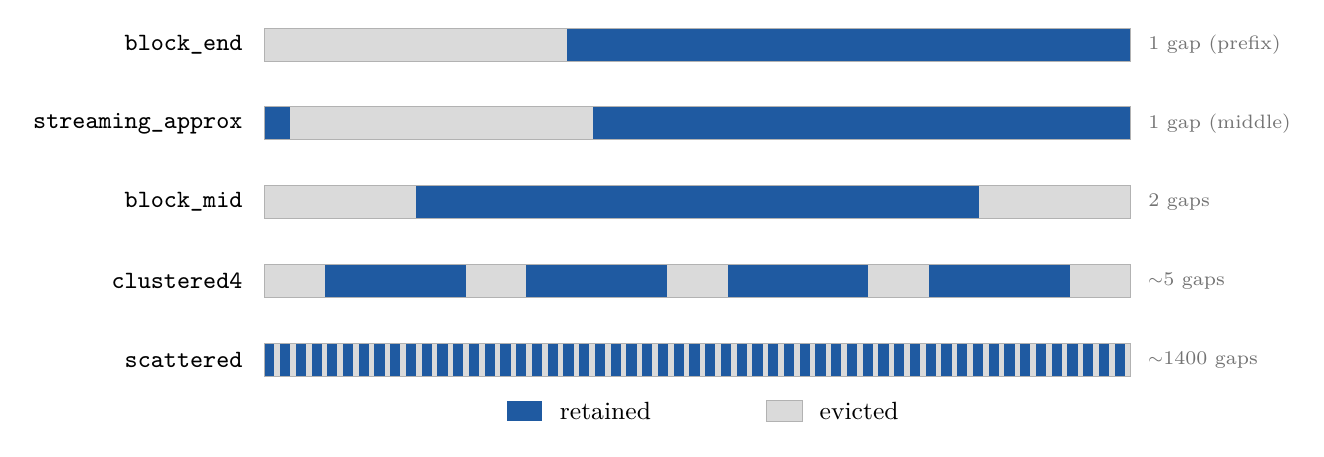
\begin{tikzpicture}
  % Layout constants (all in cm)
  \pgfmathsetmacro{\W}{11.0}   % bar width
  \pgfmathsetmacro{\H}{0.42}   % bar height
  \pgfmathsetmacro{\VS}{1.0}   % vertical spacing between row centres

  % Colours
  \definecolor{retcol}{RGB}{31,90,161}
  \definecolor{evtcol}{RGB}{218,218,218}

  % ── block\_end (row 4): evicted [0,35%], retained [35%,100%] ───────────────
  \fill[evtcol] (0,{4*\VS-\H/2}) rectangle ({\W*0.35},{4*\VS+\H/2});
  \fill[retcol] ({\W*0.35},{4*\VS-\H/2}) rectangle (\W,{4*\VS+\H/2});

  % ── streaming\_approx (row 3): sinks [0,3%] + evicted [3%,38%] + tail [38%,100%] ──
  % (sink width exaggerated from actual <0.1% for visibility)
  \fill[retcol] (0,{3*\VS-\H/2}) rectangle ({\W*0.03},{3*\VS+\H/2});
  \fill[evtcol] ({\W*0.03},{3*\VS-\H/2}) rectangle ({\W*0.38},{3*\VS+\H/2});
  \fill[retcol] ({\W*0.38},{3*\VS-\H/2}) rectangle (\W,{3*\VS+\H/2});

  % ── block\_mid (row 2): evicted [0,17.5%], retained [17.5%,82.5%], evicted [82.5%,100%] ──
  \fill[evtcol] (0,{2*\VS-\H/2}) rectangle ({\W*0.175},{2*\VS+\H/2});
  \fill[retcol] ({\W*0.175},{2*\VS-\H/2}) rectangle ({\W*0.825},{2*\VS+\H/2});
  \fill[evtcol] ({\W*0.825},{2*\VS-\H/2}) rectangle (\W,{2*\VS+\H/2});

  % ── clustered4 (row 1): 4 blocks × 16.25%, 5 gaps × 7% ────────────────────
  % Evicted segments
  \fill[evtcol] (0,{1*\VS-\H/2}) rectangle ({\W*0.07},{1*\VS+\H/2});
  \fill[evtcol] ({\W*0.2325},{1*\VS-\H/2}) rectangle ({\W*0.3025},{1*\VS+\H/2});
  \fill[evtcol] ({\W*0.465},{1*\VS-\H/2}) rectangle ({\W*0.535},{1*\VS+\H/2});
  \fill[evtcol] ({\W*0.6975},{1*\VS-\H/2}) rectangle ({\W*0.7675},{1*\VS+\H/2});
  \fill[evtcol] ({\W*0.93},{1*\VS-\H/2}) rectangle (\W,{1*\VS+\H/2});
  % Retained segments
  \fill[retcol] ({\W*0.07},{1*\VS-\H/2}) rectangle ({\W*0.2325},{1*\VS+\H/2});
  \fill[retcol] ({\W*0.3025},{1*\VS-\H/2}) rectangle ({\W*0.465},{1*\VS+\H/2});
  \fill[retcol] ({\W*0.535},{1*\VS-\H/2}) rectangle ({\W*0.6975},{1*\VS+\H/2});
  \fill[retcol] ({\W*0.7675},{1*\VS-\H/2}) rectangle ({\W*0.93},{1*\VS+\H/2});

  % ── scattered (row 0): dense comb schematic at 65% duty cycle ──────────────
  \fill[evtcol] (0,{-\H/2}) rectangle (\W,{\H/2});
  \pgfmathsetmacro{\NS}{55}
  \pgfmathsetmacro{\period}{\W/\NS}
  \pgfmathsetmacro{\sw}{\period*0.65}
  \foreach \i in {0,...,54} {
    \pgfmathsetmacro{\xs}{\i*\period}
    \fill[retcol] ({\xs},{-\H/2}) rectangle ({\xs+\sw},{\H/2});
  }

  % ── borders ────────────────────────────────────────────────────────────────
  \foreach \row in {0,1,2,3,4} {
    \draw[black!30, line width=0.3pt] (0,{\row*\VS-\H/2}) rectangle (\W,{\row*\VS+\H/2});
  }

  % ── row labels ─────────────────────────────────────────────────────────────
  \node[anchor=east, font=\small, inner sep=2pt] at (-0.2,{4*\VS}) {\texttt{block\_end}};
  \node[anchor=east, font=\small, inner sep=2pt] at (-0.2,{3*\VS}) {\texttt{streaming\_approx}};
  \node[anchor=east, font=\small, inner sep=2pt] at (-0.2,{2*\VS}) {\texttt{block\_mid}};
  \node[anchor=east, font=\small, inner sep=2pt] at (-0.2,{1*\VS}) {\texttt{clustered4}};
  \node[anchor=east, font=\small, inner sep=2pt] at (-0.2,0) {\texttt{scattered}};

  % ── gap-count annotations ──────────────────────────────────────────────────
  \node[anchor=west, font=\scriptsize, text=black!55, inner sep=2pt] at ({\W+0.15},{4*\VS}) {1 gap (prefix)};
  \node[anchor=west, font=\scriptsize, text=black!55, inner sep=2pt] at ({\W+0.15},{3*\VS}) {1 gap (middle)};
  \node[anchor=west, font=\scriptsize, text=black!55, inner sep=2pt] at ({\W+0.15},{2*\VS}) {2 gaps};
  \node[anchor=west, font=\scriptsize, text=black!55, inner sep=2pt] at ({\W+0.15},{1*\VS}) {$\sim$5 gaps};
  \node[anchor=west, font=\scriptsize, text=black!55, inner sep=2pt] at ({\W+0.15},0) {$\sim$1400 gaps};

  % ── legend ─────────────────────────────────────────────────────────────────
  \fill[retcol] ({\W*0.28},{-0.78}) rectangle ({\W*0.28+0.45},{-0.52});
  \node[anchor=west, font=\small] at ({\W*0.28+0.55},{-0.65}) {retained};
  \fill[evtcol] ({\W*0.58},{-0.78}) rectangle ({\W*0.58+0.45},{-0.52});
  \draw[black!30, line width=0.3pt] ({\W*0.58},{-0.78}) rectangle ({\W*0.58+0.45},{-0.52});
  \node[anchor=west, font=\small] at ({\W*0.58+0.55},{-0.65}) {evicted};

\end{tikzpicture}
\captionsetup{justification=centering}
\caption{Gap geometries used in the synthetic analysis (Table~\ref{tab:t2}). Each bar represents
\\the token sequence at $r = 0.65$ retention; blue = retained in KV cache, gray = evicted.
\\For \texttt{streaming\_approx}, the 4-token sink region at the head is exaggerated for visibility.}
\label{fig:gap-geometries}
\end{figure}

Each geometry evaluates the same retained position set under three
presentations:

\begin{itemize}
\tightlist
\item
  \textbf{Gapless}: positions gathered into a new, shorter, contiguous
  prompt --- compact RoPE positions, no enrichment from evicted context,
  no KV patching.
\item
  \textbf{Evicted}: full prefill over the complete prompt (enabling
  full-context enrichment), then post-prefill eviction; retained keys
  remain at their original RoPE positions. This is the mechanism used by
  SnapKV.
\end{itemize}

\begin{table}[H]
\centering
\small
\caption{Mean \(F_{\text{WTV}}\) (diagnostic) by gap geometry}
\label{tab:t2}
\begin{tabular}{@{}lllll@{}}
\toprule
Geometry & Gaps & Gapless & Evicted & ev/gl\\
\midrule
block\_end & 1 (prefix) & 0.149 & 0.544 & 3.6×\\
streaming\_approx & 1 (middle) & 0.146 & 0.081 & 0.55×\\
block\_mid & 2 & 0.644 & 0.640 & 1.0×\\
clustered4 & \textasciitilde5 & 0.610 & 0.624 & 1.0×\\
scattered & \textasciitilde1400 & 0.519 & 0.138 & 0.27×\\
\bottomrule
\\
\end{tabular}
\\Llama-3.1-8B, r = 0.65, 6 tasks, n = 20 per task.
\end{table}

Table~\ref{tab:t2} reveals several non-obvious patterns across the five geometries.

\begin{itemize}
\tightlist
\item
  \textbf{Block\_end geometry: attention sink loss.} A single large
  prefix gap causes severe damage: evicted (0.544) is 3.6× worse than
  gapless (0.149). The distinguishing factor is not the size of the
  evicted region but the loss of attention sink tokens at positions 0--3.
  Transformers develop a structural dependency on these early positions
  as anchor tokens where attention redistributes when no semantically
  relevant key is nearby. Block\_end eviction removes them entirely; the
  first KV entry in the compressed cache sits at position $T{-}M$, deep
  in the original sequence, and does not function as a natural sink. The
  result is destabilized attention during decode, visible in degenerate
  outputs such as repetitive loops.
\item
  \textbf{Streaming\_approx geometry: gap position determines outcome.}
  Adding just 4 sink tokens before the tail block shifts the single gap
  from the prefix boundary to the early-middle of the sequence, and the
  enrichment effect reverses completely: evicted (0.081) is 0.55× gapless
  (0.146) --- beneficial rather than damaging. The retained tokens now
  have both a sequence-initial anchor and the recency tail; the evicted
  middle content enriches their representations without creating the same
  systematic dependency on absent prefix context.
\item
  \textbf{Block\_mid and clustered4} show virtually no enrichment
  effect (1.0×). These geometries discard the recency tail, so their
  elevated gapless baselines reflect lower content informativeness rather
  than mechanism damage; within-geometry ratios are the interpretable
  signal.
\item
  \textbf{Scattered geometry: enrichment strongly beneficial (0.27×).}
  Uniformly-distributed positions with enrichment substantially
  outperform gapless (0.519 vs 0.138) --- enriched keys carry
  information about evicted context that compact-prompt construction
  cannot replicate, even at the same token budget.
\end{itemize}

The synthetic analysis isolates mechanism; task-level WTV variance in §4
reflects how well each geometry aligns with where relevant content actually
appears in a given task, which the content-blind synthetic cannot predict.

These results provide a mechanistic account of the clustering in §4.3.
SnapKV and PyramidKV share a scattered position geometry that
interacts strongly and favorably with enrichment (0.27×), explaining
why they form a tight group well above the remaining methods. Streaming
and Naive have a structurally similar geometry --- both retain sink
tokens plus a recency tail with a middle gap, approximating
streaming\_approx --- but Streaming undergoes post-prefill eviction
while Naive is prompt truncation. The WTV gap between them isolates the
enrichment effect: same structure, enrichment is the differentiator.




\hypertarget{why-compression-quality-appears-better}{%
\section{6. Why Compression Quality Appears Better Than It Actually Is}\label{why-compression-quality-appears-better}}

SnapKV and PyramidKV lead \(F_{\text{out}}\) across all retention rates
(Table~\ref{tab:t4}), and they also lead WTV faithfulness. The aggregate numbers,
however, conceal three structural effects that distort how well compression
quality is perceived to generalize.

\textbf{Enrichment and the short-answer advantage} (§6.1).  All post-prefill
eviction methods compute a complete, uncompressed prefill before eviction.
The retained KV pairs therefore carry representations formed under full-context
attention, making the compressed cache a higher-quality approximation of the
full model's state.  This enrichment inflates \(F_{\text{out}}\) on short-answer
tasks where a single correct word dominates the score.  WTV, being
teacher-forced on the full model's output sequence, is immune.

\textbf{Output-length effects} (§6.2).  The enrichment advantage
is concentrated on short outputs and dilutes on long ones as generated tokens
accumulate in the KV cache.  Splitting by output length reveals that
\(F_{\text{out}}\) gaps between methods are largely driven by short-answer
tasks; on long-form outputs the ranking shifts substantially, and WTV is a
more reliable guide to faithfulness at any length.

\textbf{Selection blind spot} (§6.3).  Attention-based
scoring produces a systematic positional bias: across models (Llama, Mistral),
the retained tokens form a bell curve peaking
near the middle of the sequence, with near-zero selection from the first 30\% of
the context.  This matters most for tasks where critical content is distributed
throughout the document rather than concentrated at the end---particularly
summarization, which has no retrieval target to focus attention and suffers the
largest WTV penalty as a result.

\hypertarget{first-token-advantage}{%
\subsection{6.1 Enrichment and the Short-Answer Advantage}\label{first-token-advantage}}

All post-prefill methods compute a complete, uncompressed prefill before
eviction. The retained KV pairs therefore carry representations formed
under full-context attention over the entire sequence --- each key and
value encodes cross-token interactions that would be absent if attention
had been restricted during prefill. This richer representation makes the
compressed cache a better approximation of the full model's state at every
decode position. Enrichment benefits both \(F_{\text{out}}\) and WTV: it
is a genuine quality improvement, not an artifact of evaluation procedure.

That enrichment --- not a structural guarantee about the first token --- is
what drives the short-answer \(F_{\text{out}}\) advantage is confirmed by
comparing SnapKV to the recompute-over-gaps variant introduced in §5.2
(Table~\ref{tab:rog}): both use identical attention-score selection at
the same retention budget; only the eviction point differs. The
recompute-over-gaps variant restricts attention \emph{during} prefill
rather than pruning the cache after it, so no enrichment accumulates.

\begin{table}[H]
\centering
\small
\caption{\(F_{\text{out}}\) by output-length category: enrichment diagnostic (Llama, 65\%)}
\label{tab:rog}
\begin{tabular}{@{}llll@{}}
\toprule
Method & Short-answer \(F_{\text{out}}\) & Long-form \(F_{\text{out}}\) & Gap\\
\midrule
Recompute-over-gaps & 56.1 & 50.2 & 6.0\\
SnapKV              & 87.7 & 54.7 & 33.0\\
\bottomrule
\end{tabular}

\center Llama-3.1-8B, 65\% retention. Short = reference output ≤\,90 words; Long = \textgreater{}90 words.
\end{table}

Table~\ref{tab:rog} shows the result: recompute-over-gaps is nearly flat
across output lengths (Gap=6.0), while SnapKV shows a steep 33.0-point
gradient. The same token selection rule with enrichment produces a
31-point short-answer advantage over the variant without it; on long-form
outputs both methods converge, consistent with enrichment being diluted
as generated tokens accumulate in the cache.

\hypertarget{output-length-effects}{%
\subsection{6.2 Output-Length Effects}\label{output-length-effects}}

Table~\ref{tab:t5} compares all methods by output-length category (Llama, 65\%),
with Naive as a reference. We set the threshold at 90 words because it
falls in a natural gap between two output regimes in LongBench: QA,
classification, and code-completion tasks have full-model mean outputs
of 14--48 words ($\geq$96\% of examples fall below 90 words), while
summarization tasks have means of 339--384 words ($\geq$86\% fall above).
NarrativeQA, Qasper, and SAMSum straddle the boundary with means near
80--90 words.
\begin{table}[H]
\centering
\small
\caption{\(F_{\text{out}}\) by output-length category (Llama, 65\%)}
\label{tab:t5}
\begin{tabular}{@{}llll@{}}
\toprule
Method & Short-answer \(F_{\text{out}}\) & Long-form \(F_{\text{out}}\)
& Gap\\
\midrule
PyramidKV & \textbf{88.1} & 55.5 & 32.6\\
SnapKV    & 87.7          & 54.7 & 33.0\\
Random    & 69.0          & 45.0 & 24.0\\
Streaming & 66.7          & 47.0 & 19.7\\
Naive     & 72.8          & \textbf{57.6} & 15.2\\
\bottomrule
\end{tabular}

\center Llama-3.1-8B, 65\% retention, all 16 tasks.
\\Short = full-model reference output ≤ 90 words (n=1155); Long =
\textgreater{} 90 words (n=445).
\end{table}

PyramidKV and SnapKV show nearly identical short-to-long drops
(\textasciitilde33 points), significantly larger than Random's (24.0), Naive's (15.2), and
Streaming's (19.7). The large gap for selection methods reflects enrichment quality (§\ref{first-token-advantage}):
their full-context prefill produces high-quality compressed KV pairs that generate
correct short answers. Random eviction's 19-point gap below the selection methods
(69.0 vs 87--88) confirms that selection quality matters; this advantage largely
disappears on long-form tasks where both converge to 45--55\% as enrichment dilutes.
Naive slightly leads all other methods on long-form \(F_{\text{out}}\)
(57.6 vs 55.5 and 54.7), and both selection methods achieve near-full-model
performance on single-token or short-phrase tasks: TriviaQA (Pyr: 97.0\%, Snap: 92.0\%),
PassageCount (96.4\%, 92.8\%), 2WikiMQA (95.6\%, 95.6\%), PassageRetrieval (93.8\%, 94.0\%).

\begin{table}[H]
\centering
\small
\caption{Mean \(F_{\text{WTV}}\) by output-length category (Llama-3.1-8B, 65\%)}
\label{tab:t6}
\begin{tabular}{@{}lll@{}}
\toprule
Method & Short \(F_{\text{WTV}}\) & Long \(F_{\text{WTV}}\)\\
\midrule
SnapKV    & 0.011          & 0.080\\
PyramidKV & \textbf{0.011} & \textbf{0.061}\\
Random    & 0.040          & 0.115\\
Streaming & 0.051          & 0.171\\
Naive     & 0.139          & 0.141\\
\bottomrule
\end{tabular}
\center
Llama-3.1-8B, 65\% retention, all 16 tasks.
\\Short = full-model reference output ≤ 90 words (n=1155); Long =
\textgreater{} 90 words (n=445).
\end{table}

Table~\ref{tab:t6} gives the WTV short/long breakdown.
SnapKV and PyramidKV are far more faithful than all other methods at
both output lengths, with PyramidKV slightly leading on long-form (0.061 vs 0.080
for SnapKV). Random eviction is 3.6$\times$ worse than SnapKV/Pyr on short outputs
(0.040 vs 0.011), confirming that intelligent selection contributes meaningfully to
WTV faithfulness even on short outputs. Streaming is 4.6$\times$ worse on short outputs and
2--3$\times$ worse on long outputs. Naive is nearly flat across lengths
(short 0.139, long 0.141) --- no enrichment benefit.

Enrichment explains the \(F_{\text{out}}\) pattern in Table~\ref{tab:t5}:
the high-quality compressed cache that enrichment produces drives correct
short answers for selection methods, while the advantage fades on longer
outputs as the enriched prompt KV entries are diluted by accumulated
generated tokens.

The practical implication is direct. Post-prefill eviction cannot reduce
TTFT, so any \(F_{\text{out}}\) advantage of SnapKV/PyramidKV is
concentrated precisely where latency savings are least: short exact-lookup
tasks where generation time is negligible and prefill dominates total cost.
On long-form tasks --- where TPT savings compound --- Naive's long-form
\(F_{\text{out}}\) (57.6\%) matches or exceeds SnapKV (54.7\%) and
PyramidKV (55.5\%) at 65\% retention, while delivering a 63\% TTFT reduction
(Table~\ref{tab:ttft}). SnapKV and PyramidKV lead meaningfully on WTV faithfulness
(§4.3) and on short-form \(F_{\text{out}}\), but the case for their superiority
on long-form generation tasks --- the workloads where compression saves the most
time --- rests on WTV faithfulness rather than output-text similarity.

\pgfplotsset{
  outlen/.style={
    width=0.48\textwidth, height=5.5cm,
    xmode=log, xmin=5, xmax=600,
    xtick={10,30,100,300}, xticklabels={10,30,100,300},
    xlabel={Full-model output (words)},
    grid=major, grid style={gray!20, line width=0.5pt},
    tick style={draw=none},
    every axis plot/.append style={line width=1.2pt, mark size=1.8pt},
    font=\small,
  }
}

\begin{figure}[H]
\centering
\begin{tikzpicture}
\begin{groupplot}[
  group style={group size=2 by 1, horizontal sep=1.4cm},
  outlen,
  ymin=25, ymax=100,
  ytick={40,60,80,100},
]
\nextgroupplot[
  title={65\% retention},
  ylabel={$F_{\text{out}}$ (\%)},
  legend to name={foutLenLeg},
  legend style={draw=none, font=\scriptsize, column sep=0.7em},
  legend columns=5,
]
\addplot[color=cSnap,   solid,        mark=*]
  coordinates{(8,89.5)(18,91.0)(21,92.3)(24,93.2)(26,94.8)(39,86.0)(69,74.8)(96,69.8)(258,52.6)(460,45.4)};
\addlegendentry{SnapKV}
\addplot[color=cPyr,    dashed,       mark=square*]
  coordinates{(8,92.1)(18,92.7)(21,93.4)(24,93.5)(26,94.1)(39,83.2)(69,77.1)(96,67.3)(258,54.7)(460,46.9)};
\addlegendentry{PyramidKV}
\addplot[color=cRandom, dash dot,     mark=diamond*]
  coordinates{(7,74.3)(18,67.5)(21,71.2)(23,74.7)(26,66.6)(43,71.0)(69,62.3)(95,53.3)(309,42.8)(441,39.8)};
\addlegendentry{Random}
\addplot[color=cStream, dotted,       mark=triangle*]
  coordinates{(8,71.8)(18,62.1)(21,68.0)(24,70.7)(26,72.0)(39,67.7)(69,60.0)(96,56.4)(258,46.7)(460,38.6)};
\addlegendentry{Streaming}
\addplot[color=cNaive,  dash dot dot, mark=o]
  coordinates{(8,64.7)(18,72.3)(21,76.1)(24,84.0)(26,76.3)(39,73.6)(69,63.1)(96,71.4)(258,54.8)(460,49.7)};
\addlegendentry{Naive}
%
\nextgroupplot[title={35\% retention}, yticklabels={}]
\addplot[color=cSnap,   solid,        mark=*]
  coordinates{(8,78.6)(18,77.0)(21,83.6)(24,85.7)(26,85.2)(39,72.6)(69,60.9)(96,53.5)(258,38.6)(460,36.1)};
\addplot[color=cPyr,    dashed,       mark=square*]
  coordinates{(8,78.8)(18,77.2)(21,84.3)(24,85.4)(26,85.4)(39,72.3)(69,60.9)(96,53.5)(258,39.0)(460,36.2)};
\addplot[color=cRandom, dash dot,     mark=diamond*]
  coordinates{(7,62.2)(18,53.5)(21,56.4)(23,63.0)(26,52.3)(43,56.1)(69,52.7)(95,46.7)(309,35.1)(441,36.1)};
\addplot[color=cStream, dotted,       mark=triangle*]
  coordinates{(8,56.1)(18,51.9)(21,56.8)(24,63.1)(26,66.4)(39,59.4)(69,51.2)(96,43.9)(258,35.7)(460,33.6)};
\addplot[color=cNaive,  dash dot dot, mark=o]
  coordinates{(8,37.7)(18,48.2)(21,48.2)(24,57.5)(26,53.0)(39,57.8)(69,48.8)(96,41.6)(258,38.1)(460,36.2)};
\end{groupplot}
\node[yshift=-2.1cm] at ($(group c1r1.south)!0.5!(group c2r1.south)$)
  {\pgfplotslegendfromname{foutLenLeg}};
\end{tikzpicture}
\caption{$F_{\text{out}}$ by full-model output length (Llama-3.1-8B, 16 tasks, $n \approx 155$/bin).}
\label{fig:fout-by-length}
\end{figure}

\begin{figure}[H]
\centering
\begin{tikzpicture}
\begin{groupplot}[
  group style={group size=2 by 1, horizontal sep=1.4cm},
  outlen,
  ymode=log,
  ymin=4e-3, ymax=0.6,
  ytick={1e-2,1e-1,1e0},
  yticklabels={$10^{-2}$,$10^{-1}$,$10^{0}$},
]
\nextgroupplot[
  title={65\% retention},
  ylabel={WTV},
  legend to name={wtvLenLeg},
  legend style={draw=none, font=\scriptsize, column sep=0.7em},
  legend columns=5,
]
\addplot[color=cSnap,   solid,        mark=*]
  coordinates{(7,0.0102)(19,0.0091)(21,0.0078)(24,0.0071)(27,0.0068)(48,0.0126)(84,0.0276)(98,0.0386)(375,0.1116)(444,0.0886)};
\addlegendentry{SnapKV}
\addplot[color=cPyr,    dashed,       mark=square*]
  coordinates{(7,0.0086)(19,0.0099)(21,0.0074)(24,0.0076)(27,0.0074)(48,0.0124)(84,0.0243)(98,0.0345)(375,0.0821)(444,0.0649)};
\addlegendentry{PyramidKV}
\addplot[color=cRandom, dash dot,     mark=diamond*]
  coordinates{(7,0.0365)(18,0.0414)(21,0.0398)(23,0.0314)(26,0.0329)(43,0.0450)(69,0.0470)(95,0.0661)(309,0.1496)(441,0.1159)};
\addlegendentry{Random}
\addplot[color=cStream, dotted,       mark=triangle*]
  coordinates{(7,0.0450)(19,0.0553)(21,0.0456)(24,0.0412)(27,0.0494)(48,0.0461)(84,0.0795)(98,0.0986)(375,0.2357)(444,0.1789)};
\addlegendentry{Streaming}
\addplot[color=cNaive,  dash dot dot, mark=o]
  coordinates{(7,0.1226)(19,0.1529)(21,0.1537)(24,0.1497)(27,0.1472)(48,0.1361)(84,0.1010)(98,0.1161)(375,0.1660)(444,0.1419)};
\addlegendentry{Naive}
%
\nextgroupplot[title={35\% retention}, yticklabels={}]
\addplot[color=cSnap,   solid,        mark=*]
  coordinates{(7,0.0284)(19,0.0256)(21,0.0215)(24,0.0214)(27,0.0215)(48,0.0314)(84,0.0658)(98,0.0851)(375,0.2196)(444,0.1678)};
\addplot[color=cPyr,    dashed,       mark=square*]
  coordinates{(7,0.0284)(19,0.0256)(21,0.0215)(24,0.0214)(27,0.0215)(48,0.0314)(84,0.0658)(98,0.0851)(375,0.2196)(444,0.1678)};
\addplot[color=cRandom, dash dot,     mark=diamond*]
  coordinates{(7,0.0731)(18,0.0732)(21,0.0725)(23,0.0599)(26,0.0582)(43,0.0814)(69,0.0832)(95,0.1189)(309,0.2554)(441,0.1969)};
\addplot[color=cStream, dotted,       mark=triangle*]
  coordinates{(7,0.0696)(19,0.0910)(21,0.0805)(24,0.0655)(27,0.0725)(48,0.0734)(84,0.1289)(98,0.1543)(375,0.3189)(444,0.2443)};
\addplot[color=cNaive,  dash dot dot, mark=o]
  coordinates{(7,0.1743)(19,0.2154)(21,0.2094)(24,0.1889)(27,0.1918)(48,0.2028)(84,0.1479)(98,0.1780)(375,0.2690)(444,0.2208)};
\end{groupplot}
\node[yshift=-2.1cm] at ($(group c1r1.south)!0.5!(group c2r1.south)$)
  {\pgfplotslegendfromname{wtvLenLeg}};
\end{tikzpicture}
\caption{$F_{\text{WTV}}$ by full-model output length (Llama-3.1-8B, 16 tasks, $n \approx 155$/bin).}
\label{fig:wtv-by-length}
\end{figure}

Figures~\ref{fig:fout-by-length} and \ref{fig:wtv-by-length} resolve both
metrics into ten equal-count decile bins spanning the full range of full-model
output lengths ($n \approx 160$ per bin), extending
Tables~\ref{tab:t5}--\ref{tab:base-wtv-shortlong} with a continuous view and adding Random eviction
(absent from those tables) and 35\% retention.  The $F_{\text{out}}$ panels show
that intelligent selection matters for short outputs but not long ones:
SnapKV and PyramidKV lead Random eviction by 14--18 points at the shortest
outputs (7 words: 89--92\% vs.\ 74\%), but the gap narrows to under 5 points
beyond 100 words and to under 2 points at 441 words.  Beyond roughly 100 words,
all methods --- including Streaming and Naive --- converge to similar
\(F_{\text{out}}\) values, and the convergence is nearly complete at 35\%
retention (spread of \textasciitilde3 points across all methods at 441 words,
vs.\ 41 points at 7 words).  At long outputs the information bottleneck of
compression itself dominates: no selection strategy can synthesize a faithful
long-form summary from 35\% of the document's tokens, and coverage breadth
matters as much as selection precision.  The WTV panels show the complementary
picture: SnapKV and PyramidKV achieve near-zero WTV on short outputs (enrichment
in full effect), while Random eviction is 3--4$\times$ worse at the same lengths
(0.037--0.041 vs.\ 0.009--0.010 for Snap/Pyr at 7 words), narrowing to
$\sim$1.3$\times$ beyond 300 words.  The mechanism is dilution: as generation
proceeds, newly decoded tokens accumulate in the KV cache alongside the
compressed prompt entries.  By step $t$, the cache holds $n_{\text{kept}}$
prompt tokens and $t$ generated tokens; once $t \gg n_{\text{kept}}$, attention
is dominated by the model's own prior outputs rather than the enriched prompt
context, and the quality difference between intelligent and random prompt
selection matters less.  Naive is nearly flat across the full length
distribution, confirming that truncation has no enrichment benefit.  The WTV
drop in the final bin (\textasciitilde441 words) is a task-composition effect:
those examples are drawn almost entirely from GovReport and MultiNews, whose
longest outputs consist of formulaic long-form prose where both models tend to
produce similarly structured text regardless of what was compressed, yielding
lower per-step distributional divergence than the shorter long-form outputs in
the preceding bin.


\hypertarget{selection-blind-spot}{%
\subsection{6.3 The Selection Blind Spot}\label{selection-blind-spot}}

Attention-based scoring selects the tokens the model attends to most during
prefill.  This seems like the right signal, yet both the WTV and \(F_{\text{out}}\)
results show that selection quality matters enormously.  A natural question is
\emph{what} the selection actually looks like: does attention concentrate on the
right tokens, or does it reflect a systematic bias in where the model looks?

Figure~\ref{fig:position-hist} answers this.  For each retained token, we record
its position as a fraction of the total sequence length, averaged over all layers
and attention heads.  Across 20 examples on five diverse LongBench tasks
(NarrativeQA, GovReport, HotpotQA, PassageRetrieval, TREC), the distribution is
not uniform: it forms a bell curve peaking at 45--65\% of the sequence, with
near-zero selection below 30\% and a narrow recency spike at the very end (the
fixed window).  The first quarter of every context---where background, definitions,
and framing typically appear---is almost entirely discarded.

The same bell curve appears on Mistral-7B-v0.3 (Figure~\ref{fig:position-hist}),
confirming the pattern is a property of the attention mechanism rather
than of any particular model architecture. At 35\% retention (right panel)
the peak shifts toward the sequence end and the recency spike grows, but
the first-quarter dead zone persists on both models.

\begin{figure}[H]
\centering
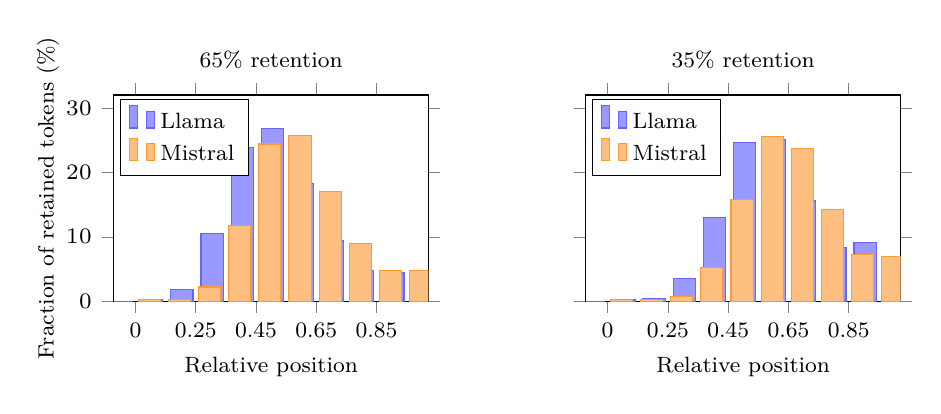
\begin{tikzpicture}
\begin{groupplot}[
  group style={group size=2 by 1, horizontal sep=2.0cm},
  width=0.46\linewidth,
  height=4.2cm,
  ybar,
  every axis/.append style={bar width=8pt},
  xlabel={Relative position},
  ymin=0, ymax=32,
  xtick={0.05,0.25,0.45,0.65,0.85},
  xticklabels={0,0.25,0.45,0.65,0.85},
  xticklabel style={font=\footnotesize},
  yticklabel style={font=\footnotesize},
  xlabel style={font=\footnotesize},
  ylabel style={font=\footnotesize,yshift=-4pt},
  tick align=outside,
  minor tick num=0,
  enlarge x limits=0.08,
  legend style={font=\footnotesize,at={(0.02,0.98)},anchor=north west},
  legend cell align=left,
]
\nextgroupplot[title={\footnotesize 65\% retention},
  ylabel={Fraction of retained tokens (\%)}]
\addplot[fill=blue!40,draw=blue!60] coordinates {
  (0.05,0.0)(0.15,0.2)(0.25,1.8)(0.35,10.5)(0.45,23.8)(0.55,26.8)(0.65,18.3)(0.75,9.4)(0.85,4.8)(0.95,4.5)
};
\addlegendentry{Llama}
\addplot[fill=orange!50,draw=orange!80] coordinates {
  (0.05,0.2)(0.15,0.2)(0.25,2.2)(0.35,11.7)(0.45,24.4)(0.55,25.7)(0.65,17.0)(0.75,9.0)(0.85,4.8)(0.95,4.8)
};
\addlegendentry{Mistral}
\nextgroupplot[title={\footnotesize 35\% retention}, yticklabels={}]
\addplot[fill=blue!40,draw=blue!60] coordinates {
  (0.05,0.0)(0.15,0.2)(0.25,0.4)(0.35,3.5)(0.45,13.0)(0.55,24.6)(0.65,25.1)(0.75,15.6)(0.85,8.4)(0.95,9.1)
};
\addlegendentry{Llama}
\addplot[fill=orange!50,draw=orange!80] coordinates {
  (0.05,0.2)(0.15,0.2)(0.25,0.8)(0.35,5.2)(0.45,15.8)(0.55,25.6)(0.65,23.7)(0.75,14.3)(0.85,7.2)(0.95,7.0)
};
\addlegendentry{Mistral}
\end{groupplot}
\end{tikzpicture}
\caption{SnapKV retained token positions as a fraction of sequence length,
  averaged over layers and heads (5 LongBench tasks, $n=20$, 10\%-wide bins).}
\label{fig:position-hist}
\end{figure}

The gaussian-bell experiment (§\ref{output-faithfulness}) makes the practical
consequence explicit: a stochastic selection that \emph{mimics the bell-curve shape}
but draws tokens randomly within it scores 53.5\% \(F_{\text{out}}\) at 65\%
retention---seven points below uniform random eviction (61.1\%) and 25 points below
SnapKV (78.7\%).  The bell shape is not what makes attention-based selection
valuable; the specific tokens chosen are.  The bias toward the middle of the sequence
is incidental to the scoring function, and on tasks where the critical content is
near the beginning---or distributed throughout---it actively hurts.

\label{summarization-hardest-case}%
The per-task breakdown in Appendix~B reveals a structural divide that aggregate numbers obscure: summarization tasks (GovReport, QMSum, MultiNews) show consistently high WTV across all methods, while retrieval and classification tasks reach near-zero WTV at the same retention rates. Table~\ref{tab:t-summ} makes the contrast explicit.

\begin{table}[H]
\centering
\small
\caption{WTV faithfulness on summarization vs.\ QA tasks (Llama-3.1-8B, 65\% retention, lower is better)}
\label{tab:t-summ}
\begin{tabular}{@{}lrrrr@{}}
\toprule
Task & Naive & Streaming & SnapKV & Pyr\\
\midrule
\multicolumn{5}{l}{\textit{Summarization}}\\
GovReport & 0.115 & 0.192 & 0.078 & \textbf{0.051}\\
QMSum     & 0.123 & 0.119 & 0.068 & \textbf{0.053}\\
MultiNews & 0.232 & 0.321 & 0.163 & \textbf{0.126}\\
\midrule
\multicolumn{5}{l}{\textit{Retrieval / classification}}\\
HotpotQA  & 0.159 & 0.054 & \textbf{0.008} & \textbf{0.008}\\
TriviaQA  & 0.138 & 0.021 & \textbf{0.001} & 0.002\\
TREC      & 0.137 & 0.007 & \textbf{0.001} & 0.002\\
\bottomrule
\end{tabular}

\center Llama-3.1-8B, 65\% retention. \textbf{Bold} = best per row.
\end{table}

On retrieval and classification tasks, SnapKV and PyramidKV achieve near-zero WTV
(0.001--0.008), more than 100$\times$ lower than Naive. On the three summarization tasks that
advantage shrinks to 1.5--2.5$\times$, and PyramidKV leads SnapKV by a meaningful margin
(GovReport: 0.051 vs.\ 0.078; MultiNews: 0.126 vs.\ 0.163).

The explanation is structural. Retrieval tasks have a localized answer; attention-guided selection
concentrates the retained cache around that answer's context. Summarization has no retrieval
target: the instruction is a generic ``summarize'' directive, so attention scores do not
preferentially identify any particular region of the document. Selection reverts to a positional
prior (Figures~\ref{fig:fout-by-length}--\ref{fig:wtv-by-length}
already show that selection and random eviction converge on long outputs), and the task requires
content from \emph{across} the document that is systematically evicted.

Naive truncation is comparatively more competitive on summarization. On HotpotQA and 2WikiMQA it
is 20$\times$ worse than SnapKV; on GovReport it is only 1.5$\times$ worse (0.115 vs.\ 0.078).
Truncation preserves the document's opening paragraphs intact, and for long reports the leading
section is disproportionately informative.

PyramidKV's advantage over SnapKV on summarization persists from 65\% to 50\%
(GovReport: 0.099 vs.\ 0.114 at 50\%) but vanishes at 35\%, where both methods score
identically on all three summarization tasks --- the same budget-collapse behaviour as in the
macro averages (§\ref{wtv-faithfulness-main-results}). The pyramid schedule assigns more
retained tokens to early and middle layers, where long-range cross-token integration is
richest; this aligns with what summarization demands, explaining why the advantage
exists but also why it collapses when per-layer budgets become too small to maintain a
gradient.

The practical implication is that the 16-task macro average used throughout §4 underweights
the summarization failure. SnapKV's aggregate WTV lead over Naive (0.030 vs.\ 0.139 at 65\%)
is driven almost entirely by near-zero scores on retrieval and classification tasks; on
GovReport and MultiNews the gap is modest, and at 35\% retention it disappears entirely. A
deployment whose workload is dominated by long-document summarization should not expect the
macro WTV ranking to hold.

\hypertarget{inference-performance}{%
\section{7. Inference Performance}\label{inference-performance}}

Compression is only worthwhile if it makes inference faster. We are theoretically sacrificing 
some quality of result in exchange for some gain in response time.  Generally there are two 
timings that are obvious to the user: how long does it take before I get any output and
how long does it take for the full answer.  Here we discuss how the compression methods
affect these and the factors that should be considered when calculating the trade-off between
speed and quality of result.

\subsection{7.1 Base Model Timing}\label{base-model-timing} 

There are typically two metrics that we use to measure the inference performance: 
\textbf{time to first token (TTFT)}, the wall-clock time from receiving a prompt to producing 
the first output token (dominated by the prefill pass), and \textbf{time per output token 
(TPT)}, the mean decode step time (dominated by KV cache memory bandwidth).
If we know the number of tokens in the response, the total inference
time can be calculated from those two numbers.

We will start by measuring the TTFT and TPT of the base model. 

\begin{table}[H]
\centering
\small
\caption{Mean TTFT and TPT by retention rate. Full-context baseline: 6425\,ms TTFT, 67.5\,ms/tok TPT.}
\label{tab:ttft}
\begin{tabular}{@{}llll@{}}
\toprule
Method & 65\% & 50\% & 35\%\\
\midrule
\multicolumn{4}{@{}l}{\textit{TTFT (ms)}}\\
Naive     & 2400 & 2082 & 1632\\
SnapKV    & 6621 & 6872 & 6834\\
Streaming & 6796 & 6750 & 6861\\
Pyr       & 6973 & 7245 & 7276\\
\midrule
\multicolumn{4}{@{}l}{\textit{TPT (ms/tok, all compressed methods)}}\\
All       & 53.5 & 48.4 & 43.6\\
\bottomrule
\end{tabular}
\center
Llama-3.1-8B fp16 on V100 GPU; 20 examples per task, averaged over\\2WikiMQA, MultifieldQA, Qasper, RepoBench-P, and TriviaQA.
\end{table}

Table~\ref{tab:ttft} shows mean TTFT by retention rate.
Naive cuts TTFT by 63--75\% by simply feeding the model a shorter
prompt. All post-prefill eviction methods incur overhead above the
full-context baseline: performing a full prefill over the uncompressed
prompt before pruning, each is consistently slower than the uncompressed
model at every retention rate. PyramidKV's layer-wise budget computation
adds 9--13\% overhead. SnapKV and Streaming use simpler post-prefill eviction steps and add less
overhead (+3--7\%), but both are consistently above full-context TTFT. No
KV-pruning method using post-prefill eviction can provide prefill savings:
the full prompt must be processed regardless.

The original online StreamingLLM design --- which
maintains a bounded cache continuously rather than performing a full
prefill --- would achieve TTFT closer to Naive than to the post-prefill
methods shown here, since prefill attention cost scales with the bounded
window size rather than the full context length.

Decode speed (TPT) improves for all compressed methods because
fewer retained tokens means a smaller KV cache to scan at each decode
step. At 65\% retention, mean TPT drops from 67.5 ms/tok (full) to
\textasciitilde54 ms/tok (\textasciitilde20\% faster) for all compressed
methods; at 35\% retention, all compressed methods reach
\textasciitilde44--48 ms/tok (\textasciitilde29--35\% faster).

\subsection{7.2 Instruct Model Timing at Extreme Budgets}\label{instruct-model-timing}

Table~\ref{tab:instruct-timing} gives mean wall-clock time per example at budgets~256 and~1024 for Llama-3.1-8B-Instruct, split by output-length category (short: full-model reference $\leq$10 words, $n=762$; long: $>$10 words, $n=838$).

\begin{table}[H]
\centering
\small
\caption{Mean wall-clock time per example by output-length category (Llama-3.1-8B-Instruct, V100)}
\label{tab:instruct-timing}
\begin{minipage}[t]{0.47\textwidth}
\centering
\textbf{Budget = 256}\\[4pt]
\begin{tabular}{@{}lrrr@{}}
\toprule
Method & Short (ms) & Long (ms) & Avg (ms)\\
\midrule
SnapKV    &  9372 & 11132 & 10294\\
PyramidKV &  9430 & 11355 & 10438\\
Streaming &  9772 & 11265 & 10554\\
Naive     &   725 &  4121 &  2504\\
Full      &  9666 & 16057 & 13013\\
\bottomrule
\end{tabular}
\end{minipage}
\hfill
\begin{minipage}[t]{0.47\textwidth}
\centering
\textbf{Budget = 1024}\\[4pt]
\begin{tabular}{@{}lrrr@{}}
\toprule
Method & Short (ms) & Long (ms) & Avg (ms)\\
\midrule
SnapKV    &  8855 & 11549 & 10266\\
PyramidKV &  8920 & 11880 & 10470\\
Streaming &  9269 & 11829 & 10610\\
Naive     &  1046 &  6258 &  3776\\
Full      &  9122 & 15918 & 12681\\
\bottomrule
\end{tabular}
\end{minipage}

\medskip
Avg = weighted mean over all examples ($n_{\text{short}}=762$, $n_{\text{long}}=838$).
Total time includes prefill and generation.
\end{table}

How faithfulness degrades with compression is not uniform across output types.
Short-answer tasks (QA, classification, code retrieval) and long-form tasks
(summarization, multi-hop reasoning) respond differently to the same compression method,
and the direction of that difference is reversed for WTV versus \(F_{\text{out}}\).

Table~\ref{tab:base-wtv-shortlong} shows the WTV short/long breakdown for the base
model at all three retention rates.
Short = full-model reference output $\leq$90~words ($n=1155$);
Long = $>$90~words ($n=445$).

\begin{table}[H]
\centering
\small
\captionsetup{justification=centering}
\caption{Mean \(F_{\text{WTV}}\) by output-length category (Llama-3.1-8B base)}
\label{tab:base-wtv-shortlong}
\begin{tabular}{@{}lrrrrrr@{}}
\toprule
& \multicolumn{2}{c}{65\%} & \multicolumn{2}{c}{50\%} & \multicolumn{2}{c}{35\%}\\
\cmidrule(lr){2-3}\cmidrule(lr){4-5}\cmidrule(lr){6-7}
Method & Short & Long & Short & Long & Short & Long\\
\midrule
SnapKV    & \textbf{0.011} & 0.080 & \textbf{0.019} & \textbf{0.116} & \textbf{0.030} & \textbf{0.158}\\
PyramidKV & \textbf{0.011} & \textbf{0.061} & 0.038 & 0.129 & \textbf{0.030} & \textbf{0.158}\\
Streaming & 0.051 & 0.171 & 0.066 & 0.205 & 0.082 & 0.239\\
Naive     & 0.139 & 0.141 & 0.154 & 0.182 & 0.191 & 0.222\\
\bottomrule
\end{tabular}
\center\smallskip
\textbf{Bold} = best per column.
All 16 tasks; short/long defined by full-model reference output length.
\end{table}

SnapKV and PyramidKV are the most faithful at every rate and output length.
The short/long gap in WTV is large for all selection methods: SnapKV has WTV
0.011 on short vs 0.080 on long at 65\% (7× ratio), consistent with enrichment quality being highest at early decode steps.
PyramidKV leads at 65\% (long 0.061 vs SnapKV 0.080);
SnapKV leads at 50\%, consistent with PyramidKV's pyramid budget collapsing
toward uniform allocation as compression tightens (§4.3). Both converge at 35\%.
Streaming WTV is roughly 3× worse on long outputs (0.171) than short (0.051)
at 65\%, consistent with block-end enrichment contamination accumulating over
longer generation. Naive WTV is nearly flat across short and long --- truncation
has no enrichment benefit and its errors distribute uniformly.

Table~\ref{tab:base-fout-shortlong} shows the \(F_{\text{out}}\) counterpart.

\begin{table}[H]
\centering
\small
\captionsetup{justification=centering}
\caption{\(F_{\text{out}}\) by output-length category (Llama-3.1-8B base)}
\label{tab:base-fout-shortlong}
\begin{tabular}{@{}lrrrrrr@{}}
\toprule
& \multicolumn{2}{c}{65\%} & \multicolumn{2}{c}{50\%} & \multicolumn{2}{c}{35\%}\\
\cmidrule(lr){2-3}\cmidrule(lr){4-5}\cmidrule(lr){6-7}
Method & Short & Long & Short & Long & Short & Long\\
\midrule
SnapKV    & \textbf{87.7} & 54.7 & \textbf{83.1} & 47.7 & \textbf{76.3} & 42.1\\
PyramidKV & \textbf{88.1} & \textbf{55.5} & 72.5 & 42.7 & 76.4 & 42.3\\
Streaming & 66.7 & 47.0 & 61.7 & \textbf{42.4} & 57.1 & \textbf{38.0}\\
Naive     & 72.8 & \textbf{57.6} & 55.6 & 42.9 & 50.0 & 38.8\\
\bottomrule
\end{tabular}
\center\smallskip
\textbf{Bold} = best per column.
All 16 tasks; short/long defined by full-model reference output length.
\end{table}

Here the direction flips: \(F_{\text{out}}\) is \emph{higher} on short outputs for
all selection methods (30+ point short/long gap for SnapKV/PyramidKV). Enrichment
inflates short-answer \(F_{\text{out}}\): the high-quality compressed cache drives
correct short answers, while the advantage fades over longer generation as
generated tokens dilute the enrichment effect.
Naive is the exception: its short/long \(F_{\text{out}}\) gap is small
(15 points at 65\%, near zero at 35\%), and Naive leads long-form
\(F_{\text{out}}\) at 65\% (57.6 vs 55.5 for the next-best).

Tables~\ref{tab:instruct-wtv-shortlong} and~\ref{tab:instruct-fout-shortlong}
give the same breakdown for the instruction-tuned model at budgets 256 and 1024.
The instruct model produces short answers regardless of compression: uncompressed,
it averages 3.9~words on HotpotQA and 4.5~words on NarrativeQA (vs.\ 21.9
and 80.6 for the base model), so nearly all instruct-model outputs fall in
the ``short'' category under any threshold. The \(F_{\text{out}}\) short/long gap
is large for all selection methods ($\approx$36 points for SnapKV/PyramidKV
at budget~256), driven by enrichment on single-word answers.
WTV shows the same direction: SnapKV WTV is 3× worse on long outputs than short
at budget~256 (0.405 vs 0.137), confirming that the metric advantage on short
outputs reflects enrichment quality, not a structural guarantee.

Table~\ref{tab:instruct-wtv-shortlong} gives the WTV breakdown by output-length category for the instruct model.

\begin{table}[H]
\centering
\small
\caption{Mean \(F_{\text{WTV}}\) by output-length category (Llama-3.1-8B-Instruct)}
\label{tab:instruct-wtv-shortlong}
\begin{minipage}[t]{0.47\textwidth}
\centering
\textbf{Budget = 256}\\[4pt]
\begin{tabular}{@{}lrrr@{}}
\toprule
Method & Short & Long & Long/Short\\
\midrule
SnapKV    & \textbf{0.137} & 0.405 & 3.0$\times$\\
PyramidKV & 0.139 & \textbf{0.403} & 2.9$\times$\\
Streaming & 0.249 & 0.455 & 1.8$\times$\\
Naive     & 0.543 & 0.508 & 0.9$\times$\\
\bottomrule
\end{tabular}
\end{minipage}
\hfill
\begin{minipage}[t]{0.47\textwidth}
\centering
\textbf{Budget = 1024}\\[4pt]
\begin{tabular}{@{}lrrr@{}}
\toprule
Method & Short & Long & Long/Short\\
\midrule
SnapKV    & \textbf{0.066} & 0.256 & 3.9$\times$\\
PyramidKV & 0.069 & \textbf{0.251} & 3.6$\times$\\
Streaming & 0.204 & 0.347 & 1.7$\times$\\
Naive     & 0.412 & 0.372 & 0.9$\times$\\
\bottomrule
\end{tabular}
\end{minipage}

\medskip
Long/Short = ratio of Long WTV to Short WTV; values below 1$\times$ indicate
lower WTV (better faithfulness) on long-form outputs than on short ones.
\end{table}

Table~\ref{tab:instruct-fout-shortlong} further breaks down \(F_{\text{out}}\) by output-length category at budgets~256 and~1024 (Llama only).

\begin{table}[H]
\centering
\small
\caption{\(F_{\text{out}}\) by output-length category (Llama-3.1-8B-Instruct)}
\label{tab:instruct-fout-shortlong}
\begin{minipage}[t]{0.47\textwidth}
\centering
\textbf{Budget = 256}\\[4pt]
\begin{tabular}{@{}lrrr@{}}
\toprule
Method & Short & Long & Gap\\
\midrule
SnapKV    & \textbf{91.0} & \textbf{54.7} & 36.3\\
PyramidKV & 90.5 & 53.5 & 37.1\\
Streaming & 72.1 & 41.5 & 30.6\\
Naive     & 23.8 & 25.8 & $-$2.0\\
\bottomrule
\end{tabular}
\end{minipage}
\hfill
\begin{minipage}[t]{0.47\textwidth}
\centering
\textbf{Budget = 1024}\\[4pt]
\begin{tabular}{@{}lrrr@{}}
\toprule
Method & Short & Long & Gap\\
\midrule
SnapKV    & \textbf{95.3} & \textbf{69.7} & 25.6\\
PyramidKV & 95.2 & 69.6 & 25.6\\
Streaming & 75.9 & 49.4 & 26.5\\
Naive     & 33.2 & 40.4 & $-$7.2\\
\bottomrule
\end{tabular}
\end{minipage}

\medskip
Gap = Short $-$ Long.  Naive bolded to highlight the comparison point.
\end{table}

Table~\ref{tab:t4} (Instruct columns) shows macro-averaged \(F_{\text{out}}\) at absolute token budgets on both instruct models (per-task breakdown in Appendices~C3--C4).

\subsection{7.3 Deployment Implications}\label{deployment-implications}

The timing results reveal a fundamental mismatch between where selection methods
are most accurate and where they actually save time. Post-prefill eviction methods
--- SnapKV, PyramidKV --- must process the full prompt before trimming, so TTFT is
never reduced below the full-context baseline; it is slightly higher
(Table~\ref{tab:ttft}). For short-answer tasks where TTFT dominates total latency,
selection methods deliver WTV faithfulness gains with no latency benefit. The
advantage exists precisely where compression provides no speedup.

The case for selection methods rests on long-form generation, where TPT savings
compound over many decode steps. At 35\% retention, compressed methods reach
\textasciitilde44--48\,ms/tok (\textasciitilde29--35\% faster than the
67.5\,ms/tok full-context rate), and this speedup grows proportionally with output
length. On long outputs, Naive provides a genuine throughput gain --- at
budget~=~256 on the instruct model, 4.1\,s versus 11.4\,s per example
(Table~\ref{tab:instruct-timing}) --- but with lower WTV faithfulness than selection
methods. For long-form generation where TPT savings are largest, SnapKV and
PyramidKV lead on WTV faithfulness and match Naive on long-form \(F_{\text{out}}\)
(§6.2): they are the right choice for applications where faithfulness to the full
model's behavior matters.

\hypertarget{conclusion}{%
\section{8. Conclusion}\label{conclusion}}

We introduced WTV faithfulness --- entropy-weighted total variation between
the full and compressed model's per-step token distributions --- as the
primary metric for evaluating KV cache compression fidelity, alongside
output faithfulness \(F_{\text{out}}\) as a human-readable behavioral anchor.
WTV is bounded in [0,\,1], making values interpretable across methods and
budgets without being distorted by isolated catastrophic divergences as KL is.
WTV is preferred over KL because KL's unbounded spikes from positional
displacement can distort method rankings; WTV suppresses these and
consistently recovers the ranking that output behavior corroborates.

On base models, scattered-selection methods (SnapKV, PyramidKV) are the most
faithful by WTV at every retention rate on both Llama-3.1-8B and Mistral-7B-v0.3,
with WTV values of 0.025--0.067 at 65--35\% retention vs 0.085--0.174 for
Streaming and 0.116--0.200 for Naive. The gap is explained by eviction geometry:
scattered retention interacts favorably with post-prefill value enrichment,
while block eviction contaminates retained values with expectations about the
missing prefix (§5). The same pattern holds at instruct budgets: SnapKV leads
at budgets 256 and 1024 on both Llama and Mistral instruct models.

The mechanism analysis in §5 has broader implications for compression
method design. The near-perfect faithfulness of scattered post-prefill
eviction (WTV 0.028) does not arise simply from retaining the right
tokens: the same tokens without a full prefill (SnapKV-Select, 0.120)
or with a full prefill but masked enrichment (recompute-over-gaps,
0.187) perform far worse. The decisive factor is that scattered
retention after a full prefill allows each retained KV pair to carry a
representation that attended over the entire original sequence,
including tokens immediately evicted afterward. Block eviction methods
are structurally excluded from this benefit: the gap geometry analysis (§5.3) shows that a single large prefix gap
incurs a 3.6× WTV penalty relative to the gapless case, while both
scattered and sink-plus-tail geometries produce beneficial enrichment
(0.27× and 0.55× respectively). The critical factor is not simply how
many tokens are retained but whether the gap structure creates a
systematic dependency on a single absent block. Researchers pursuing
block eviction should be aware that even a small sequence-initial
anchor (such as Streaming's sink tokens) substantially changes the
enrichment direction --- the disadvantage relative to scattered
selection is not merely retaining the wrong context window, but failing
to achieve the enrichment geometry that scattered selection provides as
a consequence of its token-selection policy.

Both metrics are needed to see through the enrichment effect: the full-context
prefill before eviction produces high-quality compressed KV pairs that inflate
short-answer \(F_{\text{out}}\) for selection methods regardless of how faithfully
they reproduce the full model's distributions at subsequent steps. WTV exposes
the same asymmetry --- SnapKV's WTV is 7× worse on long-form outputs than short
at 65\% --- and confirms that the aggregate advantage of selection methods in
\(F_{\text{out}}\) is partly a measurement artifact driven by LongBench's
short-answer tasks.
On long-form tasks, where reduced decode length would actually accelerate
inference, the \(F_{\text{out}}\) advantage of selection methods over Naive
truncation substantially narrows.

\hypertarget{references}{%
\section{References}\label{references}}

Ainslie, J., Lee-Thorp, J., de Jong, M., Zelaski, P., Sanghai, S., and
Su, Y. (2023). GQA: Training Generalized Multi-Query Transformer Models
by Interleaving Checkpoints. In \emph{Proceedings of EMNLP 2023}.
arXiv:2305.13245.

Bai, Y., Lv, X., Zhang, J., Lyu, H., Tang, J., Huang, Z., Du, Z., Liu,
X., Zeng, A., Hou, L., Dong, Y., Tang, J., and Li, J. (2023). LongBench:
A Bilingual, Multitask Benchmark for Long Context Understanding.
arXiv:2308.14508.

Cai, Z., Zhang, Y., Gao, B., Liu, Y., Li, Y., Liu, T., Lu, K., Xiong,
W., Dong, Y., Hu, J., and Xiao, W. (2024). PyramidKV: Dynamic KV Cache
Compression based on Pyramidal Information Funneling. arXiv:2406.02069.

Chen, A., Geh, R., Grover, A., et al.~(2025). The Pitfalls of KV Cache
Compression. arXiv:2510.00231.

Devoto, A., Jeblick, M., and Jégou, S. (2025). Expected Attention: KV
Cache Compression by Estimating Attention from Future Queries
Distribution. arXiv:2510.00636.

Dubey, A., Jauhri, A., Pandey, A., Kadian, A., Al-Dahle, A., Letman, A.,
Mathur, A., Schelten, A., Yang, A., Fan, A., et al.~(2024). The Llama 3
Herd of Models. arXiv:2407.21783.

Feng, Y., Lv, J., Cao, Y., Xie, X., and Zhou, S. K. (2025a). Ada-KV:
Optimizing KV Cache Eviction by Adaptive Budget Allocation for Efficient
LLM Inference. In \emph{Advances in Neural Information Processing
Systems (NeurIPS)}, 2025. arXiv:2407.11550.

Feng, Y., Lv, J., Guo, H., Cao, Y., Zhou, S. K., and Xie, X. (2025b).
CriticalKV: Optimizing KV Cache Eviction from an Output Perturbation
Perspective. In \emph{Proceedings of ICML 2026}. arXiv:2502.03805.

Fu, Y., Cai, Z., Asi, A., Xiong, W., Dong, Y., and Xiao, W. (2025). Not
All Heads Matter: A Head-Level KV Cache Compression Method with
Integrated Retrieval and Reasoning. In \emph{Proceedings of ICLR 2025}.
arXiv:2410.19258.

Guo, Z., Kamigaito, H., and Watanabe, T. (2024). Attention Score is not
All You Need for Token Importance Indicator in KV Cache Reduction: Value
Also Matters. In \emph{Proceedings of EMNLP 2024}. arXiv:2406.12335.

Jiang, A. Q., Sablayrolles, A., Mensch, A., Bamford, C., Chaplot, D. S.,
de las Casas, D., Bressand, F., Lengyel, G., Lample, G., Saulnier, L.,
Renard Lavaud, L., Lachaux, M.-A., Stock, P., Le Scao, T., Lavril, T.,
Wang, T., Lacroix, T., and El Sayed, W. (2023). Mistral 7B.
arXiv:2310.06825.

Li, Y., Huang, Y., Yang, B., Venkitesh, B., Locatelli, A., Ye, H., Cai,
T., Lewis, P., and Chen, D. (2024). SnapKV: LLM Knows What You are
Looking for Before Generation. arXiv:2404.14469.

Lin, C.-Y. (2004). ROUGE: A Package for Automatic Evaluation of
Summaries. In \emph{Proceedings of the Workshop on Text Summarization
Branches Out (WAS 2004)}.

Liu, Z., Desai, A., Liao, F., Wang, W., Xie, V., Xu, Z., Kyrillidis, A.,
and Shrivastava, A. (2023). Scissorhands: Exploiting the Persistence of
Importance Hypothesis for LLM KV Cache Compression at Test Time. In
\emph{Advances in Neural Information Processing Systems (NeurIPS)},
2023.

Papineni, K., Roukos, S., Ward, T., and Zhu, W.-J. (2002). BLEU: A
Method for Automatic Evaluation of Machine Translation. In
\emph{Proceedings of ACL 2002}.

Su, J., Lu, Y., Pan, S., Murtadha, A., Wen, B., and Liu, Y. (2024).
RoFormer: Enhanced Transformer with Rotary Position Embedding.
\emph{Neurocomputing}, 568, 127063. (arXiv:2104.09864.)

Tang, J., Zhao, Y., Zhu, K., Xiao, G., Kasikci, B., and Han, S. (2024).
Quest: Query-Aware Sparsity for Efficient Long-Context LLM Inference. In
\emph{Proceedings of ICML 2024}.

Wang, Z., Jin, B., Yu, Z., and Zhang, M. (2024). Model Tells You Where
to Merge: Adaptive KV Cache Merging for LLMs on Long-Context Tasks.
arXiv:2407.08454.

Zhang, Y., Du, Y., Luo, G., Zhong, Y., Zhang, Z., Liu, S., and Ji, R.
(2024). CaM: Cache Merging for Memory-efficient LLMs Inference. In
\emph{Proceedings of ICML 2024}. PMLR 235:58840--58850.

Xiao, G., Tang, J., Zuo, J., Guo, J., Yang, S., Tang, H., Fu, Y., and
Han, S. (2025). DuoAttention: Efficient Long-Context LLM Inference with
Retrieval and Streaming Heads. In \emph{Proceedings of ICLR 2025}.

Xiao, G., Tian, Y., Chen, B., Han, S., and Lewis, M. (2023). Efficient
Streaming Language Models with Attention Sinks. arXiv:2309.17453.
(Published at ICLR 2024.)

Zhang, T., Kishore, V., Wu, F., Weinberger, K. Q., and Artzi, Y. (2020).
BERTScore: Evaluating Text Generation with BERT. In \emph{Proceedings of
ICLR 2020}.

Zhang, Z., Sheng, Y., Zhou, T., Chen, T., Zheng, L., Cai, R., Song, Z.,
Tian, Y., Ré, C., Barrett, C., Wang, Z., and Chen, B. (2023). H2O:
Heavy-Hitter Oracle for Efficient Generative Inference of Large Language
Models. In \emph{Advances in Neural Information Processing Systems
(NeurIPS)}, 2023.


\clearpage
\hypertarget{appendix-b-ground-truth-accuracy-per-task-results}{%
\section{Appendix A: Ground-Truth Accuracy --- Per-Task
Results}\label{appendix-a-ground-truth-accuracy-per-task-results}}

\textbf{Tables A1a--A1c. Ground-truth accuracy per task, Llama-3.1-8B
(higher is better). Bold = best compressed method per row; ``Full'' is
the reference.}

\begin{table}[H]
\centering
\small
\caption*{Table A1a. 65\% retention.}
\begin{tabular}{@{}lrrrrrr@{}}
\toprule
Task & Full & Naive & Streaming & SnapKV & Pyr & Random\\
\midrule
    NarrativeQA\dag & 6.4 & 4.9 & 5.7 & 5.6 & 5.5 & \textbf{6.6}\\
    Qasper\dag & 12.7 & 10.2 & 9.5 & 11.3 & \textbf{11.8} & 10.7\\
    MultifieldQA & 27.8 & 27.0 & 26.3 & \textbf{30.2} & 29.4 & 30.1\\
    HotpotQA\dag & 11.2 & 9.6 & 9.0 & 9.9 & \textbf{10.2} & 9.7\\
    2WikiMQA\dag & 13.7 & 12.6 & 14.1 & 13.9 & 13.7 & \textbf{14.5}\\
    MuSiQue\dag & 7.3 & 7.0 & 5.8 & \textbf{7.2} & 7.1 & 6.8\\
    GovReport & 20.8 & 19.8 & 19.2 & 19.6 & \textbf{20.1} & 19.8\\
    QMSum\dag & 10.7 & \textbf{11.5} & 10.1 & 9.7 & 9.4 & 10.4\\
    MultiNews & 18.5 & 16.5 & 17.5 & \textbf{18.1} & 17.9 & 16.7\\
    TREC & 75.0 & 66.0 & 68.0 & \textbf{71.0} & \textbf{71.0} & 70.0\\
    TriviaQA & 17.8 & 17.3 & \textbf{17.5} & \textbf{17.5} & \textbf{17.5} & 17.3\\
    SAMSum & 15.9 & 16.5 & \textbf{17.1} & 16.2 & 16.3 & 15.8\\
    PassageCount\dag & 2.0 & 1.0 & \textbf{3.0} & \textbf{3.0} & \textbf{3.0} & \textbf{3.0}\\
    PassageRetrieval & 41.0 & 37.0 & 37.0 & \textbf{44.0} & \textbf{44.0} & 35.0\\
    LCC & 68.1 & 63.4 & 67.3 & 68.1 & \textbf{68.5} & 67.7\\
    RepoBench-P & 55.6 & 53.9 & 53.2 & 55.4 & \textbf{56.0} & 53.3\\
    \textbf{Average} & 25.3 & 23.4 & 23.8 & 25.0 & \textbf{25.1} & 24.2\\
\bottomrule
\end{tabular}
\end{table}

\begin{table}[H]
\centering
\small
\caption*{Table A1b. 50\% retention.}
\begin{tabular}{@{}lrrrrrr@{}}
\toprule
Task & Full & Naive & Streaming & SnapKV & Pyr & Random\\
\midrule
    NarrativeQA\dag & 6.4 & 5.7 & 5.5 & 6.7 & \textbf{6.8} & 4.4\\
    Qasper\dag & 12.7 & 8.6 & 9.1 & \textbf{11.1} & 9.8 & 9.7\\
    MultifieldQA & 27.8 & 23.0 & 25.3 & 29.2 & \textbf{29.5} & 28.0\\
    HotpotQA\dag & 11.2 & 8.9 & 9.6 & \textbf{9.7} & 9.6 & 9.4\\
    2WikiMQA\dag & 13.7 & 12.7 & 13.8 & \textbf{14.0} & 13.8 & 13.8\\
    MuSiQue\dag & 7.3 & 5.8 & 5.3 & \textbf{7.0} & 6.8 & 5.5\\
    GovReport & 20.8 & 19.5 & 19.0 & \textbf{20.0} & 19.5 & 19.8\\
    QMSum\dag & 10.7 & 9.5 & 9.3 & \textbf{9.7} & \textbf{9.7} & \textbf{9.7}\\
    MultiNews & 18.5 & 17.5 & \textbf{17.7} & 16.1 & 15.4 & 16.8\\
    TREC & 75.0 & 63.0 & 67.0 & \textbf{71.0} & 68.0 & 70.0\\
    TriviaQA & 17.8 & 17.4 & \textbf{17.5} & 17.4 & 17.3 & 16.9\\
    SAMSum & 15.9 & \textbf{17.7} & 17.6 & 16.1 & 17.6 & 16.0\\
    PassageCount\dag & 2.0 & 2.0 & \textbf{3.0} & \textbf{3.0} & \textbf{3.0} & \textbf{3.0}\\
    PassageRetrieval & 41.0 & 21.0 & 36.0 & \textbf{44.0} & 43.0 & 24.0\\
    LCC & 68.1 & 61.6 & 66.8 & 68.1 & 63.9 & \textbf{68.9}\\
    RepoBench-P & 55.6 & 51.4 & 53.8 & \textbf{55.7} & 52.8 & 53.9\\
    \textbf{Average} & 25.3 & 21.6 & 23.5 & \textbf{24.9} & 24.2 & 23.1\\
\bottomrule
\end{tabular}
\end{table}

\begin{table}[H]
\centering
\small
\caption*{Table A1c. 35\% retention.}
\begin{tabular}{@{}lrrrrrr@{}}
\toprule
Task & Full & Naive & Streaming & SnapKV & Pyr & Random\\
\midrule
    NarrativeQA\dag & 6.4 & \textbf{7.8} & 6.3 & 6.4 & 6.4 & 6.4\\
    Qasper\dag & 12.7 & 7.7 & 7.7 & \textbf{10.8} & \textbf{10.8} & 8.8\\
    MultifieldQA & 27.8 & 21.2 & 23.8 & \textbf{30.2} & 30.0 & 26.5\\
    HotpotQA\dag & 11.2 & \textbf{11.4} & 9.5 & 10.0 & 10.0 & 9.1\\
    2WikiMQA\dag & 13.7 & 11.0 & 12.4 & \textbf{14.6} & \textbf{14.6} & 12.2\\
    MuSiQue\dag & 7.3 & 4.7 & 5.0 & \textbf{6.5} & \textbf{6.5} & 5.1\\
    GovReport & 20.8 & 18.7 & 18.5 & 18.9 & \textbf{19.0} & 18.6\\
    QMSum\dag & 10.7 & 9.9 & 9.8 & \textbf{10.2} & \textbf{10.2} & 9.7\\
    MultiNews & 18.5 & \textbf{16.7} & 16.1 & 15.7 & 15.8 & 15.2\\
    TREC & 75.0 & 60.0 & 64.0 & \textbf{69.0} & \textbf{69.0} & 65.0\\
    TriviaQA & 17.8 & 17.3 & \textbf{18.4} & 17.4 & 17.4 & 17.7\\
    SAMSum & 15.9 & 17.6 & \textbf{18.5} & 17.3 & 17.3 & 17.3\\
    PassageCount\dag & 2.0 & \textbf{3.0} & \textbf{3.0} & \textbf{3.0} & \textbf{3.0} & \textbf{3.0}\\
    PassageRetrieval & 41.0 & 12.0 & 37.0 & \textbf{44.0} & \textbf{44.0} & 28.0\\
    LCC & 68.1 & 62.4 & 65.9 & 67.0 & 67.0 & \textbf{68.9}\\
    RepoBench-P & 55.6 & 50.6 & 53.9 & \textbf{55.1} & \textbf{55.1} & 52.2\\
    \textbf{Average} & 25.3 & 20.8 & 23.1 & \textbf{24.8} & \textbf{24.8} & 22.7\\
\bottomrule
\end{tabular}
\end{table}

\textbf{Tables A2a--A2c. Ground-truth accuracy per task, Mistral-7B-v0.3
(higher is better). Bold = best compressed method per row; Full is the
reference.}

\begin{table}[H]
\centering
\small
\caption*{Table A2a. 65\% retention.}
\begin{tabular}{@{}lrrrrrr@{}}
\toprule
Task & Full & Naive & Streaming & SnapKV & Pyr & Random\\
\midrule
    NarrativeQA\dag & 5.1 & 2.7 & \textbf{5.4} & 5.1 & 4.1 & 4.6\\
    Qasper\dag & 5.3 & 4.3 & \textbf{5.1} & \textbf{5.1} & 4.8 & 4.5\\
    MultifieldQA & 25.3 & 22.1 & 23.2 & 24.9 & 24.8 & \textbf{25.7}\\
    HotpotQA\dag & 10.5 & 10.6 & 9.9 & 10.7 & 10.6 & \textbf{11.5}\\
    2WikiMQA\dag & 11.5 & 9.8 & 11.2 & \textbf{11.7} & \textbf{11.7} & 11.2\\
    MuSiQue\dag & 5.1 & 3.9 & 3.9 & \textbf{5.1} & \textbf{5.1} & 4.7\\
    GovReport & 20.0 & 19.7 & 19.5 & 19.8 & \textbf{20.0} & 19.2\\
    QMSum\dag & 8.0 & \textbf{8.4} & 8.2 & 7.9 & 7.9 & 7.7\\
    MultiNews & 18.1 & 17.2 & 17.1 & 17.2 & 17.3 & \textbf{17.5}\\
    TREC & 72.0 & 67.0 & 69.0 & 70.0 & \textbf{71.0} & \textbf{71.0}\\
    TriviaQA & 23.1 & 24.2 & \textbf{24.6} & 23.4 & 23.3 & 24.5\\
    SAMSum & 16.9 & 17.8 & \textbf{18.6} & 17.9 & 18.1 & 17.5\\
    PassageCount\dag & 1.0 & \textbf{3.0} & 1.0 & 1.0 & 1.0 & 2.0\\
    PassageRetrieval & 39.0 & 26.0 & 30.0 & \textbf{39.0} & \textbf{39.0} & 28.0\\
    LCC & 62.9 & 60.2 & 62.4 & \textbf{63.2} & \textbf{63.2} & 62.6\\
    RepoBench-P & 53.9 & \textbf{54.4} & 54.0 & 54.1 & 54.0 & 54.1\\
    \textbf{Average} & 23.6 & 22.0 & 22.7 & \textbf{23.5} & 23.5 & 22.9\\
\bottomrule
\end{tabular}
\end{table}

\begin{table}[H]
\centering
\small
\caption*{Table A2b. 50\% retention.}
\begin{tabular}{@{}lrrrrrr@{}}
\toprule
Task & Full & Naive & Streaming & SnapKV & Pyr & Random\\
\midrule
    NarrativeQA\dag & 5.1 & 4.7 & 4.5 & \textbf{5.1} & 5.0 & 4.4\\
    Qasper\dag & 5.3 & 4.5 & 4.5 & \textbf{4.7} & 4.4 & 4.4\\
    MultifieldQA & 25.3 & 18.0 & 23.4 & 25.0 & \textbf{25.6} & 24.6\\
    HotpotQA\dag & 10.5 & 10.3 & \textbf{10.9} & 10.5 & 10.7 & 10.3\\
    2WikiMQA\dag & 11.5 & 9.5 & 11.4 & 11.4 & 11.8 & \textbf{12.1}\\
    MuSiQue\dag & 5.1 & 4.7 & 4.1 & \textbf{5.3} & 5.1 & 4.6\\
    GovReport & 20.0 & 19.1 & 18.5 & \textbf{19.5} & 18.4 & 18.6\\
    QMSum\dag & 8.0 & 8.0 & \textbf{8.1} & 7.6 & 7.5 & 7.8\\
    MultiNews & 18.1 & \textbf{16.7} & 16.4 & 16.4 & 15.6 & 16.5\\
    TREC & 72.0 & 62.0 & 66.0 & \textbf{70.0} & 67.0 & \textbf{70.0}\\
    TriviaQA & 23.1 & 26.1 & 24.1 & 23.9 & 23.8 & \textbf{27.1}\\
    SAMSum & 16.9 & 17.3 & 17.2 & 17.1 & \textbf{19.1} & 17.2\\
    PassageCount\dag & 1.0 & 3.0 & 1.0 & 1.0 & 1.0 & \textbf{5.0}\\
    PassageRetrieval & 39.0 & 23.0 & 26.0 & \textbf{39.0} & 38.0 & 27.0\\
    LCC & 62.9 & 58.9 & \textbf{64.8} & 62.9 & 60.1 & 61.3\\
    RepoBench-P & 53.9 & 52.2 & 53.3 & \textbf{54.1} & 53.8 & 53.5\\
    \textbf{Average} & 23.6 & 21.1 & 22.1 & \textbf{23.3} & 22.9 & 22.8\\
\bottomrule
\end{tabular}
\end{table}

\begin{table}[H]
\centering
\small
\caption*{Table A2c. 35\% retention.}
\begin{tabular}{@{}lrrrrrr@{}}
\toprule
Task & Full & Naive & Streaming & SnapKV & Pyr & Random\\
\midrule
    NarrativeQA\dag & 5.1 & 3.9 & 4.7 & \textbf{5.1} & \textbf{5.1} & 3.6\\
    Qasper\dag & 5.3 & 4.0 & 4.1 & \textbf{4.9} & 4.8 & 3.9\\
    MultifieldQA & 25.3 & 18.2 & 19.4 & \textbf{25.1} & \textbf{25.1} & 22.6\\
    HotpotQA\dag & 10.5 & 11.0 & \textbf{11.3} & 10.4 & 10.4 & 10.9\\
    2WikiMQA\dag & 11.5 & 11.6 & \textbf{12.5} & 11.2 & 11.2 & 11.4\\
    MuSiQue\dag & 5.1 & 4.6 & 3.6 & \textbf{5.2} & \textbf{5.2} & 3.9\\
    GovReport & 20.0 & \textbf{18.6} & 18.0 & \textbf{18.6} & \textbf{18.6} & 18.4\\
    QMSum\dag & 8.0 & 7.8 & \textbf{8.1} & 7.8 & 7.8 & 8.0\\
    MultiNews & 18.1 & \textbf{16.5} & 15.1 & 15.7 & 15.7 & 15.7\\
    TREC & 72.0 & 60.0 & 62.0 & 66.0 & 66.0 & \textbf{69.0}\\
    TriviaQA & 23.1 & 25.3 & 25.8 & 23.7 & 23.7 & \textbf{28.4}\\
    SAMSum & 16.9 & 17.2 & \textbf{18.4} & 17.8 & 17.8 & 17.2\\
    PassageCount\dag & 1.0 & 3.0 & 1.0 & 1.0 & 1.0 & \textbf{5.0}\\
    PassageRetrieval & 39.0 & 15.0 & 22.0 & \textbf{39.0} & \textbf{39.0} & 18.0\\
    LCC & 62.9 & 57.4 & \textbf{63.4} & 62.3 & 62.3 & 60.9\\
    RepoBench-P & 53.9 & 49.5 & 52.3 & \textbf{53.7} & \textbf{53.7} & 52.2\\
    \textbf{Average} & 23.6 & 20.2 & 21.4 & \textbf{23.0} & 23.0 & 21.8\\
\bottomrule
\end{tabular}
\end{table}

\clearpage
\subsection*{Instruction-tuned models (budgets 256 and 1024 tokens)}


\textbf{Table A3a. Ground-truth accuracy (\%) per task, Llama-3.1-8B-Instruct,
budget = 256 tokens (higher is better). ``Full'' is the reference and is not bolded.
Bold = best compressed method per row.
$n = 100$ per task. \(\dagger\) = low full-context score; results noisier.}

\begin{table}[H]
\centering
\small
\begin{tabular}{@{}lrrrrrrr@{}}
\toprule
Task & Full & Naive & Streaming & SnapKV & Pyr & Random\\
\midrule
    NarrativeQA\dagger & 27.0 & 9.8 & 20.8 & \textbf{26.5} & 25.1 & 20.9\\
    Qasper\dagger & 42.4 & 11.4 & 23.3 & 34.5 & \textbf{38.1} & 24.2\\
    MultifieldQA & 45.3 & 18.7 & 32.0 & \textbf{45.2} & 44.6 & 34.3\\
    HotpotQA\dagger & 47.9 & 21.9 & 39.7 & \textbf{47.2} & 46.7 & 40.6\\
    2WikiMQA\dagger & 48.9 & 10.8 & 43.7 & 47.0 & \textbf{47.9} & 41.5\\
    MuSiQue\dagger & 22.6 & 4.5 & 16.5 & 21.3 & \textbf{21.8} & 17.3\\
    GovReport & 21.5 & 15.1 & 16.4 & 18.3 & \textbf{18.4} & 16.5\\
    QMSum\dagger & 19.2 & 15.9 & 18.0 & \textbf{18.9} & 18.8 & 18.7\\
    MultiNews & 18.2 & 15.3 & 14.9 & 15.7 & 15.3 & \textbf{15.7}\\
    TREC & 18.0 & 6.0 & 5.0 & 19.0 & \textbf{26.0} & 3.0\\
    TriviaQA & 75.4 & 43.8 & 72.8 & 75.7 & \textbf{76.0} & 71.4\\
    SAMSum & 14.5 & \textbf{24.9} & 16.0 & 14.8 & 14.0 & 15.5\\
    PassageCount\dagger & 3.0 & 0.0 & \textbf{3.0} & 3.0 & 3.0 & 3.0\\
    PassageRetrieval & 67.0 & 3.0 & 63.0 & \textbf{67.0} & 67.0 & 62.0\\
    LCC & 19.8 & \textbf{34.9} & 20.7 & 19.7 & 19.5 & 20.6\\
    RepoBench-P & 17.0 & \textbf{33.9} & 17.3 & 17.1 & 16.6 & 16.6\\
    \textbf{Average} & 31.7 & 16.9 & 26.4 & 30.7 & \textbf{31.2} & 26.4\\
\bottomrule
\end{tabular}
\end{table}


\textbf{Table A3b. Ground-truth accuracy (\%) per task, Llama-3.1-8B-Instruct,
budget = 1024 tokens (higher is better). ``Full'' is the reference and is not bolded.
Bold = best compressed method per row. $n = 100$ per task.
\(\dagger\) = low full-context score; results noisier.}

\begin{table}[H]
\centering
\small
\begin{tabular}{@{}lrrrrrrr@{}}
\toprule
Task & Full & Naive & Streaming & SnapKV & Pyr & Random\\
\midrule
    NarrativeQA\dagger & 27.0 & 12.6 & 23.0 & 25.2 & \textbf{26.4} & 24.1\\
    Qasper\dagger & 42.4 & 16.3 & 25.7 & 41.0 & \textbf{41.4} & 36.3\\
    MultifieldQA & 45.3 & 29.2 & 34.9 & 45.3 & \textbf{46.0} & 41.6\\
    HotpotQA\dagger & 47.9 & 26.7 & 43.0 & \textbf{48.2} & 47.7 & 42.8\\
    2WikiMQA\dagger & 48.9 & 26.6 & 45.6 & 48.2 & \textbf{49.2} & 43.9\\
    MuSiQue\dagger & 22.6 & 11.8 & 15.6 & 22.3 & 21.6 & \textbf{23.6}\\
    GovReport & 21.5 & 18.1 & 17.9 & 19.3 & \textbf{19.4} & 18.2\\
    QMSum\dagger & 19.2 & 17.0 & 18.0 & 19.1 & \textbf{19.2} & 18.7\\
    MultiNews & 18.2 & 17.7 & 17.7 & 17.9 & \textbf{18.0} & 17.8\\
    TREC & 18.0 & 15.0 & 4.0 & 20.0 & 21.0 & \textbf{22.0}\\
    TriviaQA & 75.4 & 61.7 & 75.5 & \textbf{76.0} & 75.7 & 74.8\\
    SAMSum & 14.5 & \textbf{16.0} & 15.9 & 14.4 & 14.7 & 14.4\\
    PassageCount\dagger & 3.0 & 2.0 & \textbf{3.0} & 3.0 & 3.0 & 3.0\\
    PassageRetrieval & 67.0 & 10.0 & 54.0 & \textbf{67.0} & 67.0 & 60.0\\
    LCC & 19.8 & \textbf{20.6} & 20.1 & 19.9 & 19.5 & 19.9\\
    RepoBench-P & 17.0 & \textbf{20.5} & 17.1 & 16.9 & 16.8 & 17.4\\
    \textbf{Average} & 31.7 & 20.1 & 26.9 & 31.5 & \textbf{31.6} & 29.9\\
\bottomrule
\end{tabular}
\end{table}



\textbf{Table A4a. Ground-truth accuracy (\%) per task, Mistral-7B-Instruct-v0.3,
budget = 256 tokens (higher is better). ``Full'' is the reference and is not bolded.
Bold = best compressed method per row.
$n = 100$ per task. \(\dagger\) = low full-context score; results noisier.}

\nopagebreak
\begin{table}[H]
\centering
\small
\begin{tabular}{@{}lrrrrrrr@{}}
\toprule
Task & Full & Naive & Streaming & SnapKV & Pyr & Random\\
\midrule
    NarrativeQA\dagger & 22.2 & 6.8 & 15.2 & 19.8 & \textbf{20.5} & 16.5\\
    Qasper\dagger & 38.5 & 8.9 & 20.2 & 31.7 & \textbf{31.7} & 22.5\\
    MultifieldQA & 42.2 & 17.6 & 27.8 & \textbf{40.6} & 40.2 & 26.8\\
    HotpotQA\dagger & 42.3 & 21.0 & 31.0 & \textbf{41.8} & 41.8 & 32.0\\
    2WikiMQA\dagger & 40.3 & 13.9 & 34.4 & 37.3 & \textbf{37.4} & 33.0\\
    MuSiQue\dagger & 15.7 & 6.8 & 12.9 & 17.8 & \textbf{18.4} & 12.1\\
    GovReport & 22.6 & 15.0 & 14.9 & \textbf{18.5} & 17.7 & 15.3\\
    QMSum\dagger & 19.5 & 15.9 & 17.6 & 18.6 & \textbf{19.0} & 17.7\\
    MultiNews & 18.6 & 15.1 & 15.0 & \textbf{16.4} & 16.3 & 16.0\\
    TREC & 33.0 & \textbf{36.0} & 16.0 & 34.0 & 36.0 & 19.0\\
    TriviaQA & 81.8 & 41.4 & 77.7 & 80.1 & \textbf{83.3} & 75.3\\
    SAMSum & 40.4 & 28.5 & 33.3 & 38.9 & \textbf{39.3} & 33.4\\
    PassageCount\dagger & 3.0 & 1.0 & \textbf{4.0} & 2.0 & 1.0 & 3.0\\
    PassageRetrieval & 56.0 & 3.0 & 15.0 & 56.0 & \textbf{57.0} & 16.0\\
    LCC & 18.1 & 16.7 & \textbf{18.9} & 18.1 & 18.2 & 18.3\\
    RepoBench-P & 30.0 & 19.6 & 27.5 & \textbf{29.9} & 27.9 & 28.2\\
    \textbf{Average} & 32.8 & 16.7 & 23.8 & 31.3 & \textbf{31.6} & 24.1\\
\bottomrule
\end{tabular}
\end{table}


\textbf{Table A4b. Ground-truth accuracy (\%) per task,
Mistral-7B-Instruct-v0.3, budget = 1024 tokens (higher is better).
Full = uncompressed model. Bold = best compressed method per row.
†Long-context task. $n = 100$ per task.}

\begin{table}[H]
\centering
\small
\begin{tabular}{@{}lrrrrrrr@{}}
\toprule
Task & Full & Naive & Streaming & SnapKV & Pyr & Random\\
\midrule
    NarrativeQA\dagger & 22.2 & 9.2 & 17.6 & \textbf{23.4} & 22.4 & 21.1\\
    Qasper\dagger & 38.5 & 13.3 & 24.9 & \textbf{34.3} & 33.6 & 28.6\\
    MultifieldQA & 42.2 & 27.6 & 31.0 & \textbf{42.5} & 42.4 & 37.0\\
    HotpotQA\dagger & 42.3 & 25.1 & 37.7 & \textbf{42.6} & 42.2 & 40.3\\
    2WikiMQA\dagger & 40.3 & 21.7 & 35.2 & 37.6 & \textbf{39.1} & 35.5\\
    MuSiQue\dagger & 15.7 & 9.5 & 11.7 & \textbf{16.4} & 14.8 & 13.0\\
    GovReport & 22.6 & 17.6 & 17.6 & \textbf{19.5} & 18.9 & 18.7\\
    QMSum\dagger & 19.5 & 17.4 & 17.9 & 19.1 & \textbf{19.4} & 18.6\\
    MultiNews & 18.6 & 17.8 & \textbf{18.2} & 17.9 & 18.1 & 18.2\\
    TREC & 33.0 & \textbf{38.0} & 18.0 & 33.0 & 30.0 & 22.0\\
    TriviaQA & 81.8 & 60.2 & 83.0 & 81.5 & \textbf{84.1} & 79.4\\
    SAMSum & 40.4 & 32.6 & 37.7 & 40.6 & \textbf{40.7} & 36.7\\
    PassageCount\dagger & 3.0 & 0.0 & \textbf{3.0} & 3.0 & 2.0 & 1.0\\
    PassageRetrieval & 56.0 & 6.0 & 16.0 & 56.0 & \textbf{57.0} & 23.0\\
    LCC & 18.1 & 17.5 & 18.8 & 18.3 & \textbf{18.8} & 18.3\\
    RepoBench-P & 30.0 & 20.2 & 27.8 & \textbf{30.2} & 29.4 & 27.9\\
    \textbf{Average} & 32.8 & 20.9 & 26.0 & \textbf{32.2} & 32.1 & 27.4\\
\bottomrule
\end{tabular}
\end{table}


\clearpage
\hypertarget{appendix-b-wtv-faithfulness-per-task-results}{%
\section{Appendix B: WTV Faithfulness --- Per-Task
Results}\label{appendix-b-wtv-faithfulness-per-task-results}}

\textbf{Tables B1a--B1c. WTV faithfulness (\(F_{\text{WTV}}\)) per task, Llama-3.1-8B
(lower is better). Bold = best per row.}

\begin{table}[H]
\centering
\small
\caption*{Table B1a. 65\% retention.}
\begin{tabular}{@{}lrrrrr@{}}
\toprule
Task & Naive & Streaming & SnapKV & Pyr & Random\\
\midrule
    NarrativeQA\dag & 0.082 & 0.066 & 0.017 & \textbf{0.015} & 0.050\\
    Qasper\dag & 0.161 & 0.115 & 0.054 & \textbf{0.045} & 0.093\\
    MultifieldQA & 0.131 & 0.102 & 0.025 & \textbf{0.019} & 0.076\\
    HotpotQA\dag & 0.159 & 0.054 & \textbf{0.008} & 0.008 & 0.032\\
    2WikiMQA\dag & 0.172 & 0.049 & 0.009 & \textbf{0.007} & 0.030\\
    MuSiQue\dag & 0.163 & 0.054 & \textbf{0.008} & 0.009 & 0.032\\
    GovReport & 0.115 & 0.192 & 0.078 & \textbf{0.051} & 0.126\\
    QMSum\dag & 0.123 & 0.119 & 0.068 & \textbf{0.052} & 0.079\\
    MultiNews & 0.232 & 0.321 & 0.163 & \textbf{0.126} & 0.205\\
    TREC & 0.137 & 0.007 & \textbf{0.001} & 0.002 & 0.005\\
    TriviaQA & 0.138 & 0.021 & \textbf{0.001} & 0.002 & 0.024\\
    SAMSum & 0.065 & 0.062 & 0.020 & \textbf{0.019} & 0.045\\
    PassageCount\dag & 0.122 & 0.009 & \textbf{0.001} & 0.002 & 0.007\\
    PassageRetrieval & 0.184 & 0.032 & \textbf{0.002} & 0.002 & 0.021\\
    LCC & 0.140 & 0.076 & \textbf{0.017} & 0.019 & 0.066\\
    RepoBench-P & 0.105 & 0.074 & \textbf{0.011} & 0.013 & 0.077\\
    \textbf{Average} & 0.139 & 0.085 & 0.030 & \textbf{0.025} & 0.061\\
\bottomrule
\end{tabular}
\end{table}

\begin{table}[H]
\centering
\small
\caption*{Table B1b. 50\% retention.}
\begin{tabular}{@{}lrrrrr@{}}
\toprule
Task & Naive & Streaming & SnapKV & Pyr & Random\\
\midrule
    NarrativeQA\dag & 0.104 & 0.080 & \textbf{0.028} & 0.110 & 0.067\\
    Qasper\dag & 0.210 & 0.165 & \textbf{0.083} & 0.122 & 0.128\\
    MultifieldQA & 0.150 & 0.131 & \textbf{0.039} & 0.056 & 0.103\\
    HotpotQA\dag & 0.159 & 0.063 & \textbf{0.012} & 0.025 & 0.045\\
    2WikiMQA\dag & 0.194 & 0.068 & \textbf{0.018} & 0.029 & 0.043\\
    MuSiQue\dag & 0.156 & 0.065 & \textbf{0.013} & 0.024 & 0.044\\
    GovReport & 0.158 & 0.224 & 0.114 & \textbf{0.099} & 0.166\\
    QMSum\dag & 0.156 & 0.154 & 0.096 & \textbf{0.089} & 0.106\\
    MultiNews & 0.292 & 0.363 & 0.231 & \textbf{0.224} & 0.273\\
    TREC & 0.173 & 0.010 & \textbf{0.003} & 0.007 & 0.008\\
    TriviaQA & 0.169 & 0.035 & \textbf{0.002} & 0.013 & 0.033\\
    SAMSum & 0.073 & 0.078 & \textbf{0.032} & 0.062 & 0.064\\
    PassageCount\dag & 0.120 & 0.012 & \textbf{0.002} & 0.005 & 0.010\\
    PassageRetrieval & 0.191 & 0.041 & \textbf{0.004} & 0.006 & 0.029\\
    LCC & 0.164 & 0.097 & \textbf{0.036} & 0.087 & 0.093\\
    RepoBench-P & 0.124 & 0.094 & \textbf{0.023} & 0.060 & 0.104\\
    \textbf{Average} & 0.162 & 0.105 & \textbf{0.046} & 0.064 & 0.082\\
\bottomrule
\end{tabular}
\end{table}

\begin{table}[H]
\centering
\small
\caption*{Table B1c. 35\% retention.}
\begin{tabular}{@{}lrrrrr@{}}
\toprule
Task & Naive & Streaming & SnapKV & Pyr & Random\\
\midrule
    NarrativeQA\dag & 0.127 & 0.097 & \textbf{0.043} & \textbf{0.043} & 0.089\\
    Qasper\dag & 0.260 & 0.208 & \textbf{0.120} & 0.120 & 0.165\\
    MultifieldQA & 0.192 & 0.155 & \textbf{0.062} & \textbf{0.062} & 0.135\\
    HotpotQA\dag & 0.188 & 0.075 & \textbf{0.018} & 0.018 & 0.057\\
    2WikiMQA\dag & 0.226 & 0.074 & \textbf{0.028} & 0.028 & 0.055\\
    MuSiQue\dag & 0.192 & 0.077 & \textbf{0.020} & 0.021 & 0.055\\
    GovReport & 0.200 & 0.258 & \textbf{0.157} & \textbf{0.157} & 0.210\\
    QMSum\dag & 0.184 & 0.185 & \textbf{0.126} & \textbf{0.126} & 0.139\\
    MultiNews & 0.353 & 0.406 & \textbf{0.306} & \textbf{0.306} & 0.347\\
    TREC & 0.209 & 0.015 & \textbf{0.004} & \textbf{0.004} & 0.009\\
    TriviaQA & 0.248 & 0.068 & \textbf{0.004} & \textbf{0.004} & 0.043\\
    SAMSum & 0.093 & 0.098 & \textbf{0.050} & \textbf{0.050} & 0.085\\
    PassageCount\dag & 0.147 & 0.014 & \textbf{0.002} & \textbf{0.002} & 0.013\\
    PassageRetrieval & 0.225 & 0.047 & \textbf{0.005} & \textbf{0.005} & 0.038\\
    LCC & 0.200 & 0.122 & 0.062 & \textbf{0.061} & 0.130\\
    RepoBench-P & 0.151 & 0.113 & \textbf{0.040} & \textbf{0.040} & 0.147\\
    \textbf{Average} & 0.200 & 0.126 & \textbf{0.065} & 0.065 & 0.107\\
\bottomrule
\end{tabular}
\end{table}

\textbf{Tables B2a--B2c. WTV faithfulness (\(F_{\text{WTV}}\)) per task, Mistral-7B-v0.3
(lower is better). Bold = best per row.}

\begin{table}[H]
\centering
\small
\caption*{Table B2a. 65\% retention.}
\begin{tabular}{@{}lrrrrr@{}}
\toprule
Task & Naive & Streaming & SnapKV & Pyr & Random\\
\midrule
    NarrativeQA\dag & 0.039 & 0.097 & 0.011 & \textbf{0.010} & 0.066\\
    Qasper\dag & 0.107 & 0.099 & \textbf{0.029} & 0.031 & 0.065\\
    MultifieldQA & 0.109 & 0.124 & \textbf{0.021} & 0.021 & 0.075\\
    HotpotQA\dag & 0.156 & 0.150 & \textbf{0.013} & 0.018 & 0.071\\
    2WikiMQA\dag & 0.178 & 0.137 & \textbf{0.013} & 0.019 & 0.075\\
    MuSiQue\dag & 0.146 & 0.141 & \textbf{0.014} & 0.019 & 0.069\\
    GovReport & 0.097 & 0.172 & 0.054 & \textbf{0.048} & 0.114\\
    QMSum\dag & 0.105 & 0.149 & 0.042 & \textbf{0.037} & 0.087\\
    MultiNews & 0.221 & 0.332 & 0.141 & \textbf{0.126} & 0.197\\
    TREC & 0.044 & 0.081 & \textbf{0.023} & 0.027 & 0.059\\
    TriviaQA & 0.114 & 0.113 & \textbf{0.009} & 0.011 & 0.076\\
    SAMSum & 0.066 & 0.087 & \textbf{0.025} & 0.026 & 0.070\\
    PassageCount\dag & 0.095 & 0.100 & 0.005 & \textbf{0.005} & 0.073\\
    PassageRetrieval & 0.147 & 0.144 & \textbf{0.007} & 0.010 & 0.147\\
    LCC & 0.131 & 0.078 & \textbf{0.018} & 0.021 & 0.070\\
    RepoBench-P & 0.103 & 0.106 & \textbf{0.012} & 0.016 & 0.086\\
    \textbf{Average} & 0.116 & 0.132 & \textbf{0.027} & 0.028 & 0.088\\
\bottomrule
\end{tabular}
\end{table}

\begin{table}[H]
\centering
\small
\caption*{Table B2b. 50\% retention.}
\begin{tabular}{@{}lrrrrr@{}}
\toprule
Task & Naive & Streaming & SnapKV & Pyr & Random\\
\midrule
    NarrativeQA\dag & 0.058 & 0.106 & \textbf{0.018} & 0.045 & 0.088\\
    Qasper\dag & 0.131 & 0.130 & \textbf{0.048} & 0.089 & 0.087\\
    MultifieldQA & 0.117 & 0.143 & \textbf{0.033} & 0.060 & 0.105\\
    HotpotQA\dag & 0.152 & 0.173 & \textbf{0.022} & 0.065 & 0.096\\
    2WikiMQA\dag & 0.190 & 0.167 & \textbf{0.024} & 0.082 & 0.097\\
    MuSiQue\dag & 0.144 & 0.164 & \textbf{0.023} & 0.066 & 0.096\\
    GovReport & 0.130 & 0.195 & \textbf{0.083} & 0.099 & 0.151\\
    QMSum\dag & 0.131 & 0.171 & \textbf{0.064} & 0.075 & 0.117\\
    MultiNews & 0.280 & 0.370 & \textbf{0.211} & 0.222 & 0.261\\
    TREC & 0.053 & 0.093 & \textbf{0.037} & 0.064 & 0.078\\
    TriviaQA & 0.136 & 0.147 & \textbf{0.016} & 0.047 & 0.104\\
    SAMSum & 0.073 & 0.100 & \textbf{0.038} & 0.062 & 0.094\\
    PassageCount\dag & 0.106 & 0.106 & \textbf{0.009} & 0.017 & 0.103\\
    PassageRetrieval & 0.147 & 0.157 & \textbf{0.013} & 0.047 & 0.216\\
    LCC & 0.153 & 0.095 & \textbf{0.034} & 0.078 & 0.102\\
    RepoBench-P & 0.117 & 0.125 & \textbf{0.024} & 0.073 & 0.125\\
    \textbf{Average} & 0.132 & 0.153 & \textbf{0.044} & 0.074 & 0.120\\
\bottomrule
\end{tabular}
\end{table}

\begin{table}[H]
\centering
\small
\caption*{Table B2c. 35\% retention.}
\begin{tabular}{@{}lrrrrr@{}}
\toprule
Task & Naive & Streaming & SnapKV & Pyr & Random\\
\midrule
    NarrativeQA\dag & 0.068 & 0.117 & \textbf{0.026} & \textbf{0.026} & 0.107\\
    Qasper\dag & 0.151 & 0.151 & \textbf{0.071} & \textbf{0.071} & 0.117\\
    MultifieldQA & 0.139 & 0.159 & \textbf{0.053} & \textbf{0.053} & 0.134\\
    HotpotQA\dag & 0.182 & 0.193 & \textbf{0.036} & \textbf{0.036} & 0.127\\
    2WikiMQA\dag & 0.219 & 0.195 & \textbf{0.041} & \textbf{0.041} & 0.129\\
    MuSiQue\dag & 0.172 & 0.180 & \textbf{0.038} & \textbf{0.038} & 0.128\\
    GovReport & 0.160 & 0.220 & \textbf{0.122} & \textbf{0.122} & 0.191\\
    QMSum\dag & 0.154 & 0.189 & \textbf{0.088} & \textbf{0.088} & 0.146\\
    MultiNews & 0.334 & 0.403 & 0.281 & \textbf{0.281} & 0.326\\
    TREC & 0.069 & 0.109 & \textbf{0.058} & \textbf{0.058} & 0.100\\
    TriviaQA & 0.187 & 0.194 & \textbf{0.030} & \textbf{0.030} & 0.143\\
    SAMSum & 0.095 & 0.120 & \textbf{0.058} & \textbf{0.058} & 0.121\\
    PassageCount\dag & 0.133 & 0.118 & \textbf{0.014} & \textbf{0.014} & 0.135\\
    PassageRetrieval & 0.180 & 0.169 & \textbf{0.024} & \textbf{0.024} & 0.280\\
    LCC & 0.185 & 0.120 & \textbf{0.062} & \textbf{0.062} & 0.136\\
    RepoBench-P & 0.147 & 0.146 & \textbf{0.042} & 0.042 & 0.169\\
    \textbf{Average} & 0.161 & 0.174 & 0.065 & \textbf{0.065} & 0.156\\
\bottomrule
\end{tabular}
\end{table}

\textbf{Table B3a. WTV faithfulness per task, Llama-3.1-8B-Instruct,
budget = 256 tokens (lower is better). Bold = best per row.}

\begin{table}[H]
\centering
\small
\caption*{Table B3a. Llama-3.1-8B-Instruct, $b$=256.}
\begin{tabular}{@{}lrrrrr@{}}
\toprule
Task & Naive & Streaming & SnapKV & Pyr & Random\\
\midrule
    NarrativeQA\dagger & 1.710 & 0.720 & \textbf{0.147} & 0.164 & 0.581\\
    Qasper\dagger & 2.632 & 1.266 & \textbf{0.418} & 0.463 & 1.097\\
    MultifieldQA & 2.508 & 1.096 & \textbf{0.249} & 0.287 & 0.913\\
    HotpotQA\dagger & 1.696 & 0.353 & \textbf{0.037} & 0.043 & 0.318\\
    2WikiMQA\dagger & 2.642 & 0.490 & \textbf{0.088} & 0.107 & 0.361\\
    MuSiQue\dagger & 1.671 & 0.332 & \textbf{0.038} & 0.057 & 0.274\\
    GovReport & 1.099 & 1.043 & \textbf{0.925} & 0.948 & 1.015\\
    QMSum\dagger & 1.622 & 1.108 & \textbf{0.583} & 0.656 & 0.943\\
    MultiNews & 0.931 & 0.848 & 0.815 & 0.868 & \textbf{0.746}\\
    TREC & 1.857 & 1.710 & \textbf{0.288} & 0.349 & 1.429\\
    TriviaQA & 1.157 & 0.271 & 0.051 & \textbf{0.048} & 0.339\\
    SAMSum & 1.754 & 1.400 & \textbf{0.898} & 0.976 & 1.316\\
    PassageCount\dagger & 5.798 & 0.068 & 0.005 & \textbf{0.005} & 0.069\\
    PassageRetrieval & 3.783 & 0.192 & \textbf{0.018} & 0.025 & 0.229\\
    LCC & 0.475 & 0.351 & \textbf{0.314} & 0.377 & 0.324\\
    RepoBench-P & 0.712 & 0.494 & \textbf{0.417} & 0.489 & 0.502\\
    \textbf{Average} & 2.003 & 0.734 & \textbf{0.331} & 0.366 & 0.654\\
\bottomrule
\end{tabular}
\end{table}

\textbf{Table B3b. WTV faithfulness per task, Llama-3.1-8B-Instruct,
budget = 1024 tokens (lower is better). Bold = best per row.}

\begin{table}[H]
\centering
\small
\caption*{Table B3b. Llama-3.1-8B-Instruct, $b$=1024.}
\begin{tabular}{@{}lrrrrr@{}}
\toprule
Task & Naive & Streaming & SnapKV & Pyr & Random\\
\midrule
    NarrativeQA\dagger & 1.047 & 0.494 & \textbf{0.041} & 0.048 & 0.279\\
    Qasper\dagger & 1.770 & 0.924 & \textbf{0.096} & 0.138 & 0.447\\
    MultifieldQA & 1.608 & 0.764 & \textbf{0.093} & 0.098 & 0.434\\
    HotpotQA\dagger & 1.090 & 0.278 & 0.017 & \textbf{0.017} & 0.152\\
    2WikiMQA\dagger & 1.790 & 0.437 & \textbf{0.027} & 0.043 & 0.203\\
    MuSiQue\dagger & 0.960 & 0.276 & \textbf{0.017} & 0.023 & 0.174\\
    GovReport & 0.849 & 0.802 & 0.634 & 0.681 & \textbf{0.563}\\
    QMSum\dagger & 1.268 & 0.958 & \textbf{0.225} & 0.257 & 0.456\\
    MultiNews & 0.372 & 0.341 & 0.278 & 0.309 & \textbf{0.200}\\
    TREC & 0.300 & 1.348 & \textbf{0.139} & 0.163 & 0.586\\
    TriviaQA & 0.498 & 0.072 & \textbf{0.003} & 0.004 & 0.173\\
    SAMSum & 1.141 & 1.274 & \textbf{0.464} & 0.570 & 0.567\\
    PassageCount\dagger & 3.606 & 0.064 & 0.001 & \textbf{0.001} & 0.056\\
    PassageRetrieval & 1.791 & 0.262 & \textbf{0.002} & 0.003 & 0.168\\
    LCC & 0.092 & 0.125 & \textbf{0.023} & 0.031 & 0.074\\
    RepoBench-P & 0.343 & 0.243 & \textbf{0.056} & 0.095 & 0.212\\
    \textbf{Average} & 1.158 & 0.541 & \textbf{0.132} & 0.155 & 0.297\\
\bottomrule
\end{tabular}
\end{table}

\textbf{Table B4a. WTV faithfulness per task, Mistral-7B-Instruct-v0.3,
budget = 256 tokens (lower is better). Bold = best per row.}

\begin{table}[H]
\centering
\small
\caption*{Table B4a. Mistral-7B-Instruct-v0.3, $b$=256.}
\begin{tabular}{@{}lrrrrr@{}}
\toprule
Task & Naive & Streaming & SnapKV & Pyr & Random\\
\midrule
    NarrativeQA\dagger & 3.071 & 1.143 & \textbf{0.340} & 0.462 & 0.912\\
    Qasper\dagger & 3.982 & 1.642 & \textbf{0.494} & 0.608 & 1.320\\
    MultifieldQA & 2.875 & 1.319 & \textbf{0.363} & 0.434 & 1.199\\
    HotpotQA\dagger & 2.561 & 0.464 & \textbf{0.097} & 0.105 & 0.452\\
    2WikiMQA\dagger & 3.584 & 0.807 & \textbf{0.202} & 0.228 & 0.647\\
    MuSiQue\dagger & 3.148 & 0.717 & \textbf{0.184} & 0.214 & 0.582\\
    GovReport & 1.591 & 1.474 & \textbf{1.244} & 1.290 & 1.406\\
    QMSum\dagger & 2.349 & 1.486 & \textbf{0.788} & 0.905 & 1.260\\
    MultiNews & 1.296 & 1.150 & 1.051 & 1.114 & \textbf{1.037}\\
    TREC & 2.197 & 2.333 & \textbf{0.848} & 0.962 & 2.064\\
    TriviaQA & 2.135 & 0.652 & \textbf{0.138} & 0.156 & 0.610\\
    SAMSum & 2.092 & 1.763 & \textbf{1.206} & 1.302 & 1.812\\
    PassageCount\dagger & 4.816 & 0.984 & \textbf{0.194} & 0.255 & 0.972\\
    PassageRetrieval & 3.280 & 0.682 & \textbf{0.018} & 0.021 & 0.576\\
    LCC & 0.880 & 0.734 & \textbf{0.400} & 0.491 & 0.650\\
    RepoBench-P & 1.118 & 0.991 & \textbf{0.461} & 0.553 & 0.912\\
    \textbf{Average} & 2.561 & 1.146 & \textbf{0.502} & 0.569 & 1.026\\
\bottomrule
\end{tabular}
\end{table}

\textbf{Table B4b. WTV faithfulness per task, Mistral-7B-Instruct-v0.3,
budget = 1024 tokens (lower is better). Bold = best per row.}

\begin{table}[H]
\centering
\small
\caption*{Table B4b. Mistral-7B-Instruct-v0.3, $b$=1024.}
\begin{tabular}{@{}lrrrrr@{}}
\toprule
Task & Naive & Streaming & SnapKV & Pyr & Random\\
\midrule
    NarrativeQA\dagger & 1.734 & 0.780 & \textbf{0.060} & 0.091 & 0.369\\
    Qasper\dagger & 2.683 & 1.174 & \textbf{0.176} & 0.239 & 0.560\\
    MultifieldQA & 1.592 & 0.950 & \textbf{0.160} & 0.193 & 0.583\\
    HotpotQA\dagger & 1.848 & 0.412 & \textbf{0.036} & 0.040 & 0.226\\
    2WikiMQA\dagger & 2.454 & 0.771 & 0.082 & \textbf{0.062} & 0.338\\
    MuSiQue\dagger & 2.129 & 0.570 & \textbf{0.068} & 0.078 & 0.306\\
    GovReport & 1.365 & 1.320 & 0.897 & 0.981 & \textbf{0.813}\\
    QMSum\dagger & 1.628 & 1.297 & \textbf{0.358} & 0.420 & 0.655\\
    MultiNews & 0.722 & 0.660 & 0.451 & 0.515 & \textbf{0.356}\\
    TREC & 0.520 & 1.831 & \textbf{0.407} & 0.456 & 0.962\\
    TriviaQA & 1.120 & 0.543 & \textbf{0.056} & 0.068 & 0.319\\
    SAMSum & 1.522 & 1.665 & \textbf{0.639} & 0.742 & 0.949\\
    PassageCount\dagger & 2.990 & 0.478 & \textbf{0.050} & 0.054 & 0.689\\
    PassageRetrieval & 1.183 & 0.378 & \textbf{0.002} & 0.003 & 0.436\\
    LCC & 0.427 & 0.412 & \textbf{0.117} & 0.157 & 0.205\\
    RepoBench-P & 0.590 & 0.650 & \textbf{0.173} & 0.227 & 0.397\\
    \textbf{Average} & 1.532 & 0.868 & \textbf{0.233} & 0.270 & 0.510\\
\bottomrule
\end{tabular}
\end{table}

\clearpage
\hypertarget{appendix-c-output-faithfulness-per-task-results}{%
\section{Appendix C: Output Faithfulness --- Per-Task
Results}\label{appendix-c-output-faithfulness-per-task-results}}

\textbf{Tables C1a--C1c. \(F_{\text{out}}\) per task, Llama-3.1-8B
(higher is better). Bold = highest value per row.}

\begin{table}[H]
\centering
\small
\caption*{Table C1a. 65\% retention.}
\begin{tabular}{@{}lrrrrr@{}}
\toprule
Task & Naive & Streaming & SnapKV & Pyr & Random\\
\midrule
    NarrativeQA\dagger & \textbf{89.1} & 60.4 & 64.7 & 63.1 & 58.6\\
    Qasper\dagger & 46.6 & 57.1 & 71.9 & \textbf{72.8} & 53.9\\
    MultifieldQA & 58.1 & 63.3 & 82.7 & \textbf{87.6} & 69.7\\
    HotpotQA\dagger & 88.2 & 73.0 & \textbf{95.5} & 92.3 & 80.7\\
    2WikiMQA\dagger & 65.5 & 78.2 & \textbf{96.6} & 96.6 & 86.8\\
    MuSiQue\dagger & \textbf{97.1} & 72.1 & 92.7 & 92.3 & 80.7\\
    GovReport & \textbf{55.9} & 40.9 & 50.3 & 53.3 & 39.4\\
    QMSum\dagger & \textbf{54.4} & 37.1 & 41.8 & 40.5 & 38.9\\
    MultiNews & 44.5 & 41.7 & 45.2 & \textbf{49.5} & 37.6\\
    TREC & 75.0 & 73.7 & \textbf{82.3} & 80.9 & 79.9\\
    TriviaQA & 71.1 & 60.3 & 92.2 & \textbf{97.0} & 63.3\\
    SAMSum & 66.2 & 54.5 & \textbf{79.0} & 74.2 & 56.5\\
    PassageCount\dagger & 70.1 & 58.9 & 93.1 & \textbf{96.4} & 59.8\\
    PassageRetrieval & 80.1 & 69.9 & \textbf{94.1} & 93.8 & 43.7\\
    LCC & 66.8 & 79.2 & \textbf{95.0} & 93.7 & 79.9\\
    RepoBench-P & 81.9 & 72.0 & \textbf{92.0} & 91.9 & 68.3\\
    \textbf{Average} & 69.4 & 62.0 & 79.3 & \textbf{79.7} & 62.4\\
\bottomrule
\end{tabular}
\end{table}

\begin{table}[H]
\centering
\small
\caption*{Table C1b. 50\% retention.}
\begin{tabular}{@{}lrrrrr@{}}
\toprule
Task & Naive & Streaming & SnapKV & Pyr & Random\\
\midrule
    NarrativeQA\dagger & 49.6 & 53.4 & \textbf{63.4} & 54.4 & 57.4\\
    Qasper\dagger & 38.3 & 46.7 & \textbf{61.4} & 52.4 & 46.2\\
    MultifieldQA & 57.1 & 60.6 & \textbf{78.0} & 72.3 & 66.3\\
    HotpotQA\dagger & 65.2 & 68.8 & \textbf{90.4} & 78.2 & 76.4\\
    2WikiMQA\dagger & 62.9 & 74.5 & \textbf{93.2} & 85.8 & 83.8\\
    MuSiQue\dagger & 64.4 & 67.9 & \textbf{90.1} & 80.9 & 73.3\\
    GovReport & 37.8 & 37.0 & \textbf{43.8} & 39.4 & 36.4\\
    QMSum\dagger & 38.7 & 36.0 & \textbf{39.9} & 38.1 & 38.9\\
    MultiNews & \textbf{45.7} & 38.4 & 36.1 & 33.7 & 33.1\\
    TREC & 71.5 & 70.8 & \textbf{76.1} & 70.1 & 74.3\\
    TriviaQA & 45.8 & 49.0 & \textbf{91.0} & 76.0 & 54.5\\
    SAMSum & 49.7 & 50.7 & \textbf{68.1} & 49.8 & 53.8\\
    PassageCount\dagger & 29.5 & 55.1 & \textbf{89.5} & 85.6 & 51.6\\
    PassageRetrieval & 67.0 & 69.6 & \textbf{92.6} & 82.6 & 26.8\\
    LCC & 62.6 & 73.7 & \textbf{87.9} & 75.0 & 73.3\\
    RepoBench-P & 62.3 & 65.5 & \textbf{85.3} & 72.7 & 63.3\\
    \textbf{Average} & 53.0 & 57.4 & \textbf{74.2} & 65.4 & 56.8\\
\bottomrule
\end{tabular}
\end{table}

\begin{table}[H]
\centering
\small
\caption*{Table C1c. 35\% retention.}
\begin{tabular}{@{}lrrrrr@{}}
\toprule
Task & Naive & Streaming & SnapKV & Pyr & Random\\
\midrule
    NarrativeQA\dagger & 45.9 & 48.9 & \textbf{58.6} & \textbf{58.6} & 55.8\\
    Qasper\dagger & 34.5 & 40.8 & \textbf{51.8} & \textbf{51.9} & 42.6\\
    MultifieldQA & 49.0 & 55.5 & 71.4 & \textbf{71.5} & 57.9\\
    HotpotQA\dagger & 58.9 & 67.1 & 85.4 & \textbf{85.6} & 72.5\\
    2WikiMQA\dagger & 56.9 & 70.1 & \textbf{88.7} & \textbf{88.7} & 78.1\\
    MuSiQue\dagger & 58.5 & 68.2 & 84.4 & \textbf{84.7} & 69.5\\
    GovReport & 35.6 & 32.2 & 39.1 & \textbf{39.2} & 32.8\\
    QMSum\dagger & 37.3 & 34.1 & 36.4 & 36.4 & \textbf{37.8}\\
    MultiNews & \textbf{37.4} & 32.9 & 32.4 & 33.2 & 30.4\\
    TREC & 66.3 & 64.9 & 67.7 & 67.2 & \textbf{68.8}\\
    TriviaQA & 39.0 & 39.8 & 84.2 & \textbf{84.7} & 41.7\\
    SAMSum & 43.2 & 45.7 & \textbf{57.0} & \textbf{57.0} & 44.2\\
    PassageCount\dagger & 25.5 & 44.4 & 84.0 & \textbf{84.4} & 41.6\\
    PassageRetrieval & 57.6 & 65.2 & \textbf{86.0} & 85.4 & 25.7\\
    LCC & 59.8 & 69.8 & 81.8 & \textbf{81.9} & 68.1\\
    RepoBench-P & 60.3 & 64.9 & 76.3 & \textbf{76.4} & 55.2\\
    \textbf{Average} & 47.9 & 52.8 & 67.8 & \textbf{67.9} & 51.4\\
\bottomrule
\end{tabular}
\end{table}

\textbf{Tables C2a--C2c. \(F_{\text{out}}\) per task, Mistral-7B-v0.3
(higher is better). Bold = highest value per row.}

\begin{table}[H]
\centering
\small
\caption*{Table C2a. 65\% retention.}
\begin{tabular}{@{}lrrrrr@{}}
\toprule
Task & Naive & Streaming & SnapKV & Pyr & Random\\
\midrule
    NarrativeQA\dag & 40.5 & 37.8 & \textbf{57.4} & 55.4 & 39.3\\
    Qasper\dag & 69.0 & 69.6 & \textbf{87.1} & 86.1 & 74.1\\
    MultifieldQA & 63.9 & 67.0 & \textbf{90.3} & 89.3 & 75.9\\
    HotpotQA\dag & 66.9 & 63.6 & 94.7 & \textbf{94.8} & 79.2\\
    2WikiMQA\dag & 66.8 & 76.9 & \textbf{95.2} & 94.8 & 83.0\\
    MuSiQue\dag & 64.6 & 67.8 & \textbf{94.3} & 93.3 & 80.5\\
    GovReport & 46.7 & 41.8 & 62.6 & \textbf{64.2} & 41.8\\
    QMSum\dag & 48.3 & 47.1 & 72.2 & \textbf{73.8} & 57.7\\
    MultiNews & 45.5 & 35.1 & \textbf{51.7} & 51.6 & 40.3\\
    TREC & 85.0 & 82.1 & \textbf{94.5} & 92.6 & 88.1\\
    TriviaQA & 57.4 & 60.1 & 91.9 & \textbf{93.8} & 61.6\\
    SAMSum & 55.1 & 59.4 & \textbf{72.4} & 69.6 & 55.8\\
    PassageCount\dag & 57.3 & 58.2 & 97.0 & \textbf{97.5} & 57.8\\
    PassageRetrieval & 68.8 & 68.8 & 97.2 & \textbf{97.8} & 45.1\\
    LCC & 62.1 & 76.0 & 88.3 & \textbf{90.8} & 74.9\\
    RepoBench-P & 62.8 & 65.0 & \textbf{93.0} & 90.1 & 69.0\\
    \textbf{Average} & 60.0 & 61.0 & \textbf{83.7} & 83.5 & 64.0\\
\bottomrule
\end{tabular}
\end{table}

\begin{table}[H]
\centering
\small
\caption*{Table C2b. 50\% retention.}
\begin{tabular}{@{}lrrrrr@{}}
\toprule
Task & Naive & Streaming & SnapKV & Pyr & Random\\
\midrule
    NarrativeQA\dag & 38.9 & 36.9 & \textbf{56.6} & 47.5 & 33.8\\
    Qasper\dag & 61.4 & 63.8 & \textbf{81.1} & 71.4 & 70.4\\
    MultifieldQA & 57.4 & 61.3 & \textbf{87.1} & 77.8 & 65.4\\
    HotpotQA\dag & 68.1 & 62.7 & \textbf{90.9} & 83.6 & 74.5\\
    2WikiMQA\dag & 64.2 & 71.3 & \textbf{93.7} & 77.0 & 78.1\\
    MuSiQue\dag & 66.3 & 65.6 & \textbf{91.6} & 78.6 & 78.5\\
    GovReport & 41.1 & 38.6 & \textbf{53.8} & 46.5 & 35.7\\
    QMSum\dag & 45.3 & 42.3 & \textbf{65.2} & 58.5 & 56.7\\
    MultiNews & 40.6 & 33.1 & \textbf{41.2} & 35.2 & 32.5\\
    TREC & 82.7 & 78.4 & \textbf{91.1} & 80.8 & 85.0\\
    TriviaQA & 53.0 & 49.3 & \textbf{86.8} & 74.1 & 54.8\\
    SAMSum & 52.6 & 56.6 & \textbf{66.3} & 51.0 & 49.4\\
    PassageCount\dag & 49.3 & 55.7 & \textbf{90.7} & 90.0 & 48.4\\
    PassageRetrieval & 69.0 & 67.9 & \textbf{94.9} & 83.4 & 26.8\\
    LCC & 57.0 & 74.9 & \textbf{85.6} & 74.2 & 69.1\\
    RepoBench-P & 62.9 & 59.2 & \textbf{88.0} & 70.6 & 55.3\\
    \textbf{Average} & 56.9 & 57.4 & \textbf{79.0} & 68.8 & 57.1\\
\bottomrule
\end{tabular}
\end{table}

\begin{table}[H]
\centering
\small
\caption*{Table C2c. 35\% retention.}
\begin{tabular}{@{}lrrrrr@{}}
\toprule
Task & Naive & Streaming & SnapKV & Pyr & Random\\
\midrule
    NarrativeQA\dag & 39.2 & 34.8 & \textbf{54.4} & \textbf{54.4} & 32.0\\
    Qasper\dag & 60.9 & 60.3 & \textbf{77.1} & 77.0 & 64.9\\
    MultifieldQA & 56.0 & 53.1 & \textbf{81.8} & \textbf{81.8} & 62.8\\
    HotpotQA\dag & 64.1 & 63.0 & \textbf{88.0} & \textbf{88.0} & 70.1\\
    2WikiMQA\dag & 65.6 & 68.3 & \textbf{88.5} & 88.3 & 76.4\\
    MuSiQue\dag & 58.8 & 63.6 & \textbf{87.9} & \textbf{87.9} & 70.8\\
    GovReport & 36.7 & 33.4 & \textbf{45.5} & \textbf{45.5} & 35.7\\
    QMSum\dag & 40.1 & 41.1 & \textbf{61.6} & \textbf{61.6} & 48.9\\
    MultiNews & 35.5 & 28.0 & 35.1 & \textbf{35.6} & 29.4\\
    TREC & 79.4 & 72.4 & 86.8 & \textbf{87.0} & 82.4\\
    TriviaQA & 42.8 & 42.4 & 79.8 & \textbf{80.4} & 47.5\\
    SAMSum & 50.9 & 53.3 & 62.8 & \textbf{62.9} & 46.5\\
    PassageCount\dag & 41.3 & 54.6 & \textbf{87.3} & 87.0 & 35.5\\
    PassageRetrieval & 61.9 & 66.1 & \textbf{88.4} & \textbf{88.4} & 21.2\\
    LCC & 53.6 & 69.2 & \textbf{77.8} & \textbf{77.8} & 61.8\\
    RepoBench-P & 54.6 & 57.7 & \textbf{82.0} & 81.9 & 45.6\\
    \textbf{Average} & 52.6 & 53.8 & 74.0 & \textbf{74.1} & 52.0\\
\bottomrule
\end{tabular}
\end{table}

\subsection*{Instruction-tuned models (budgets 256 and 1024 tokens)}


\textbf{Table C3a. Output Faithfulness (F\textsubscript{out}, \%) per task, Llama-3.1-8B-Instruct,
budget = 256 tokens (higher is better). Scores measure agreement with the full-context
instruct model output, not ground-truth answers. Bold = best per row.
$n = 100$ per task.}

\nopagebreak
\begin{table}[H]
\centering
\small
\begin{tabular}{@{}lrrrrrr@{}}
\toprule
Task & Naive & Streaming & SnapKV & Pyr & Random\\
\midrule
    NarrativeQA\dagger & 22.3 & 57.5 & \textbf{79.6} & 78.1 & 59.3\\
    Qasper\dagger & 12.8 & 43.9 & 67.8 & \textbf{71.5} & 44.5\\
    MultifieldQA & 20.1 & 54.3 & \textbf{82.1} & 79.9 & 57.8\\
    HotpotQA\dagger & 24.9 & 79.4 & \textbf{93.8} & 93.1 & 82.5\\
    2WikiMQA\dagger & 12.2 & 71.6 & \textbf{90.9} & 90.7 & 73.2\\
    MuSiQue\dagger & 19.9 & 66.6 & \textbf{84.1} & 83.7 & 67.2\\
    GovReport & 32.7 & 37.4 & 45.1 & \textbf{45.5} & 37.7\\
    QMSum\dagger & 26.2 & 41.5 & \textbf{51.8} & 51.3 & 44.0\\
    MultiNews & 40.4 & 44.8 & \textbf{48.3} & 46.4 & 47.9\\
    TREC & 14.5 & 20.8 & \textbf{65.0} & 64.0 & 23.7\\
    TriviaQA & 39.7 & 81.9 & 91.6 & \textbf{92.4} & 79.2\\
    SAMSum & 22.2 & 42.0 & \textbf{59.2} & 58.5 & 41.8\\
    PassageCount\dagger & 26.4 & 84.9 & \textbf{88.6} & 87.2 & 84.9\\
    PassageRetrieval & 45.7 & 89.4 & \textbf{97.6} & 96.2 & 87.7\\
    LCC & 24.0 & 39.5 & \textbf{54.9} & 50.8 & 38.8\\
    RepoBench-P & 14.0 & 40.5 & \textbf{51.3} & 48.5 & 39.0\\
    \textbf{Average} & 24.9 & 56.0 & \textbf{72.0} & 71.1 & 56.8\\
\bottomrule
\end{tabular}
\end{table}


\textbf{Table C3b. Output Faithfulness (F\textsubscript{out}, \%) per task, Llama-3.1-8B-Instruct,
budget = 1024 tokens (higher is better). Scores measure agreement with the full-context
instruct model output. Bold = best per row. $n = 100$ per task.}

\begin{table}[H]
\centering
\small
\begin{tabular}{@{}lrrrrrr@{}}
\toprule
Task & Naive & Streaming & SnapKV & Pyr & Random\\
\midrule
    NarrativeQA\dagger & 27.1 & 62.9 & 87.1 & \textbf{89.5} & 68.8\\
    Qasper\dagger & 27.8 & 54.7 & \textbf{85.4} & 84.8 & 64.4\\
    MultifieldQA & 39.9 & 63.6 & \textbf{89.8} & 89.6 & 70.2\\
    HotpotQA\dagger & 37.3 & 84.3 & 96.6 & \textbf{97.1} & 86.1\\
    2WikiMQA\dagger & 31.0 & 75.4 & 95.1 & \textbf{96.1} & 80.2\\
    MuSiQue\dagger & 29.6 & 66.0 & \textbf{91.1} & 88.4 & 73.5\\
    GovReport & 44.5 & 46.7 & \textbf{52.9} & 51.5 & 47.6\\
    QMSum\dagger & 33.0 & 45.1 & 62.9 & \textbf{64.7} & 51.2\\
    MultiNews & 63.0 & 63.2 & \textbf{67.1} & 66.6 & 65.1\\
    TREC & 41.8 & 23.0 & 72.0 & \textbf{72.6} & 43.6\\
    TriviaQA & 60.6 & 91.1 & 96.4 & \textbf{96.4} & 85.3\\
    SAMSum & 24.6 & 51.0 & 72.0 & \textbf{73.4} & 52.2\\
    PassageCount\dagger & 1.8 & 85.6 & \textbf{94.7} & 93.8 & 85.0\\
    PassageRetrieval & 48.5 & 88.5 & \textbf{98.9} & 98.4 & 88.6\\
    LCC & 52.9 & 45.9 & \textbf{80.8} & 80.0 & 58.6\\
    RepoBench-P & 28.7 & 48.2 & \textbf{67.4} & 65.8 & 45.4\\
    \textbf{Average} & 37.0 & 62.2 & \textbf{81.9} & 81.8 & 66.6\\
\bottomrule
\end{tabular}
\end{table}


\textbf{Table C4a. Output Faithfulness (F\textsubscript{out}, \%) per task, Mistral-7B-Instruct-v0.3,
budget = 256 tokens (higher is better). Scores measure agreement with the full-context
instruct model output, not ground-truth answers. Bold = best per row.
$n = 100$ per task.}

\nopagebreak
\begin{table}[H]
\centering
\small
\begin{tabular}{@{}lrrrrrr@{}}
\toprule
Task & Naive & Streaming & SnapKV & Pyr & Random\\
\midrule
    NarrativeQA\dagger & 13.5 & 49.3 & \textbf{68.5} & 63.4 & 48.0\\
    Qasper\dagger & 16.3 & 43.6 & \textbf{65.1} & 62.0 & 42.9\\
    MultifieldQA & 23.5 & 40.2 & \textbf{69.2} & 67.8 & 41.6\\
    HotpotQA\dagger & 30.1 & 61.4 & 83.4 & \textbf{83.4} & 63.3\\
    2WikiMQA\dagger & 13.1 & 66.4 & 78.7 & \textbf{80.8} & 65.2\\
    MuSiQue\dagger & 18.0 & 54.7 & \textbf{75.9} & 74.8 & 55.3\\
    GovReport & 30.0 & 28.5 & \textbf{42.5} & 40.9 & 30.4\\
    QMSum\dagger & 23.9 & 37.7 & \textbf{51.1} & 49.2 & 39.9\\
    MultiNews & 37.6 & 38.4 & \textbf{44.8} & 44.2 & 42.8\\
    TREC & 14.2 & 32.4 & 49.2 & \textbf{52.6} & 33.8\\
    TriviaQA & 39.9 & 85.2 & 92.6 & \textbf{93.4} & 80.7\\
    SAMSum & 47.2 & 57.6 & 69.5 & \textbf{70.8} & 57.4\\
    PassageCount\dagger & 4.6 & 22.4 & \textbf{44.1} & 41.3 & 20.7\\
    PassageRetrieval & 49.1 & 62.0 & \textbf{92.5} & 92.0 & 61.0\\
    LCC & 29.6 & 40.3 & \textbf{52.4} & 51.4 & 41.0\\
    RepoBench-P & 20.2 & 33.5 & \textbf{42.4} & 39.2 & 30.9\\
    \textbf{Average} & 25.7 & 47.1 & \textbf{63.9} & 63.0 & 47.2\\
\bottomrule
\end{tabular}
\end{table}


\textbf{Table C4b. Output Faithfulness (\%) per task, Mistral-7B-Instruct-v0.3,
budget = 1024 tokens (higher is better). Bold = best per row.
$n = 100$ per task.}

\begin{table}[H]
\centering
\small
\begin{tabular}{@{}lrrrrrr@{}}
\toprule
Task & Naive & Streaming & SnapKV & Pyr & Random\\
\midrule
    NarrativeQA\dagger & 20.3 & 60.0 & \textbf{84.8} & 81.6 & 65.4\\
    Qasper\dagger & 25.0 & 54.4 & \textbf{81.2} & 77.3 & 59.4\\
    MultifieldQA & 39.5 & 52.4 & 76.4 & \textbf{76.8} & 56.3\\
    HotpotQA\dagger & 37.5 & 69.5 & \textbf{93.9} & 91.8 & 73.7\\
    2WikiMQA\dagger & 29.1 & 67.4 & 85.2 & \textbf{88.5} & 72.1\\
    MuSiQue\dagger & 20.6 & 61.0 & \textbf{85.0} & 83.4 & 65.1\\
    GovReport & 39.5 & 37.0 & \textbf{46.7} & 46.2 & 40.3\\
    QMSum\dagger & 32.5 & 42.0 & \textbf{63.2} & 60.9 & 47.2\\
    MultiNews & 57.3 & 56.5 & \textbf{62.6} & 62.2 & 59.5\\
    TREC & 15.0 & 35.1 & \textbf{64.6} & 63.8 & 44.9\\
    TriviaQA & 60.9 & 89.1 & \textbf{96.2} & 94.7 & 84.6\\
    SAMSum & 56.3 & 70.3 & \textbf{82.1} & 78.8 & 64.4\\
    PassageCount\dagger & 4.9 & 21.1 & 68.7 & \textbf{71.9} & 23.3\\
    PassageRetrieval & 47.0 & 62.5 & \textbf{97.0} & 95.5 & 67.0\\
    LCC & 35.0 & 47.1 & \textbf{68.7} & 68.1 & 49.8\\
    RepoBench-P & 22.0 & 43.1 & \textbf{61.5} & 56.8 & 35.9\\
    \textbf{Average} & 33.9 & 54.3 & \textbf{76.1} & 74.9 & 56.8\\
\bottomrule
\end{tabular}
\end{table}

\clearpage
\onecolumn


\hypertarget{appendix-d-kl-faithfulness-per-task-results}{%
\section{Appendix D: KL Faithfulness --- Per-Task
Results}\label{appendix-d-kl-faithfulness-per-task-results}}

\textbf{Tables D1a--D1c. KL Faithfulness per task, Llama-3.1-8B (lower
is better). Bold = best per row.}

\begin{table}[H]
\centering
\small
\caption*{Table D1a. 65\% retention.}
\begin{tabular}{@{}lrrrr@{}}
\toprule
Task & Naive & Streaming & SnapKV & Pyr\\
\midrule
    NarrativeQA\dagger & 0.022 & 0.045 & \textbf{0.006} & 0.006\\
    Qasper\dagger & 0.281 & 0.237 & 0.075 & \textbf{0.071}\\
    MultifieldQA & 0.262 & 0.302 & 0.027 & \textbf{0.017}\\
    HotpotQA\dagger & 0.203 & 0.069 & 0.002 & \textbf{0.002}\\
    2WikiMQA\dagger & 0.221 & 0.103 & 0.004 & \textbf{0.001}\\
    MuSiQue\dagger & 0.197 & 0.098 & \textbf{0.002} & 0.003\\
    GovReport & 0.280 & 0.385 & 0.110 & \textbf{0.084}\\
    QMSum\dagger & 0.081 & 0.093 & 0.045 & \textbf{0.031}\\
    MultiNews & 0.585 & 0.643 & 0.300 & \textbf{0.281}\\
    TREC & 0.202 & 0.084 & 0.011 & \textbf{0.004}\\
    TriviaQA & 0.076 & 0.008 & \textbf{0.000} & 0.000\\
    SAMSum & 0.011 & 0.015 & \textbf{0.002} & 0.002\\
    PassageCount\dagger & 0.059 & 0.002 & \textbf{-0.000} & -0.000\\
    PassageRetrieval & 0.188 & 0.032 & \textbf{0.000} & 0.000\\
    LCC & 0.076 & 0.085 & 0.005 & \textbf{0.005}\\
    RepoBench-P & 0.048 & 0.050 & 0.002 & \textbf{0.002}\\
    \textbf{Average} & 0.175 & 0.141 & 0.037 & \textbf{0.032}\\
\bottomrule
\end{tabular}
\end{table}

\begin{table}[H]
\centering
\small
\caption*{Table D1b. 50\% retention.}
\begin{tabular}{@{}lrrrr@{}}
\toprule
Task & Naive & Streaming & SnapKV & Pyr\\
\midrule
    NarrativeQA\dagger & 0.026 & 0.068 & \textbf{0.013} & 0.052\\
    Qasper\dagger & 0.457 & 0.446 & \textbf{0.148} & 0.185\\
    MultifieldQA & 0.359 & 0.417 & \textbf{0.049} & 0.073\\
    HotpotQA\dagger & 0.212 & 0.097 & \textbf{0.005} & 0.019\\
    2WikiMQA\dagger & 0.278 & 0.197 & \textbf{0.014} & 0.015\\
    MuSiQue\dagger & 0.188 & 0.123 & \textbf{0.005} & 0.011\\
    GovReport & 0.327 & 0.467 & 0.206 & \textbf{0.183}\\
    QMSum\dagger & 0.088 & 0.125 & 0.078 & \textbf{0.065}\\
    MultiNews & 0.759 & 0.784 & \textbf{0.524} & 0.560\\
    TREC & 0.260 & 0.182 & \textbf{0.014} & 0.020\\
    TriviaQA & 0.095 & 0.015 & \textbf{0.000} & 0.004\\
    SAMSum & 0.012 & 0.020 & \textbf{0.006} & 0.014\\
    PassageCount\dagger & 0.055 & 0.003 & \textbf{-0.000} & 0.000\\
    PassageRetrieval & 0.188 & 0.044 & \textbf{0.000} & 0.000\\
    LCC & 0.105 & 0.114 & \textbf{0.027} & 0.043\\
    RepoBench-P & 0.065 & 0.088 & \textbf{0.008} & 0.021\\
    \textbf{Average} & 0.217 & 0.199 & \textbf{0.069} & 0.079\\
\bottomrule
\end{tabular}
\end{table}

\begin{table}[H]
\centering
\small
\caption*{Table D1c. 35\% retention.}
\begin{tabular}{@{}lrrrr@{}}
\toprule
Task & Naive & Streaming & SnapKV & Pyr\\
\midrule
    NarrativeQA\dagger & 0.045 & 0.091 & \textbf{0.026} & 0.026\\
    Qasper\dagger & 0.637 & 0.620 & 0.267 & \textbf{0.267}\\
    MultifieldQA & 0.475 & 0.500 & \textbf{0.099} & 0.099\\
    HotpotQA\dagger & 0.220 & 0.114 & 0.012 & \textbf{0.012}\\
    2WikiMQA\dagger & 0.351 & 0.237 & \textbf{0.038} & 0.039\\
    MuSiQue\dagger & 0.191 & 0.182 & \textbf{0.012} & 0.012\\
    GovReport & 0.423 & 0.583 & 0.337 & \textbf{0.337}\\
    QMSum\dagger & \textbf{0.112} & 0.160 & 0.116 & 0.116\\
    MultiNews & 0.947 & 0.961 & 0.807 & \textbf{0.806}\\
    TREC & 0.296 & 0.323 & \textbf{0.043} & 0.043\\
    TriviaQA & 0.157 & 0.043 & \textbf{0.000} & 0.000\\
    SAMSum & 0.017 & 0.030 & 0.015 & \textbf{0.014}\\
    PassageCount\dagger & 0.116 & 0.003 & \textbf{0.000} & 0.000\\
    PassageRetrieval & 0.282 & 0.050 & 0.000 & \textbf{0.000}\\
    LCC & 0.145 & 0.149 & \textbf{0.069} & 0.069\\
    RepoBench-P & 0.087 & 0.123 & 0.022 & \textbf{0.022}\\
    \textbf{Average} & 0.281 & 0.261 & 0.116 & \textbf{0.116}\\
\bottomrule
\end{tabular}
\end{table}

\textbf{Tables D2a--D2c. KL Faithfulness per task, Mistral-7B-v0.3
(lower is better). Bold = best per row.}

\begin{table}[H]
\centering
\small
\caption*{Table D2a. 65\% retention.}
\begin{tabular}{@{}lrrrr@{}}
\toprule
Task & Naive & Streaming & SnapKV & Pyr\\
\midrule
    NarrativeQA\dagger & \textbf{0.003} & 0.123 & 0.005 & 0.005\\
    Qasper\dagger & 0.071 & 0.067 & \textbf{0.022} & 0.023\\
    MultifieldQA & 0.148 & 0.202 & \textbf{0.014} & 0.018\\
    HotpotQA\dagger & 0.195 & 0.198 & \textbf{0.002} & 0.003\\
    2WikiMQA\dagger & 0.262 & 0.208 & \textbf{0.005} & 0.005\\
    MuSiQue\dagger & 0.183 & 0.177 & \textbf{0.005} & 0.006\\
    GovReport & 0.180 & 0.281 & \textbf{0.079} & 0.083\\
    QMSum\dagger & 0.067 & 0.081 & 0.021 & \textbf{0.018}\\
    MultiNews & 0.586 & 0.678 & \textbf{0.256} & 0.278\\
    TREC & 0.012 & 0.044 & \textbf{0.003} & 0.004\\
    TriviaQA & 0.039 & 0.068 & 0.001 & \textbf{0.001}\\
    SAMSum & 0.021 & 0.039 & \textbf{0.005} & 0.005\\
    PassageCount\dagger & 0.037 & 0.067 & 0.000 & \textbf{0.000}\\
    PassageRetrieval & 0.195 & 0.204 & \textbf{0.003} & 0.003\\
    LCC & 0.055 & 0.041 & \textbf{0.006} & 0.008\\
    RepoBench-P & 0.076 & 0.086 & \textbf{0.002} & 0.003\\
    \textbf{Average} & 0.133 & 0.160 & \textbf{0.027} & 0.029\\
\bottomrule
\end{tabular}
\end{table}

\begin{table}[H]
\centering
\small
\caption*{Table D2b. 50\% retention.}
\begin{tabular}{@{}lrrrr@{}}
\toprule
Task & Naive & Streaming & SnapKV & Pyr\\
\midrule
    NarrativeQA\dagger & \textbf{0.003} & 0.139 & 0.013 & 0.016\\
    Qasper\dagger & 0.130 & 0.129 & \textbf{0.044} & 0.067\\
    MultifieldQA & 0.181 & 0.239 & \textbf{0.033} & 0.047\\
    HotpotQA\dagger & 0.206 & 0.261 & \textbf{0.006} & 0.022\\
    2WikiMQA\dagger & 0.314 & 0.296 & \textbf{0.012} & 0.034\\
    MuSiQue\dagger & 0.186 & 0.240 & \textbf{0.010} & 0.031\\
    GovReport & 0.217 & 0.335 & \textbf{0.148} & 0.177\\
    QMSum\dagger & 0.071 & 0.100 & \textbf{0.036} & 0.036\\
    MultiNews & 0.747 & 0.805 & \textbf{0.486} & 0.563\\
    TREC & 0.017 & 0.054 & \textbf{0.007} & 0.014\\
    TriviaQA & 0.044 & 0.091 & \textbf{0.002} & 0.010\\
    SAMSum & 0.023 & 0.044 & \textbf{0.011} & 0.015\\
    PassageCount\dagger & 0.040 & 0.071 & \textbf{0.001} & 0.002\\
    PassageRetrieval & 0.195 & 0.225 & \textbf{0.008} & 0.018\\
    LCC & 0.070 & 0.053 & \textbf{0.019} & 0.036\\
    RepoBench-P & 0.088 & 0.114 & \textbf{0.009} & 0.024\\
    \textbf{Average} & 0.158 & 0.200 & \textbf{0.053} & 0.070\\
\bottomrule
\end{tabular}
\end{table}

\begin{table}[H]
\centering
\small
\caption*{Table D2c. 35\% retention.}
\begin{tabular}{@{}lrrrr@{}}
\toprule
Task & Naive & Streaming & SnapKV & Pyr\\
\midrule
    NarrativeQA\dagger & \textbf{0.011} & 0.165 & 0.021 & 0.021\\
    Qasper\dagger & 0.165 & 0.165 & \textbf{0.083} & 0.083\\
    MultifieldQA & 0.213 & 0.285 & \textbf{0.067} & 0.067\\
    HotpotQA\dagger & 0.218 & 0.306 & \textbf{0.015} & 0.015\\
    2WikiMQA\dagger & 0.362 & 0.363 & \textbf{0.032} & 0.032\\
    MuSiQue\dagger & 0.186 & 0.284 & \textbf{0.029} & 0.029\\
    GovReport & 0.263 & 0.399 & 0.243 & \textbf{0.243}\\
    QMSum\dagger & 0.084 & 0.115 & \textbf{0.055} & 0.055\\
    MultiNews & 0.900 & 0.937 & 0.751 & \textbf{0.751}\\
    TREC & 0.022 & 0.069 & 0.016 & \textbf{0.016}\\
    TriviaQA & 0.062 & 0.141 & \textbf{0.005} & 0.005\\
    SAMSum & 0.027 & 0.053 & 0.020 & \textbf{0.020}\\
    PassageCount\dagger & 0.069 & 0.082 & 0.006 & \textbf{0.006}\\
    PassageRetrieval & 0.197 & 0.269 & \textbf{0.024} & 0.024\\
    LCC & 0.109 & 0.090 & 0.048 & \textbf{0.048}\\
    RepoBench-P & 0.110 & 0.144 & \textbf{0.023} & 0.023\\
    \textbf{Average} & 0.188 & 0.242 & 0.090 & \textbf{0.090}\\
\bottomrule
\end{tabular}
\end{table}

\subsection*{Instruction-tuned models (budgets 256 and 1024 tokens)}


\textbf{Table D3a. KL Faithfulness per task, Llama-3.1-8B-Instruct,
budget = 256 tokens (lower is better). Bold = best per row.
$n = 100$ per task.}

\nopagebreak
\begin{table}[H]
\centering
\small
\begin{tabular}{@{}lrrrr@{}}
\toprule
Task & Naive & Streaming & SnapKV & Pyr\\
\midrule
    NarrativeQA\dagger & 1.710 & 1.281 & \textbf{0.772} & 0.898\\
    Qasper\dagger & 2.632 & 1.597 & 0.823 & \textbf{0.809}\\
    MultifieldQA & 2.508 & 1.600 & \textbf{0.775} & 0.790\\
    HotpotQA\dagger & 1.696 & 1.090 & \textbf{0.607} & 0.870\\
    2WikiMQA\dagger & 2.642 & 1.412 & \textbf{0.730} & 0.822\\
    MuSiQue\dagger & 1.671 & 0.989 & \textbf{0.529} & 0.777\\
    GovReport & 1.099 & 1.130 & \textbf{1.017} & 1.029\\
    QMSum\dagger & 1.622 & 1.297 & \textbf{0.843} & 0.905\\
    MultiNews & 0.931 & \textbf{0.922} & 0.931 & 0.986\\
    TREC & 1.857 & 1.825 & \textbf{0.475} & 0.547\\
    TriviaQA & 1.156 & 1.191 & \textbf{0.921} & 1.013\\
    SAMSum & 1.754 & 1.552 & \textbf{1.364} & 1.454\\
    PassageCount\dagger & 5.799 & 0.658 & \textbf{0.486} & 0.889\\
    PassageRetrieval & 3.783 & \textbf{0.446} & 0.699 & 0.864\\
    LCC & \textbf{0.475} & 0.483 & 0.601 & 0.639\\
    RepoBench-P & 0.712 & \textbf{0.651} & 0.733 & 0.817\\
    \textbf{Average} & 2.003 & 1.133 & \textbf{0.769} & 0.882\\
\bottomrule
\end{tabular}
\end{table}


\textbf{Table D3b. KL Faithfulness per task, Llama-3.1-8B-Instruct,
budget = 1024 tokens (lower is better). Bold = best per row.
$n = 100$ per task.}

\nopagebreak
\begin{table}[H]
\centering
\small
\begin{tabular}{@{}lrrrr@{}}
\toprule
Task & Naive & Streaming & SnapKV & Pyr\\
\midrule
    NarrativeQA\dagger & 1.047 & 1.110 & \textbf{0.693} & 1.161\\
    Qasper\dagger & 1.770 & 1.236 & \textbf{0.556} & 0.643\\
    MultifieldQA & 1.608 & 1.395 & 0.758 & \textbf{0.679}\\
    HotpotQA\dagger & 1.090 & 1.032 & 0.578 & \textbf{0.520}\\
    2WikiMQA\dagger & 1.790 & 1.504 & \textbf{0.768} & 0.790\\
    MuSiQue\dagger & 0.960 & 1.033 & 0.552 & \textbf{0.484}\\
    GovReport & 0.849 & 0.942 & \textbf{0.811} & 0.820\\
    QMSum\dagger & 1.268 & 1.181 & 0.616 & \textbf{0.546}\\
    MultiNews & \textbf{0.372} & 0.850 & 0.654 & 0.470\\
    TREC & \textbf{0.300} & 1.683 & 0.491 & 0.515\\
    TriviaQA & \textbf{0.498} & 0.845 & 0.875 & 0.956\\
    SAMSum & 1.141 & 1.764 & 1.089 & \textbf{1.067}\\
    PassageCount\dagger & 3.606 & 0.545 & \textbf{0.366} & 0.418\\
    PassageRetrieval & 1.791 & \textbf{0.598} & 0.826 & 0.639\\
    LCC & \textbf{0.092} & 0.458 & 0.342 & 0.335\\
    RepoBench-P & \textbf{0.343} & 0.505 & 0.398 & 0.382\\
    \textbf{Average} & 1.158 & 1.043 & \textbf{0.648} & 0.652\\
\bottomrule
\end{tabular}
\end{table}


\textbf{Table D4a. KL Faithfulness per task, Mistral-7B-Instruct-v0.3,
budget = 256 tokens (lower is better). Bold = best per row.
$n = 100$ per task.}

\nopagebreak
\begin{table}[H]
\centering
\small
\begin{tabular}{@{}lrrrr@{}}
\toprule
Task & Naive & Streaming & SnapKV & Pyr\\
\midrule
    NarrativeQA\dagger & 3.071 & 2.395 & 2.151 & \textbf{1.424}\\
    Qasper\dagger & 3.982 & 2.331 & 1.698 & \textbf{1.586}\\
    MultifieldQA & 2.875 & 2.062 & 1.712 & \textbf{1.691}\\
    HotpotQA\dagger & \textbf{2.561} & 2.760 & 2.776 & 2.611\\
    2WikiMQA\dagger & 3.584 & 2.355 & 2.641 & \textbf{2.341}\\
    MuSiQue\dagger & 3.148 & 2.272 & 2.149 & \textbf{2.109}\\
    GovReport & 1.591 & 1.484 & \textbf{1.344} & 1.374\\
    QMSum\dagger & 2.349 & 1.677 & \textbf{1.333} & 1.374\\
    MultiNews & 1.296 & 1.280 & \textbf{1.185} & 1.237\\
    TREC & 2.197 & 2.480 & 1.403 & \textbf{1.338}\\
    TriviaQA & \textbf{2.135} & 2.857 & 2.528 & 2.395\\
    SAMSum & 2.092 & 2.052 & \textbf{1.902} & 1.987\\
    PassageCount\dagger & 4.816 & 3.490 & \textbf{3.444} & 3.570\\
    PassageRetrieval & 3.280 & \textbf{1.578} & 2.839 & 3.235\\
    LCC & 0.880 & 0.963 & \textbf{0.727} & 0.814\\
    RepoBench-P & 1.118 & 1.179 & \textbf{0.769} & 0.865\\
    \textbf{Average} & 2.561 & 2.076 & 1.912 & \textbf{1.872}\\
\bottomrule
\end{tabular}
\end{table}


\textbf{Table D4b. KL Faithfulness per task, Mistral-7B-Instruct-v0.3,
budget = 1024 tokens (lower is better). Bold = best per row.
$n = 100$ per task.}

\begin{table}[H]
\centering
\small
\begin{tabular}{@{}lrrrr@{}}
\toprule
Task & Naive & Streaming & SnapKV & Pyr\\
\midrule
    NarrativeQA\dagger & \textbf{1.734} & 2.213 & 2.371 & 1.838\\
    Qasper\dagger & 2.683 & 1.806 & 1.673 & \textbf{1.306}\\
    MultifieldQA & 1.592 & 1.868 & 1.571 & \textbf{1.320}\\
    HotpotQA\dagger & \textbf{1.848} & 2.553 & 2.475 & 2.431\\
    2WikiMQA\dagger & 2.454 & 2.634 & 2.358 & \textbf{2.138}\\
    MuSiQue\dagger & 2.129 & 2.314 & 1.878 & \textbf{1.692}\\
    GovReport & 1.365 & 1.361 & \textbf{1.024} & 1.067\\
    QMSum\dagger & 1.628 & 1.356 & \textbf{1.033} & 1.101\\
    MultiNews & \textbf{0.722} & 1.250 & 0.791 & 0.731\\
    TREC & \textbf{0.520} & 2.333 & 1.101 & 1.083\\
    TriviaQA & \textbf{1.120} & 2.757 & 2.566 & 2.389\\
    SAMSum & \textbf{1.522} & 2.210 & 1.786 & 1.651\\
    PassageCount\dagger & 2.990 & \textbf{2.499} & 3.299 & 2.925\\
    PassageRetrieval & \textbf{1.183} & 1.541 & 3.044 & 2.412\\
    LCC & \textbf{0.427} & 0.882 & 0.614 & 0.764\\
    RepoBench-P & \textbf{0.590} & 1.012 & 0.677 & 0.684\\
    \textbf{Average} & \textbf{1.532} & 1.912 & 1.766 & 1.596\\
\bottomrule
\end{tabular}
\end{table}

\end{document}
